\documentclass[11pt]{article}

\usepackage[a4paper,margin=1in]{geometry}
\usepackage[T1]{fontenc}
\usepackage[utf8]{inputenc}
\usepackage{lmodern}
\usepackage{amsmath,amssymb}
\usepackage{booktabs}
\usepackage{graphicx}
\usepackage{float}
\usepackage{hyperref}
\usepackage{enumitem}
\usepackage{array}
\usepackage{longtable}
\usepackage{xcolor}

\hypersetup{
    colorlinks=true,
    linkcolor=blue,
    urlcolor=blue,
    citecolor=blue
}

\title{Coursework 2 Report\\Data-Driven and Learning-Based Methods in Mechanics and Materials}
\author{}
\date{}

\begin{document}

\maketitle

\section*{Short Overall Introduction}

This report covers both coursework problems:
\begin{enumerate}[itemsep=0.25em]
    \item solving a linear elastic boundary value problem with a physics-informed neural network (PINN), and
    \item learning the solution operator of a two-dimensional Darcy flow problem using convolutional and Fourier neural architectures.
\end{enumerate}

The report is organized primarily by problem so that the marker can match each subsection directly to the coursework prompts. The aim is not only to present final error values, but also to explain training behaviour, hyperparameter tuning, numerical reliability, and the physical interpretation of the graphical results. Two practical lessons emerged repeatedly during the project:
\begin{itemize}[itemsep=0.25em]
    \item low internal training loss did not automatically imply physically accurate results for the PINN, and
    \item hardware and precision choices materially affected conclusions, especially for the Fourier Neural Operator (FNO).
\end{itemize}

\section{Problem 1: PINN for the Plate-With-Hole Problem}

\subsection*{Problem 1 Introduction}

The goal of Problem 1 was to construct a PINN solver for a quarter-plate with a circular hole under plane stress. The problem is challenging because it combines coupled displacement and stress fields, several different boundary conditions, and a strong local stress concentration around the hole. A FEM solution from the supplied MATLAB code was therefore used as an external reference throughout the project. This was essential because a PINN can satisfy its own residual-based loss while still failing to reproduce the true solution accurately.

\subsection*{(a) Governing Equations and Boundary Conditions}

The material parameters for the problem are
\[
E = 10, \qquad \nu = 0.3,
\]
with no body forces. Under plane stress, the equilibrium equations are
\[
\frac{\partial \sigma_{11}}{\partial x} + \frac{\partial \sigma_{12}}{\partial y} = 0,
\]
\[
\frac{\partial \sigma_{12}}{\partial x} + \frac{\partial \sigma_{22}}{\partial y} = 0.
\]

The strain--displacement relations are
\[
\varepsilon_{11} = \frac{\partial u}{\partial x}, \qquad
\varepsilon_{22} = \frac{\partial v}{\partial y}, \qquad
\gamma_{12} = \frac{\partial u}{\partial y} + \frac{\partial v}{\partial x},
\]
where engineering shear strain is used so that the PINN formulation matches the FEM implementation in the coursework MATLAB code.

The constitutive relation is
\[
\begin{bmatrix}
\sigma_{11} \\
\sigma_{22} \\
\sigma_{12}
\end{bmatrix}
=
\mathbf{D}
\begin{bmatrix}
\varepsilon_{11} \\
\varepsilon_{22} \\
\gamma_{12}
\end{bmatrix},
\]
with
\[
\mathbf{D}
=
\frac{E}{1-\nu^2}
\begin{bmatrix}
1 & \nu & 0 \\
\nu & 1 & 0 \\
0 & 0 & \frac{1-\nu}{2}
\end{bmatrix}.
\]

Because the geometry and loading are symmetric, only one quarter of the full plate is modeled. The boundary conditions are:
\begin{itemize}[itemsep=0.25em]
    \item left edge: symmetry, so \(u = 0\),
    \item bottom edge: symmetry, so \(v = 0\),
    \item right edge: prescribed traction \((\sigma_{11}, \sigma_{12}) = (0.1, 0)\),
    \item top edge: prescribed traction \((\sigma_{12}, \sigma_{22}) = (0, 0)\),
    \item hole boundary: traction-free, so \(\boldsymbol{\sigma}\mathbf{n} = \mathbf{0}\).
\end{itemize}

\subsection*{(b) PINN Loss Function}

The composite PINN loss was written as
\[
\mathcal{L}
=
w_{\mathrm{eq}} \mathcal{L}_{\mathrm{eq}}
+ w_{\mathrm{cons}} \mathcal{L}_{\mathrm{cons}}
+ w_{\mathrm{bc}} \mathcal{L}_{\mathrm{bc}}
+ w_{\mathrm{cons,bc}} \mathcal{L}_{\mathrm{cons,bc}}
+ w_{\mathrm{data}} \mathcal{L}_{\mathrm{data}}.
\]

Its components were:
\begin{itemize}[itemsep=0.25em]
    \item \(\mathcal{L}_{\mathrm{eq}}\): equilibrium loss in the interior,
    \item \(\mathcal{L}_{\mathrm{cons}}\): constitutive consistency loss in the interior,
    \item \(\mathcal{L}_{\mathrm{bc}}\): boundary condition loss,
    \item \(\mathcal{L}_{\mathrm{cons,bc}}\): constitutive consistency loss on the boundary,
    \item \(\mathcal{L}_{\mathrm{data}}\): optional supervised displacement loss at the 50 measurement points supplied for part (e).
\end{itemize}

All terms were implemented as mean-squared-error penalties. This loss is physically meaningful, but one of the central findings of the project was that minimizing it does not automatically imply good agreement with the FEM reference solution. This is why direct FEM comparisons are essential in the results sections below.

\subsection*{(c) PINN Architecture and Training Setup}

The PINN followed the supplied skeleton closely and used two dense neural networks:
\begin{itemize}[itemsep=0.25em]
    \item a displacement network mapping \((x,y)\) to \((u,v)\),
    \item a stress network mapping \((x,y)\) to \((\sigma_{11}, \sigma_{22}, \sigma_{12})\).
\end{itemize}

This two-network formulation was retained because it allows both kinematic and stress fields to be learned directly while coupling them through the constitutive losses. The training loop also saved the best checkpoint, which acted as a robust alternative to strict early stopping without stopping optimization prematurely.

The most important implementation correction was making the shear convention consistent with the FEM reference. Initially, the code mixed tensorial and engineering shear conventions in different parts of the pipeline. That inconsistency affected the constitutive loss, the post-processed stress field, and the FEM stress comparison. Once corrected, the stress comparison became physically meaningful.

The final reported PINN runs were performed on CPU in double precision. MPS and float32 were still used extensively during tuning because they were much faster for short proxy runs, but the final FEM comparisons were judged too important to rely on lower precision alone.

\subsection*{(d) Hyperparameter Tuning Strategy and Performance}

Hyperparameter tuning for Problem 1 was non-trivial. The PINN was sensitive not only to learning rate and network width, but also to the relative weighting of the different loss components. The tuning workflow therefore had several stages:
\begin{enumerate}[itemsep=0.25em]
    \item short exploratory runs,
    \item Optuna studies for the baseline and part (e) variants,
    \item fast float32/MPS proxy evaluation,
    \item explicit float32 vs.\ float64 reruns of shortlisted trials,
    \item final long runs in float64 on CPU.
\end{enumerate}

The Optuna search space for the baseline problem was:

\begin{table}[H]
\centering
\begin{tabular}{ll}
\toprule
Hyperparameter & Search space \\
\midrule
learning rate & \(10^{-4}\) to \(3\times10^{-3}\), log scale \\
displacement width & 200, 300, 400 \\
stress width & 300, 400, 500 \\
scheduler & none or step \\
\(\gamma\) for StepLR & 0.30 to 0.70 \\
step size & 2000, 4000, 6000 \\
\(w_{\mathrm{bc}}\) & 0.5, 1.0, 2.0, 5.0 \\
\(w_{\mathrm{cons,bc}}\) & 0.5, 1.0, 2.0 \\
\bottomrule
\end{tabular}
\caption{Optuna search space for the baseline PINN study.}
\end{table}

For part (e), the same space was used with the addition of a data-loss weight:

\begin{table}[H]
\centering
\begin{tabular}{ll}
\toprule
Hyperparameter & Search space \\
\midrule
\(w_{\mathrm{data}}\) & 10 to 1000, log scale \\
\bottomrule
\end{tabular}
\caption{Additional search space dimension introduced for the data-assisted PINN in part (e).}
\end{table}

The proxy tuning stage was deliberately run on MPS in float32 because it provided an approximately threefold speedup over float64/CPU-scale tuning runs. This made it feasible to evaluate many more configurations. However, the rerun comparisons made it clear that these float32 rankings could not simply be trusted for final selection. In the baseline rerun set, the average absolute gap between float32 and float64 displacement relative \(L_2\) error was about 0.288, with one trial differing by over 1.0. In the part (e) rerun set the average gap was smaller, about 0.080, but still large enough to change ranking.

\begin{figure}[H]
    \centering
    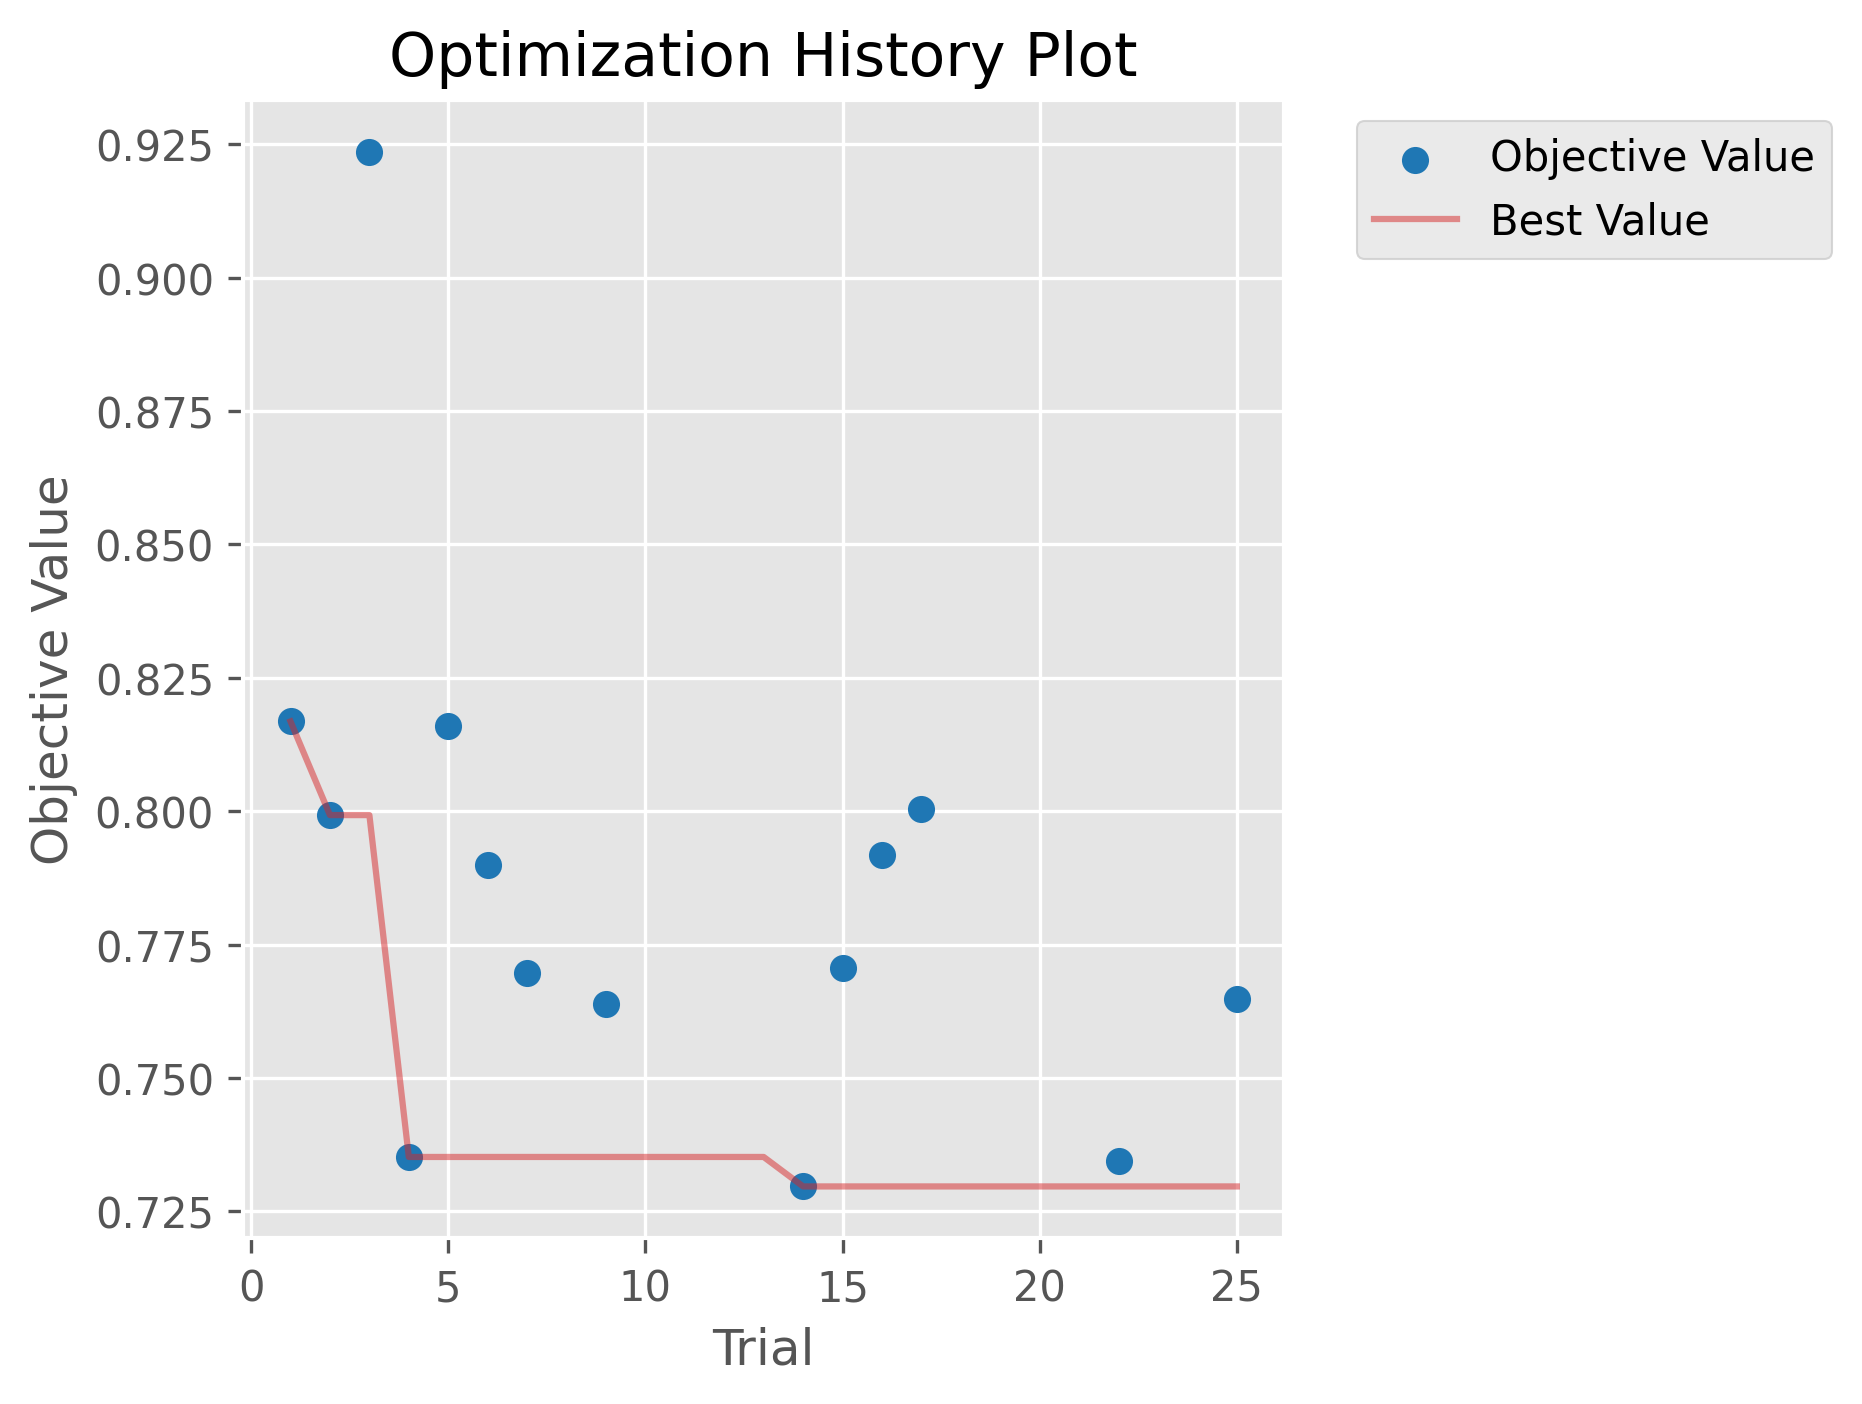
\includegraphics[width=0.8\linewidth]{problem_1_experiments/optuna_studies/pinn_v4_baseline/figures/optimization_history.png}
    \caption{Baseline Optuna optimization history. The objective improves as the study progresses, but the gains eventually plateau, suggesting that the baseline physics-only formulation is fundamentally limited rather than merely under-tuned.}
\end{figure}

\begin{figure}[H]
    \centering
    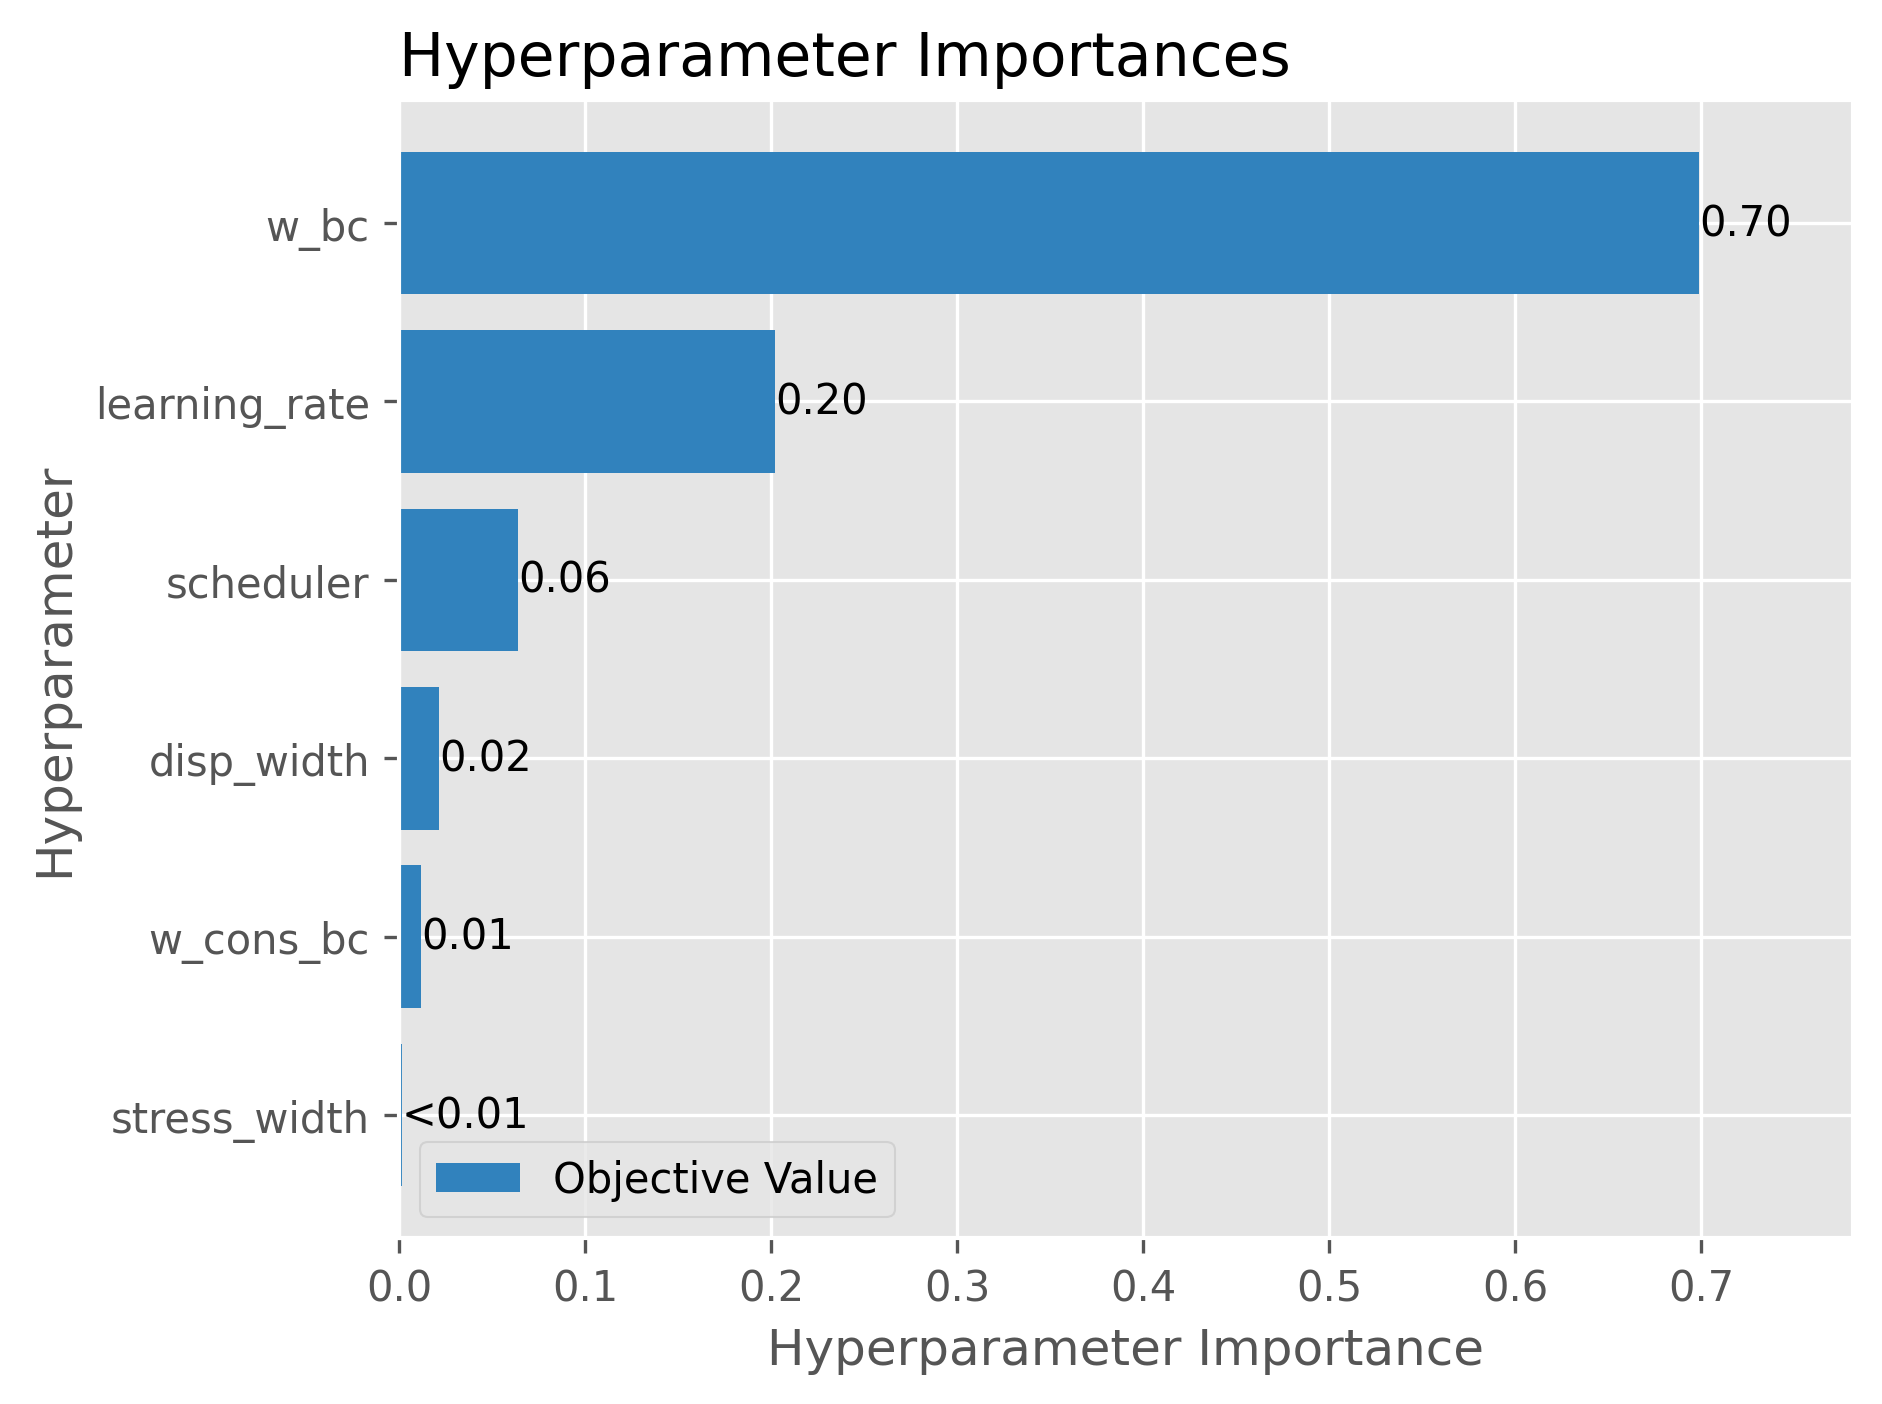
\includegraphics[width=0.8\linewidth]{problem_1_experiments/optuna_studies/pinn_v4_baseline/figures/param_importances.png}
    \caption{Baseline Optuna hyperparameter importance. This plot was used together with the top-trial table to identify which settings mattered most. In practice, it supported the conclusion that network width and loss weighting were more important than the presence of a scheduler.}
\end{figure}

\begin{figure}[H]
    \centering
    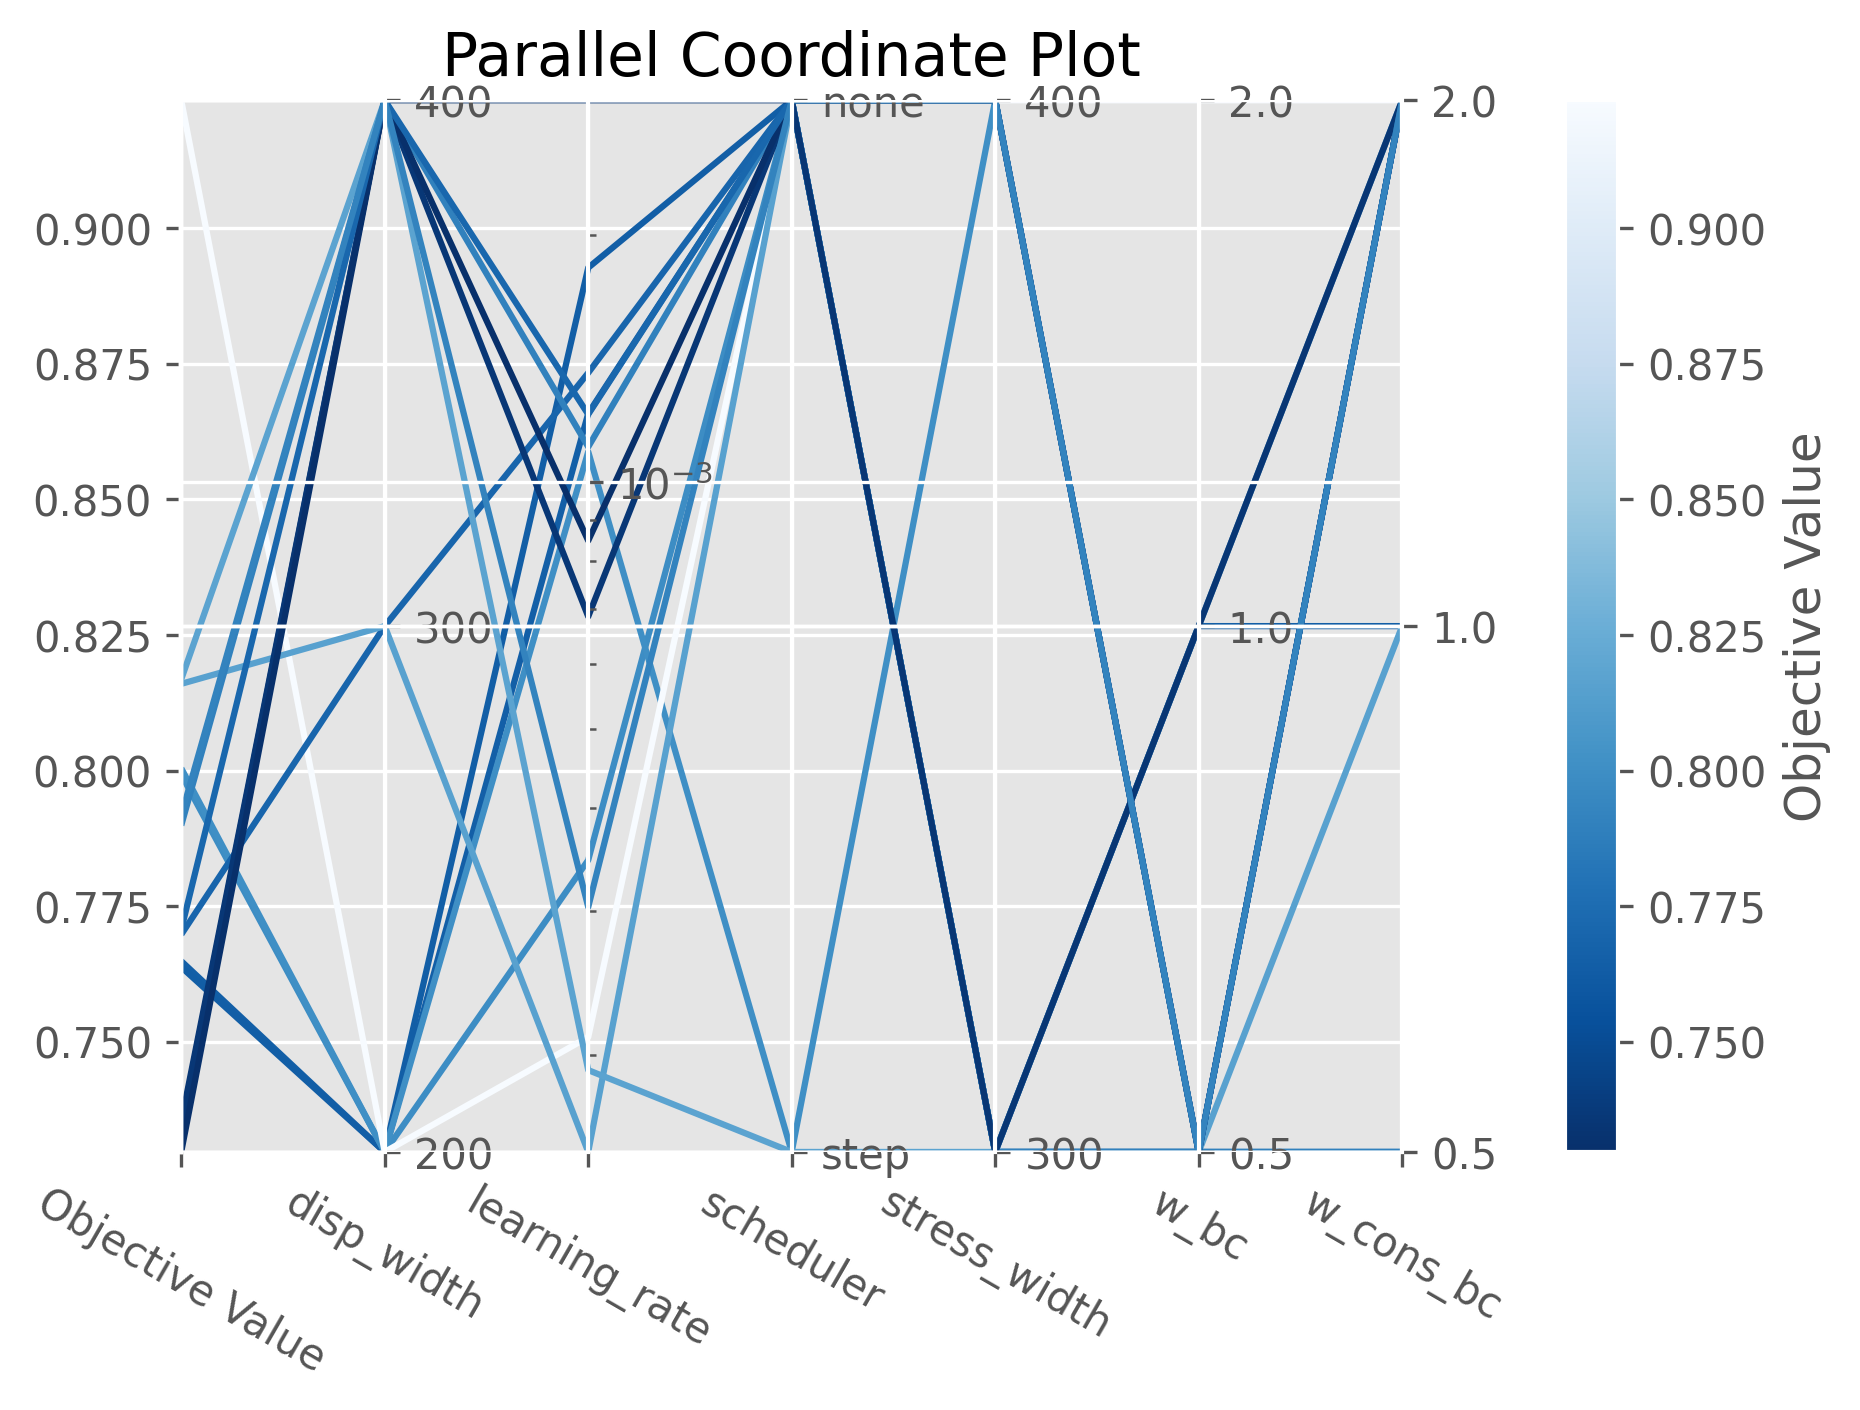
\includegraphics[width=0.8\linewidth]{problem_1_experiments/optuna_studies/pinn_v4_baseline/figures/parallel_coordinate.png}
    \caption{Baseline parallel-coordinate plot. The best baseline trials consistently preferred no scheduler, a wide displacement network, and strong boundary constitutive weighting.}
\end{figure}

\begin{figure}[H]
    \centering
    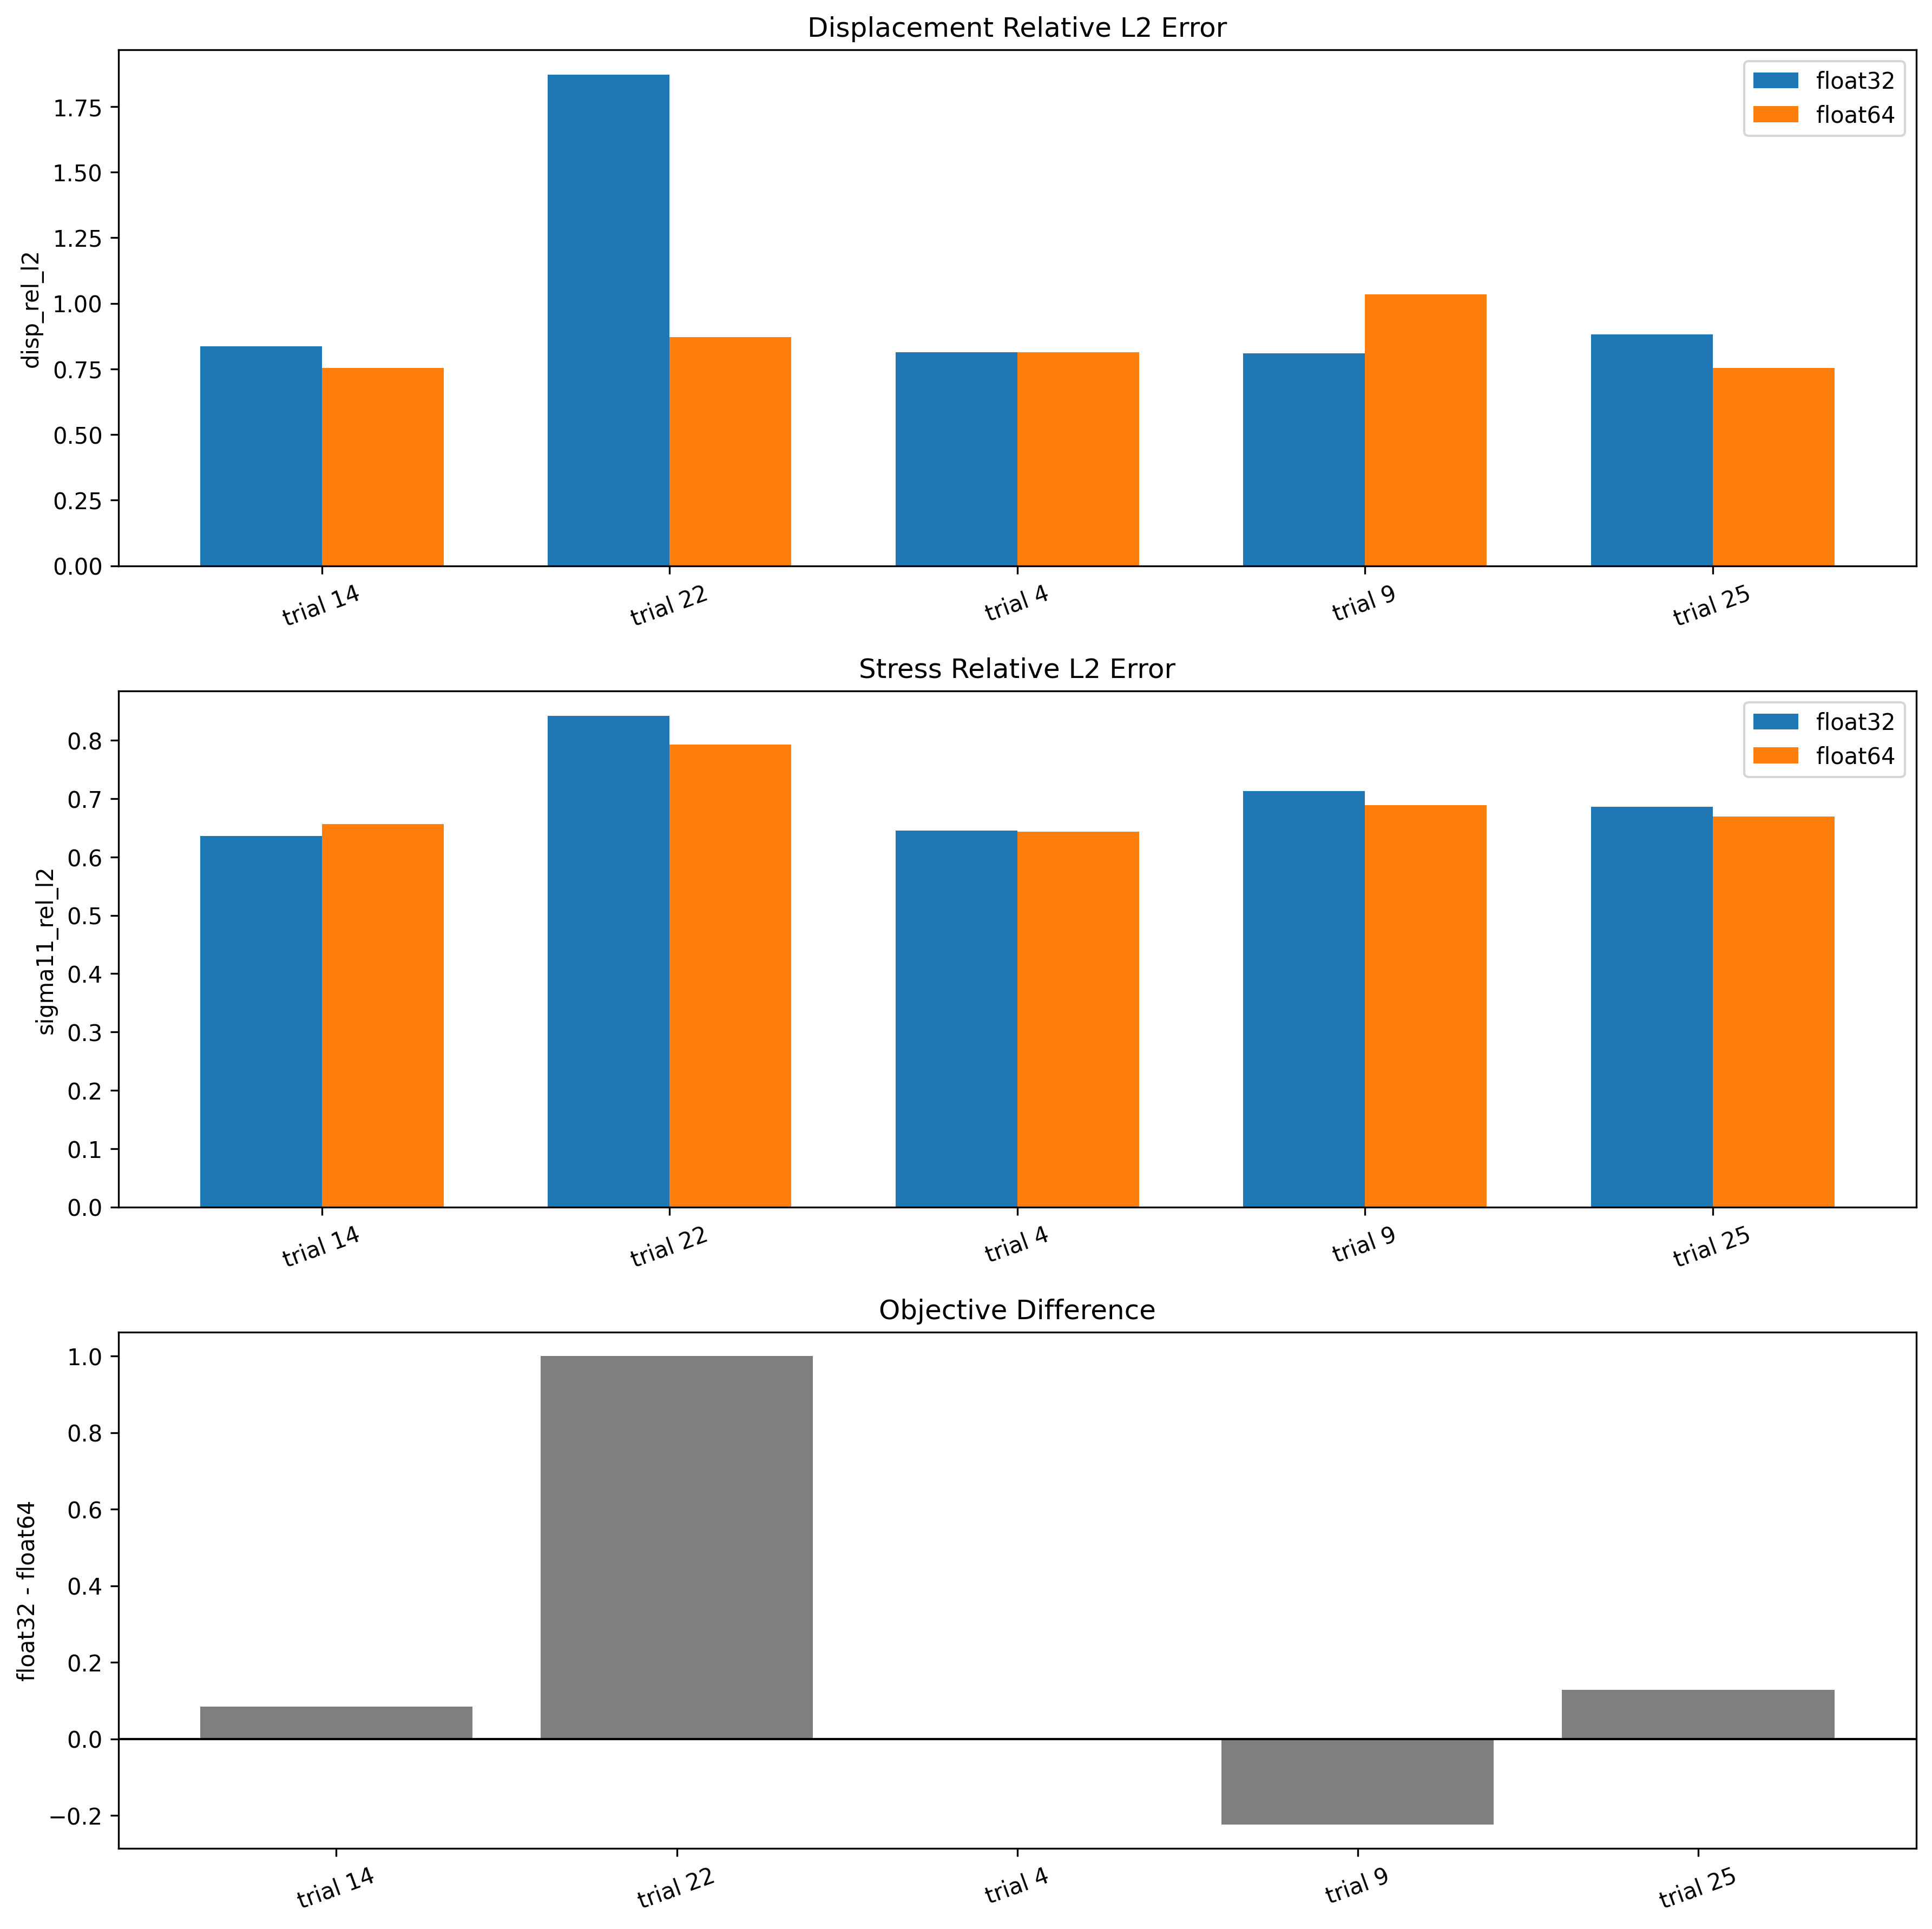
\includegraphics[width=0.8\linewidth]{problem_1_experiments/optuna_studies/pinn_v4_baseline/figures/rerun_float32_vs_float64.png}
    \caption{Baseline float32/MPS vs.\ float64/CPU rerun comparison. This plot shows why float32/MPS was useful for screening but not sufficiently reliable for final model selection.}
\end{figure}

The best baseline Optuna trial used
\[
\texttt{learning\_rate}=8.48\times10^{-4}, \quad
\texttt{disp\_width}=400, \quad
\texttt{stress\_width}=400, \quad
\texttt{scheduler}=\texttt{none},
\]
with \(w_{\mathrm{bc}}=0.5\) and \(w_{\mathrm{cons,bc}}=2.0\). Notably, the top five completed baseline trials all used no scheduler, suggesting that loss balancing was more important than StepLR under the short proxy budget.

For part (e), the best raw Optuna trial used
\[
\texttt{learning\_rate}=2.25\times10^{-4}, \quad
\texttt{disp\_width}=200, \quad
\texttt{stress\_width}=400, \quad
\texttt{scheduler}=\texttt{none},
\]
with \(w_{\mathrm{bc}}=5.0\), \(w_{\mathrm{cons,bc}}=2.0\), and \(w_{\mathrm{data}}=884.24\). This is physically plausible: once supervised displacement data were included, strong boundary weighting and a large data-loss weight became helpful because the model had to satisfy both the PDE and measured displacements.

\begin{figure}[H]
    \centering
    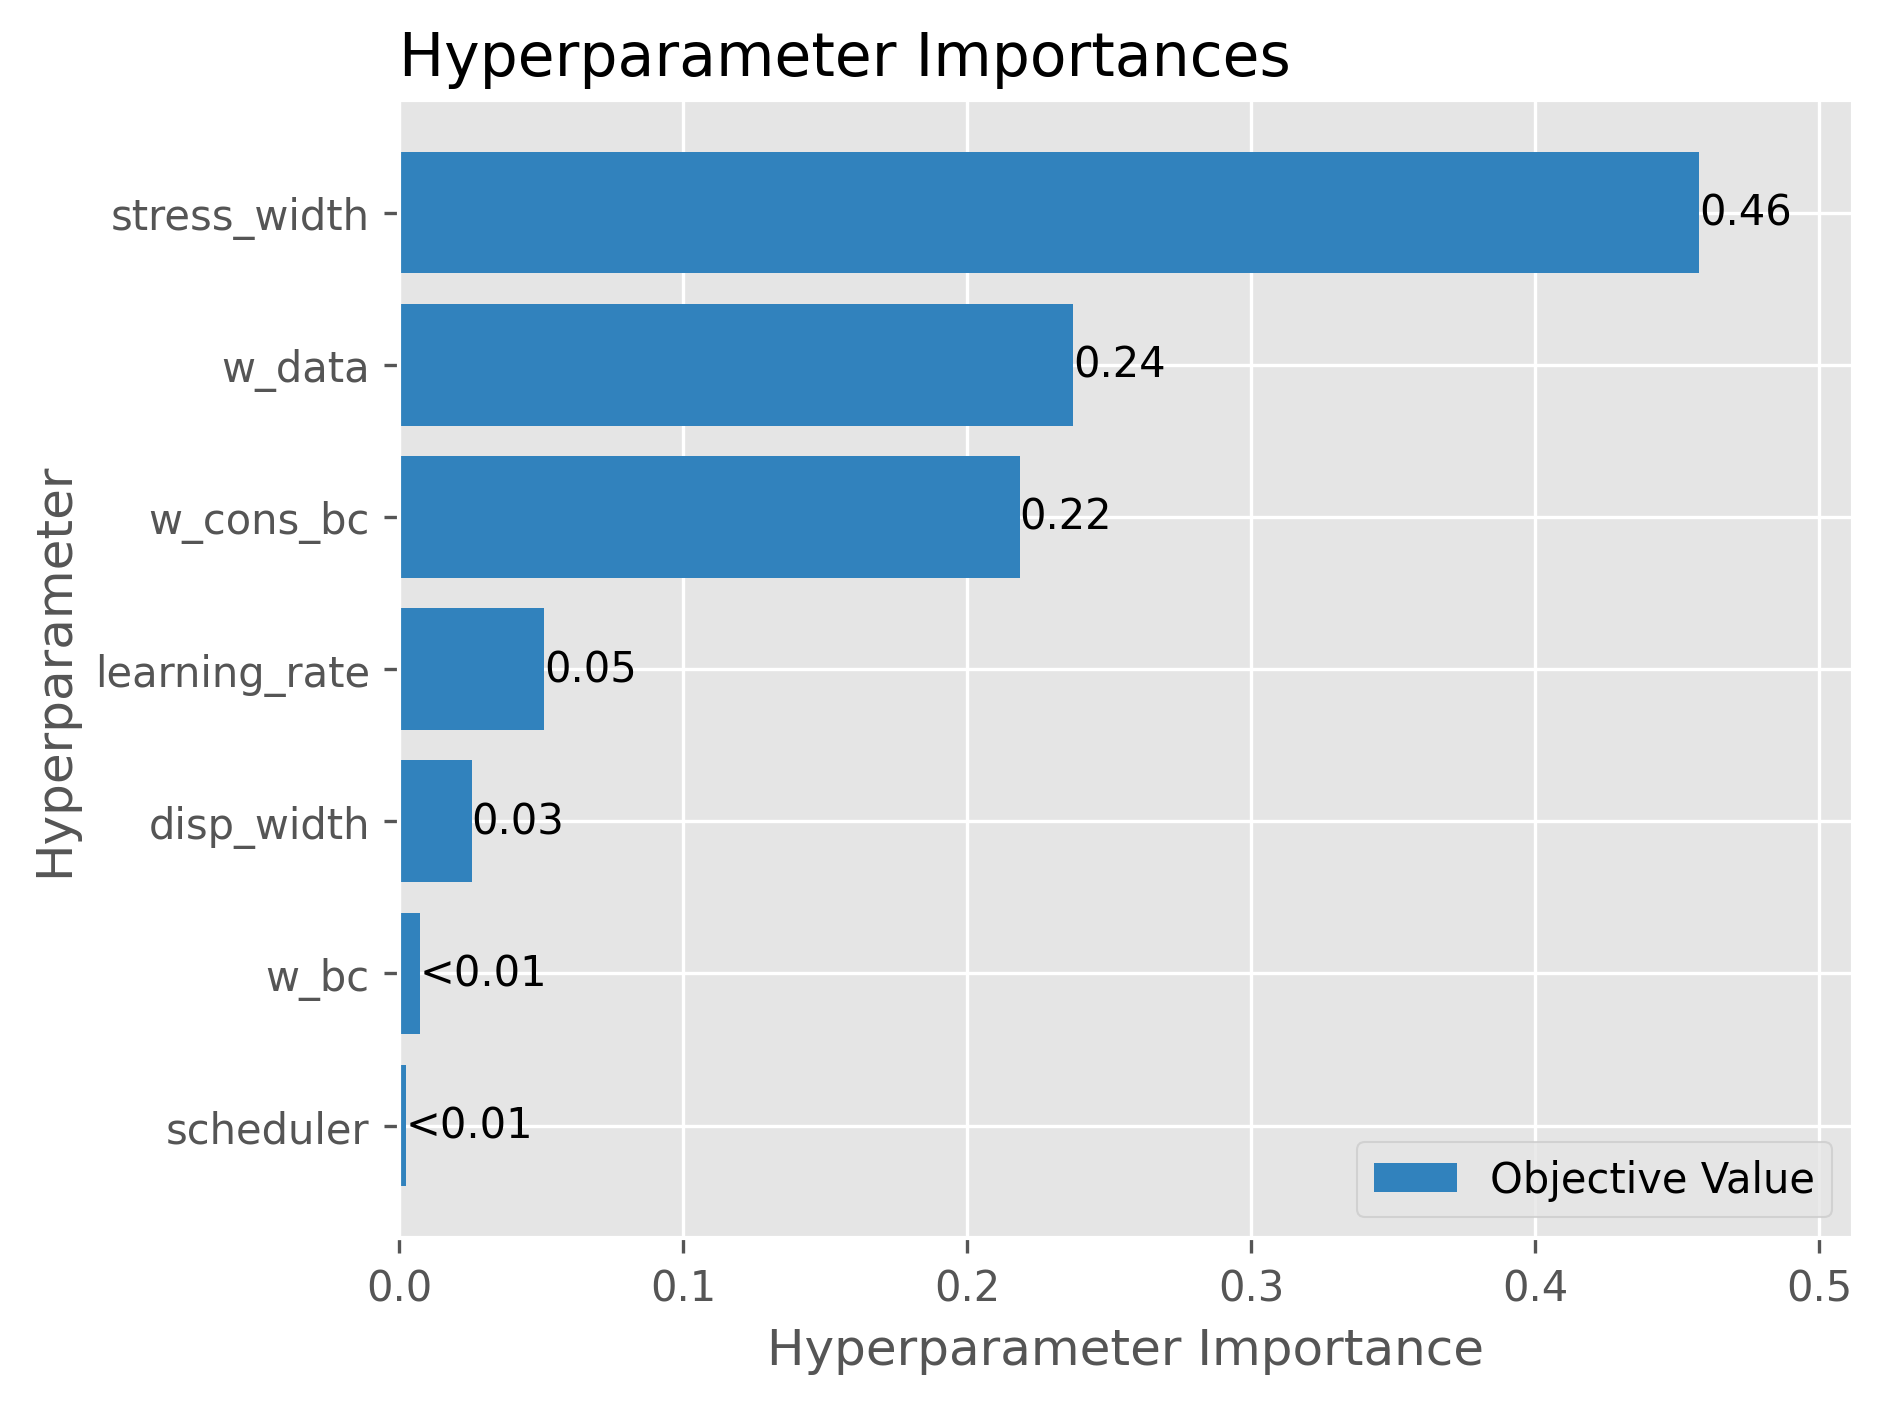
\includegraphics[width=0.8\linewidth]{problem_1_experiments/optuna_studies/pinn_v4_part_e/figures/param_importances.png}
    \caption{Part (e) Optuna hyperparameter importance. The dominant settings shifted once measurement data were included, especially the data-loss and boundary-related weights.}
\end{figure}

\begin{figure}[H]
    \centering
    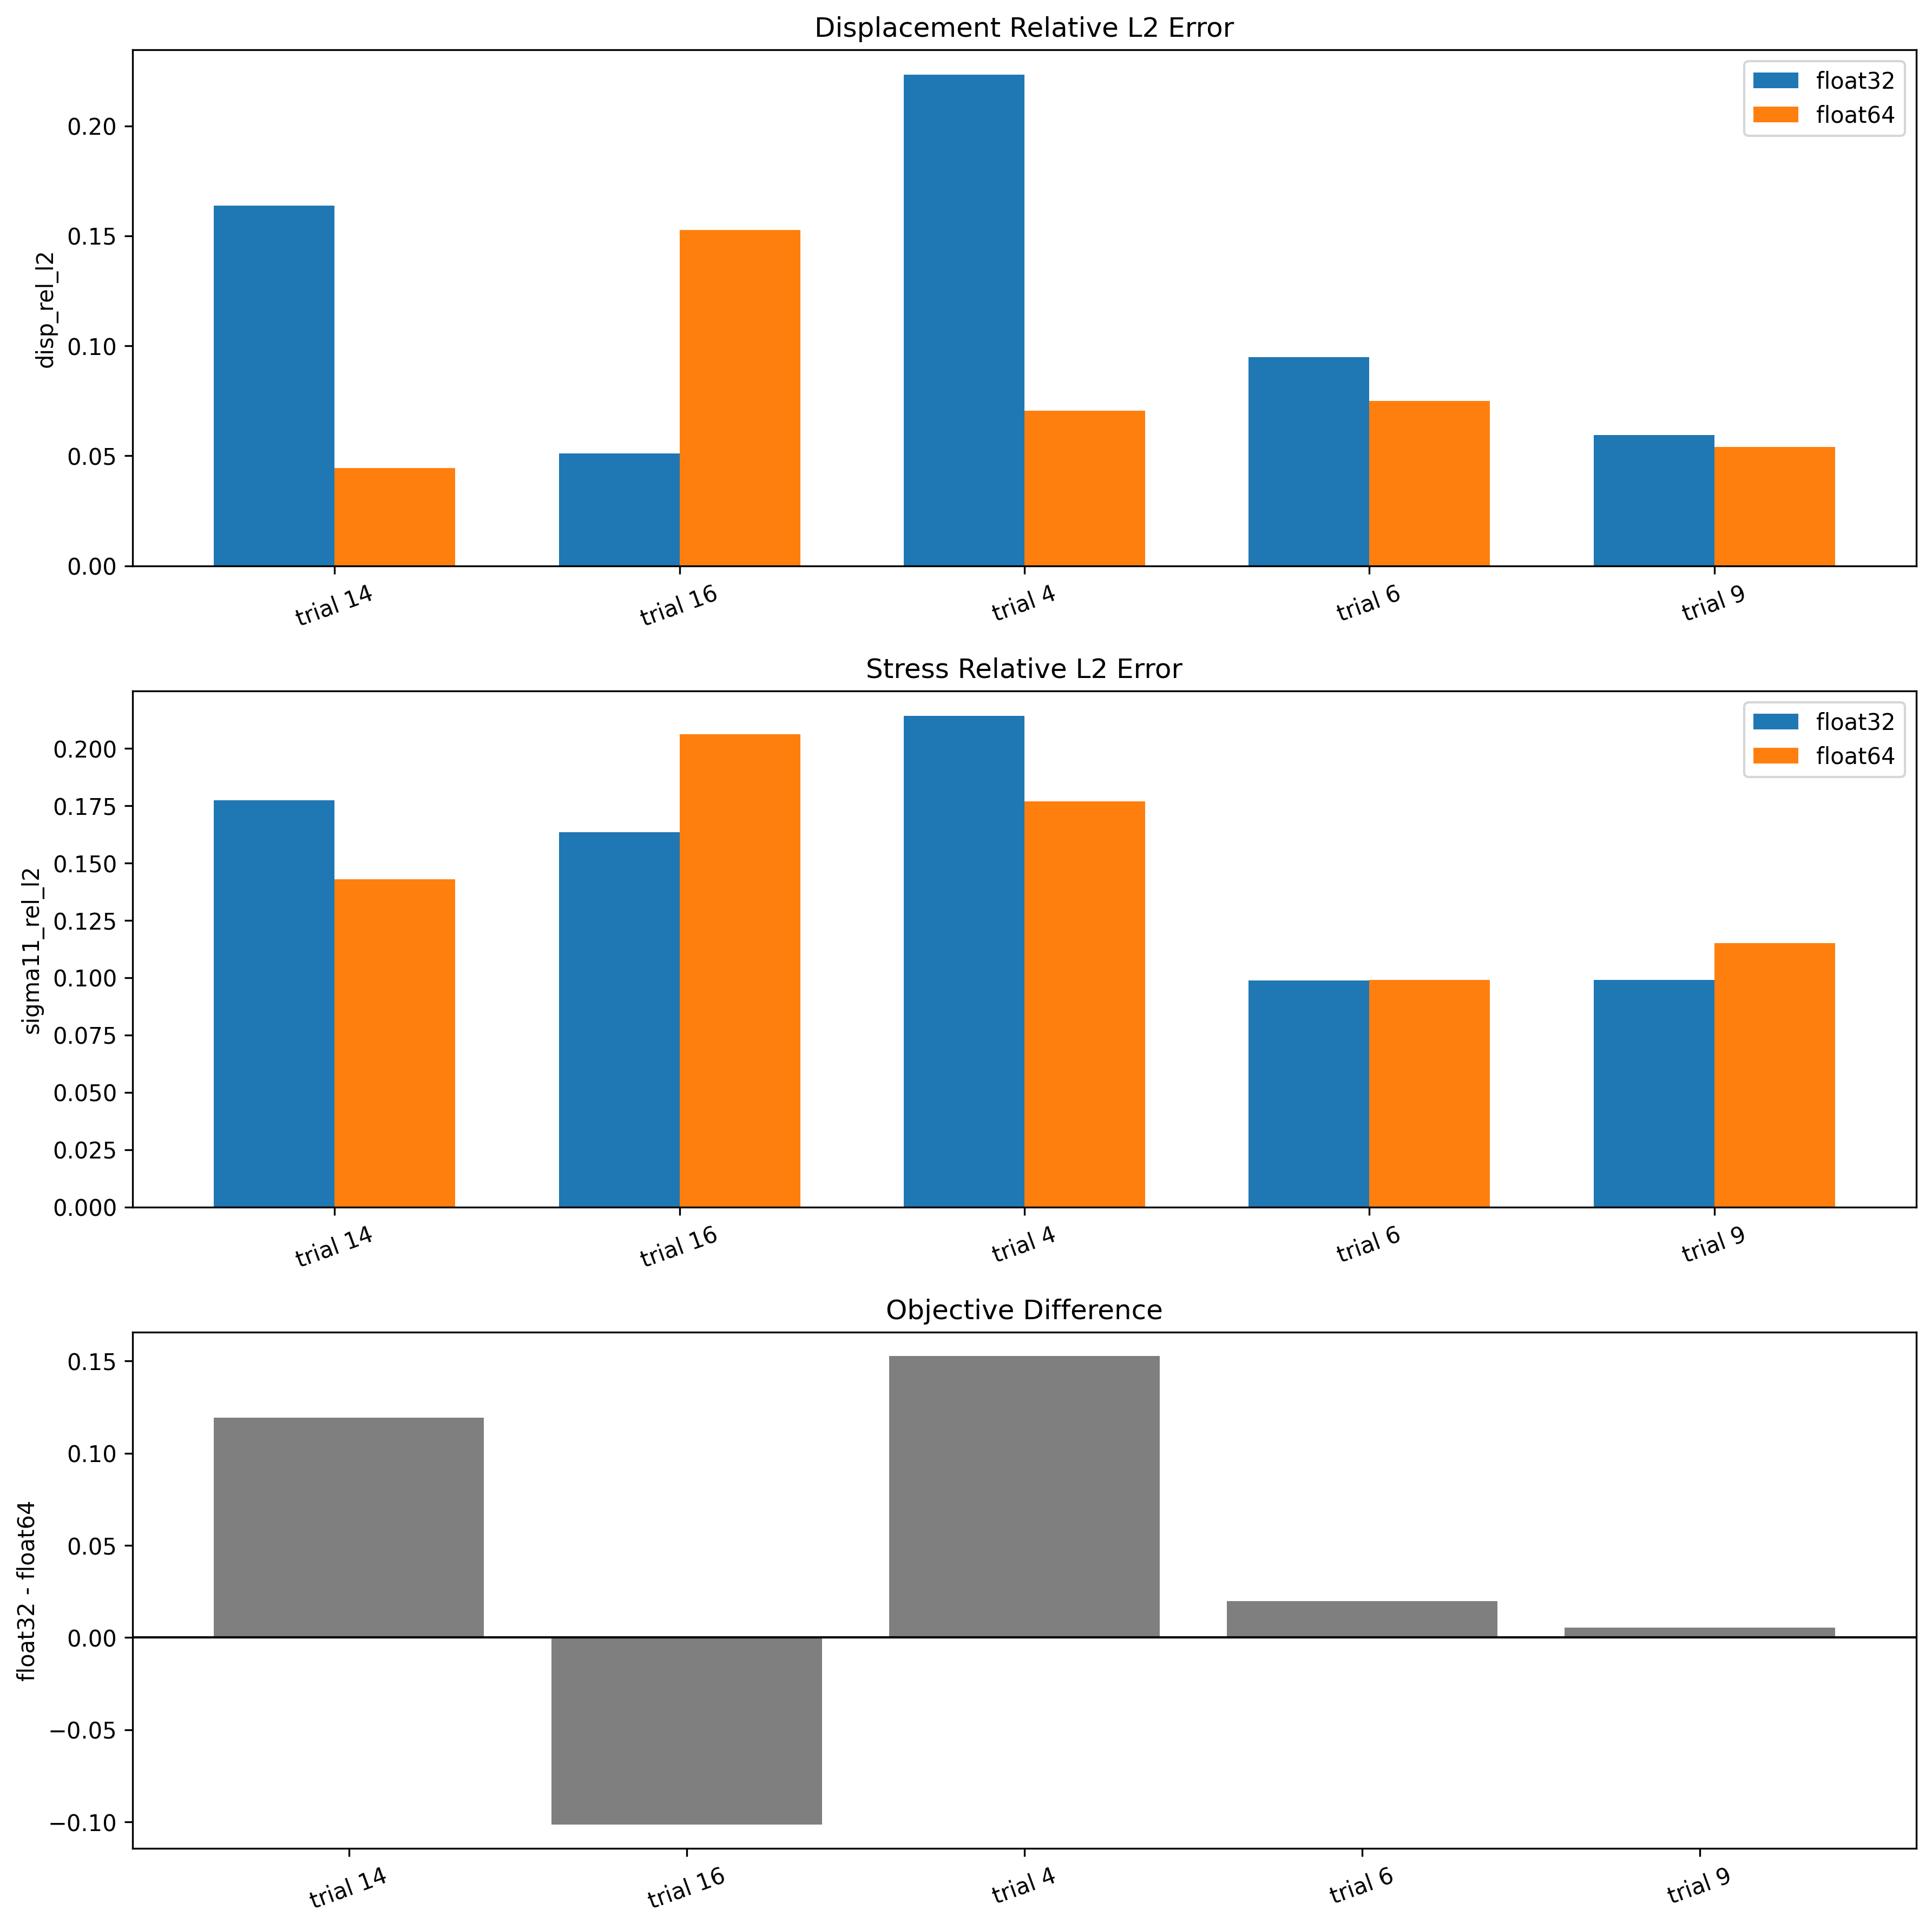
\includegraphics[width=0.8\linewidth]{problem_1_experiments/optuna_studies/pinn_v4_part_e/figures/rerun_float32_vs_float64.png}
    \caption{Part (e) float32/MPS vs.\ float64/CPU rerun comparison. Although the average float32--float64 gap was smaller than in the baseline study, it was still large enough to justify final model selection in float64.}
\end{figure}

The tuning process therefore led to two clear conclusions. First, the baseline physics-only PINN remained hard to make accurate even after systematic tuning. Second, the data-assisted PINN responded strongly to the inclusion of measured data and to careful tuning of the relative loss weights.

\subsection*{Physics-Only PINN Results}

The canonical physics-only run was \path{problem1_20260315_165315_full_nodata_seed1234}. It was trained for 100,000 epochs on CPU and achieved its best tracked loss of \(2.75\times10^{-6}\) at epoch 75,096. Judged by training loss alone, this appears to be a successful optimization. However, the FEM comparison shows that this is misleading.

\begin{table}[H]
\centering
\begin{tabular}{lr}
\toprule
Metric & Physics-only PINN \\
\midrule
Best training loss & \(2.75\times10^{-6}\) \\
Displacement RMSE & 0.01709 \\
Displacement relative \(L_2\) & 0.84411 \\
\(u\) relative \(L_2\) & 0.74376 \\
\(v\) relative \(L_2\) & 1.40221 \\
\(\sigma_{11}\) relative \(L_2\) & 0.67764 \\
\(\sigma_{22}\) relative \(L_2\) & 1.64342 \\
\(\sigma_{12}\) relative \(L_2\) & 1.06227 \\
\bottomrule
\end{tabular}
\caption{Final quantitative results for the physics-only PINN.}
\end{table}

These values are too large to claim that the FEM solution has been recovered well. The displacement error is large, and the \(\sigma_{22}\) and \(\sigma_{12}\) stress components are especially poor.

\begin{figure}[H]
    \centering
    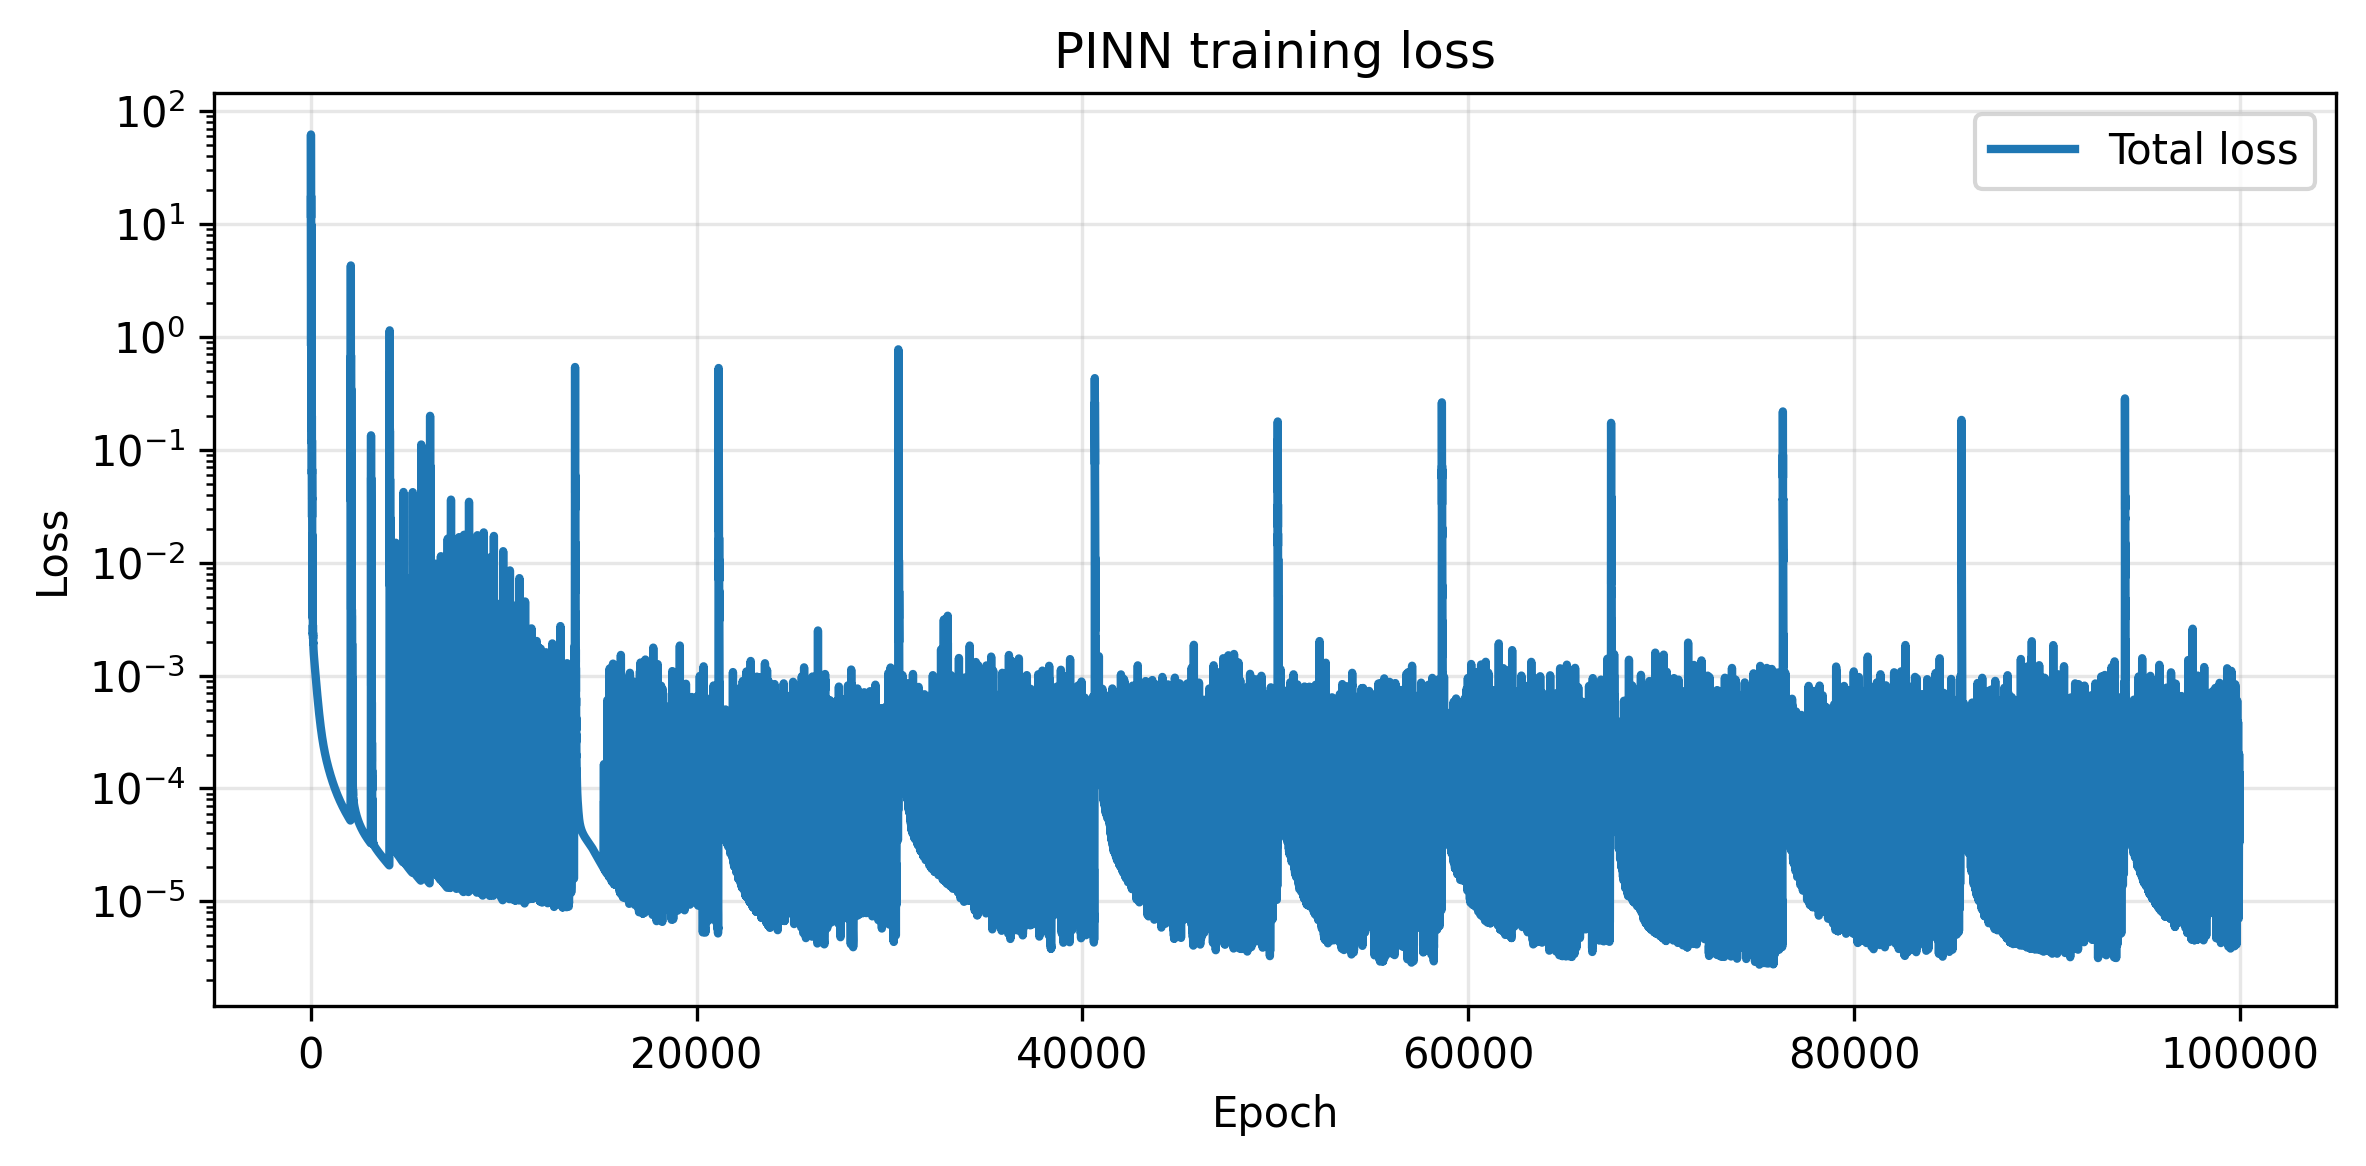
\includegraphics[width=0.78\linewidth]{problem_1_figures/problem1_20260315_165315_full_nodata_seed1234/training_loss.png}
    \caption{Physics-only PINN training loss. The loss decreases strongly, but this alone does not imply external accuracy.}
\end{figure}

\begin{figure}[H]
    \centering
    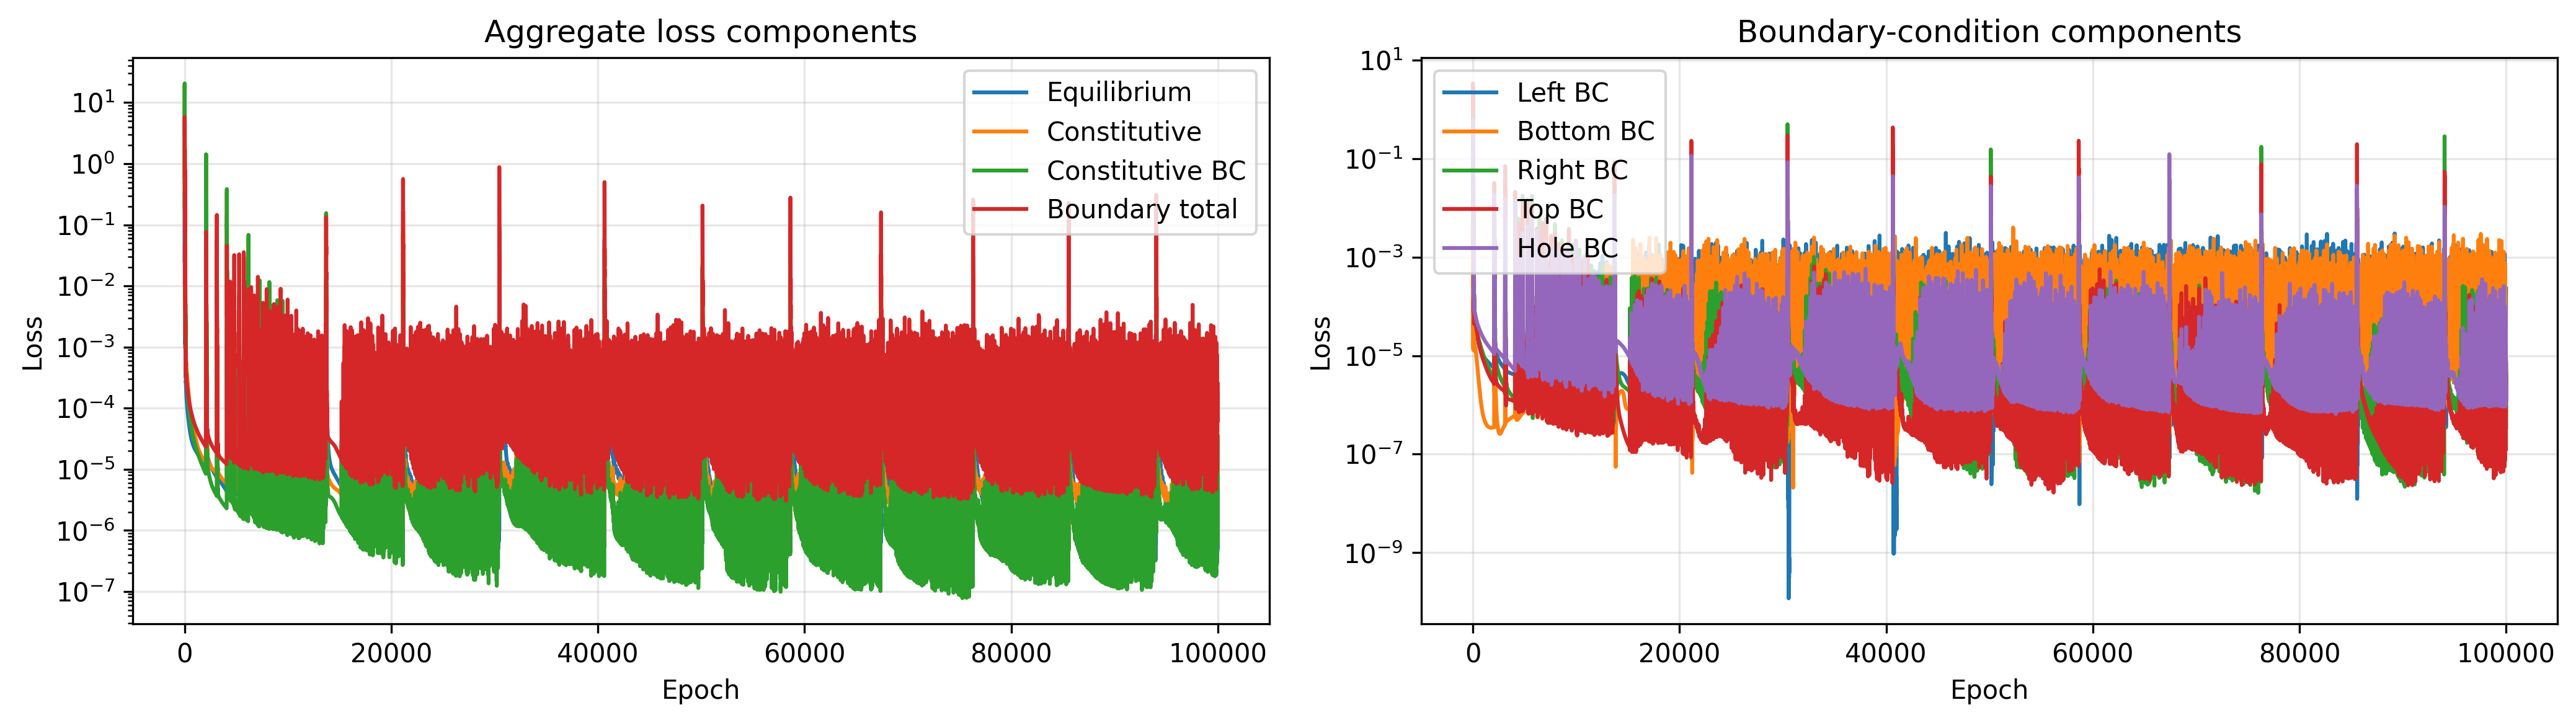
\includegraphics[width=0.78\linewidth]{problem_1_figures/problem1_20260315_165315_full_nodata_seed1234/loss_components.png}
    \caption{Physics-only PINN loss components. The model is clearly learning to satisfy the internal equilibrium, constitutive, and boundary objectives.}
\end{figure}

\begin{figure}[H]
    \centering
    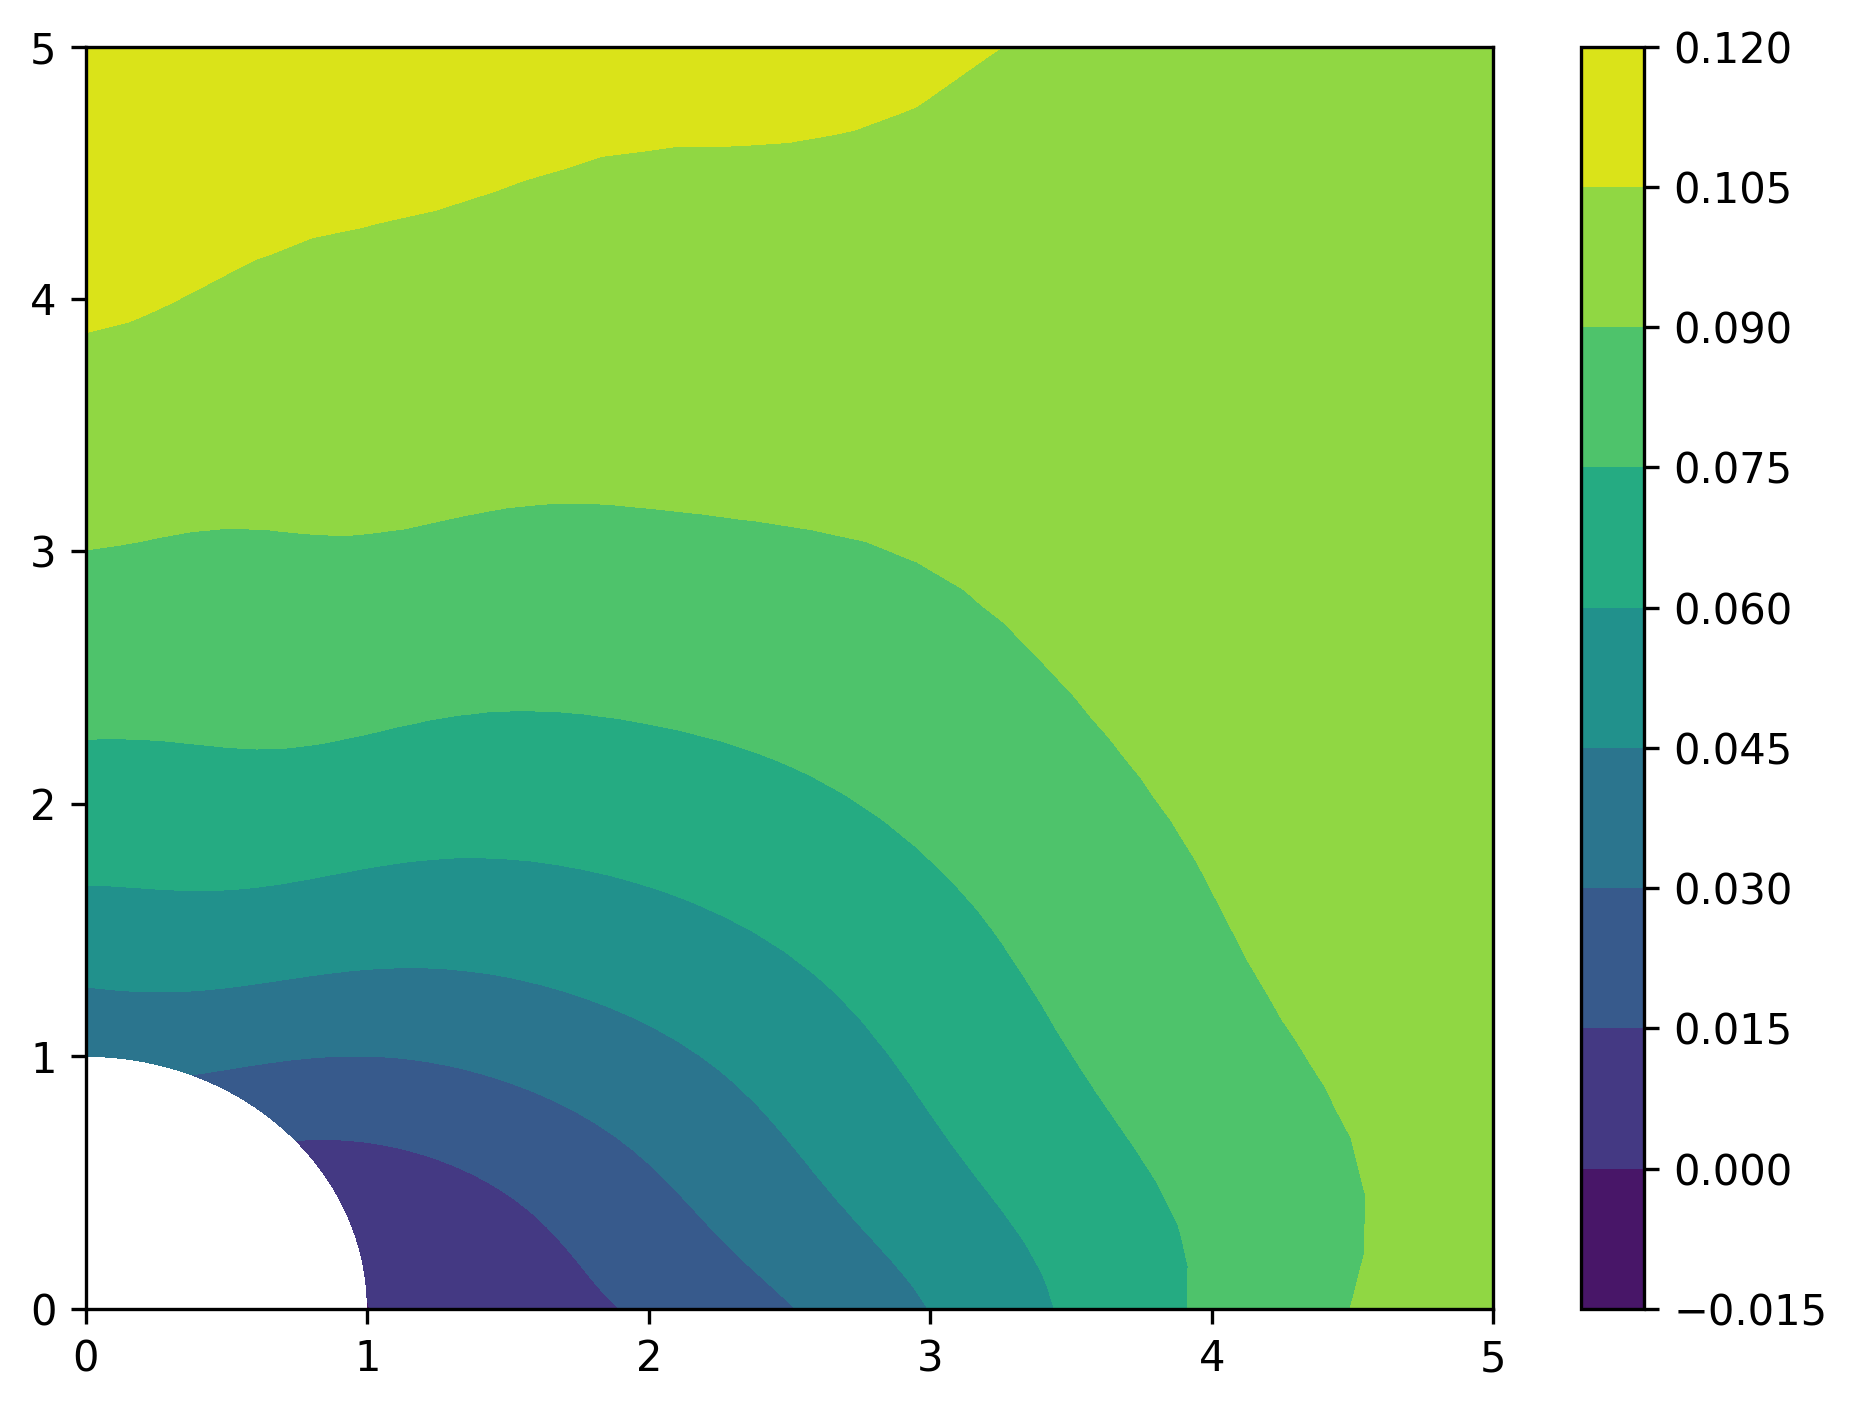
\includegraphics[width=0.72\linewidth]{problem_1_figures/problem1_20260315_165315_full_nodata_seed1234/stress_sigma11.png}
    \caption{Physics-only tensile stress field \(\sigma_{11}\). The field looks plausible in the sense that a stress concentration forms around the hole, but the FEM comparison shows that the detailed stress distribution is still inaccurate.}
\end{figure}

\begin{figure}[H]
    \centering
    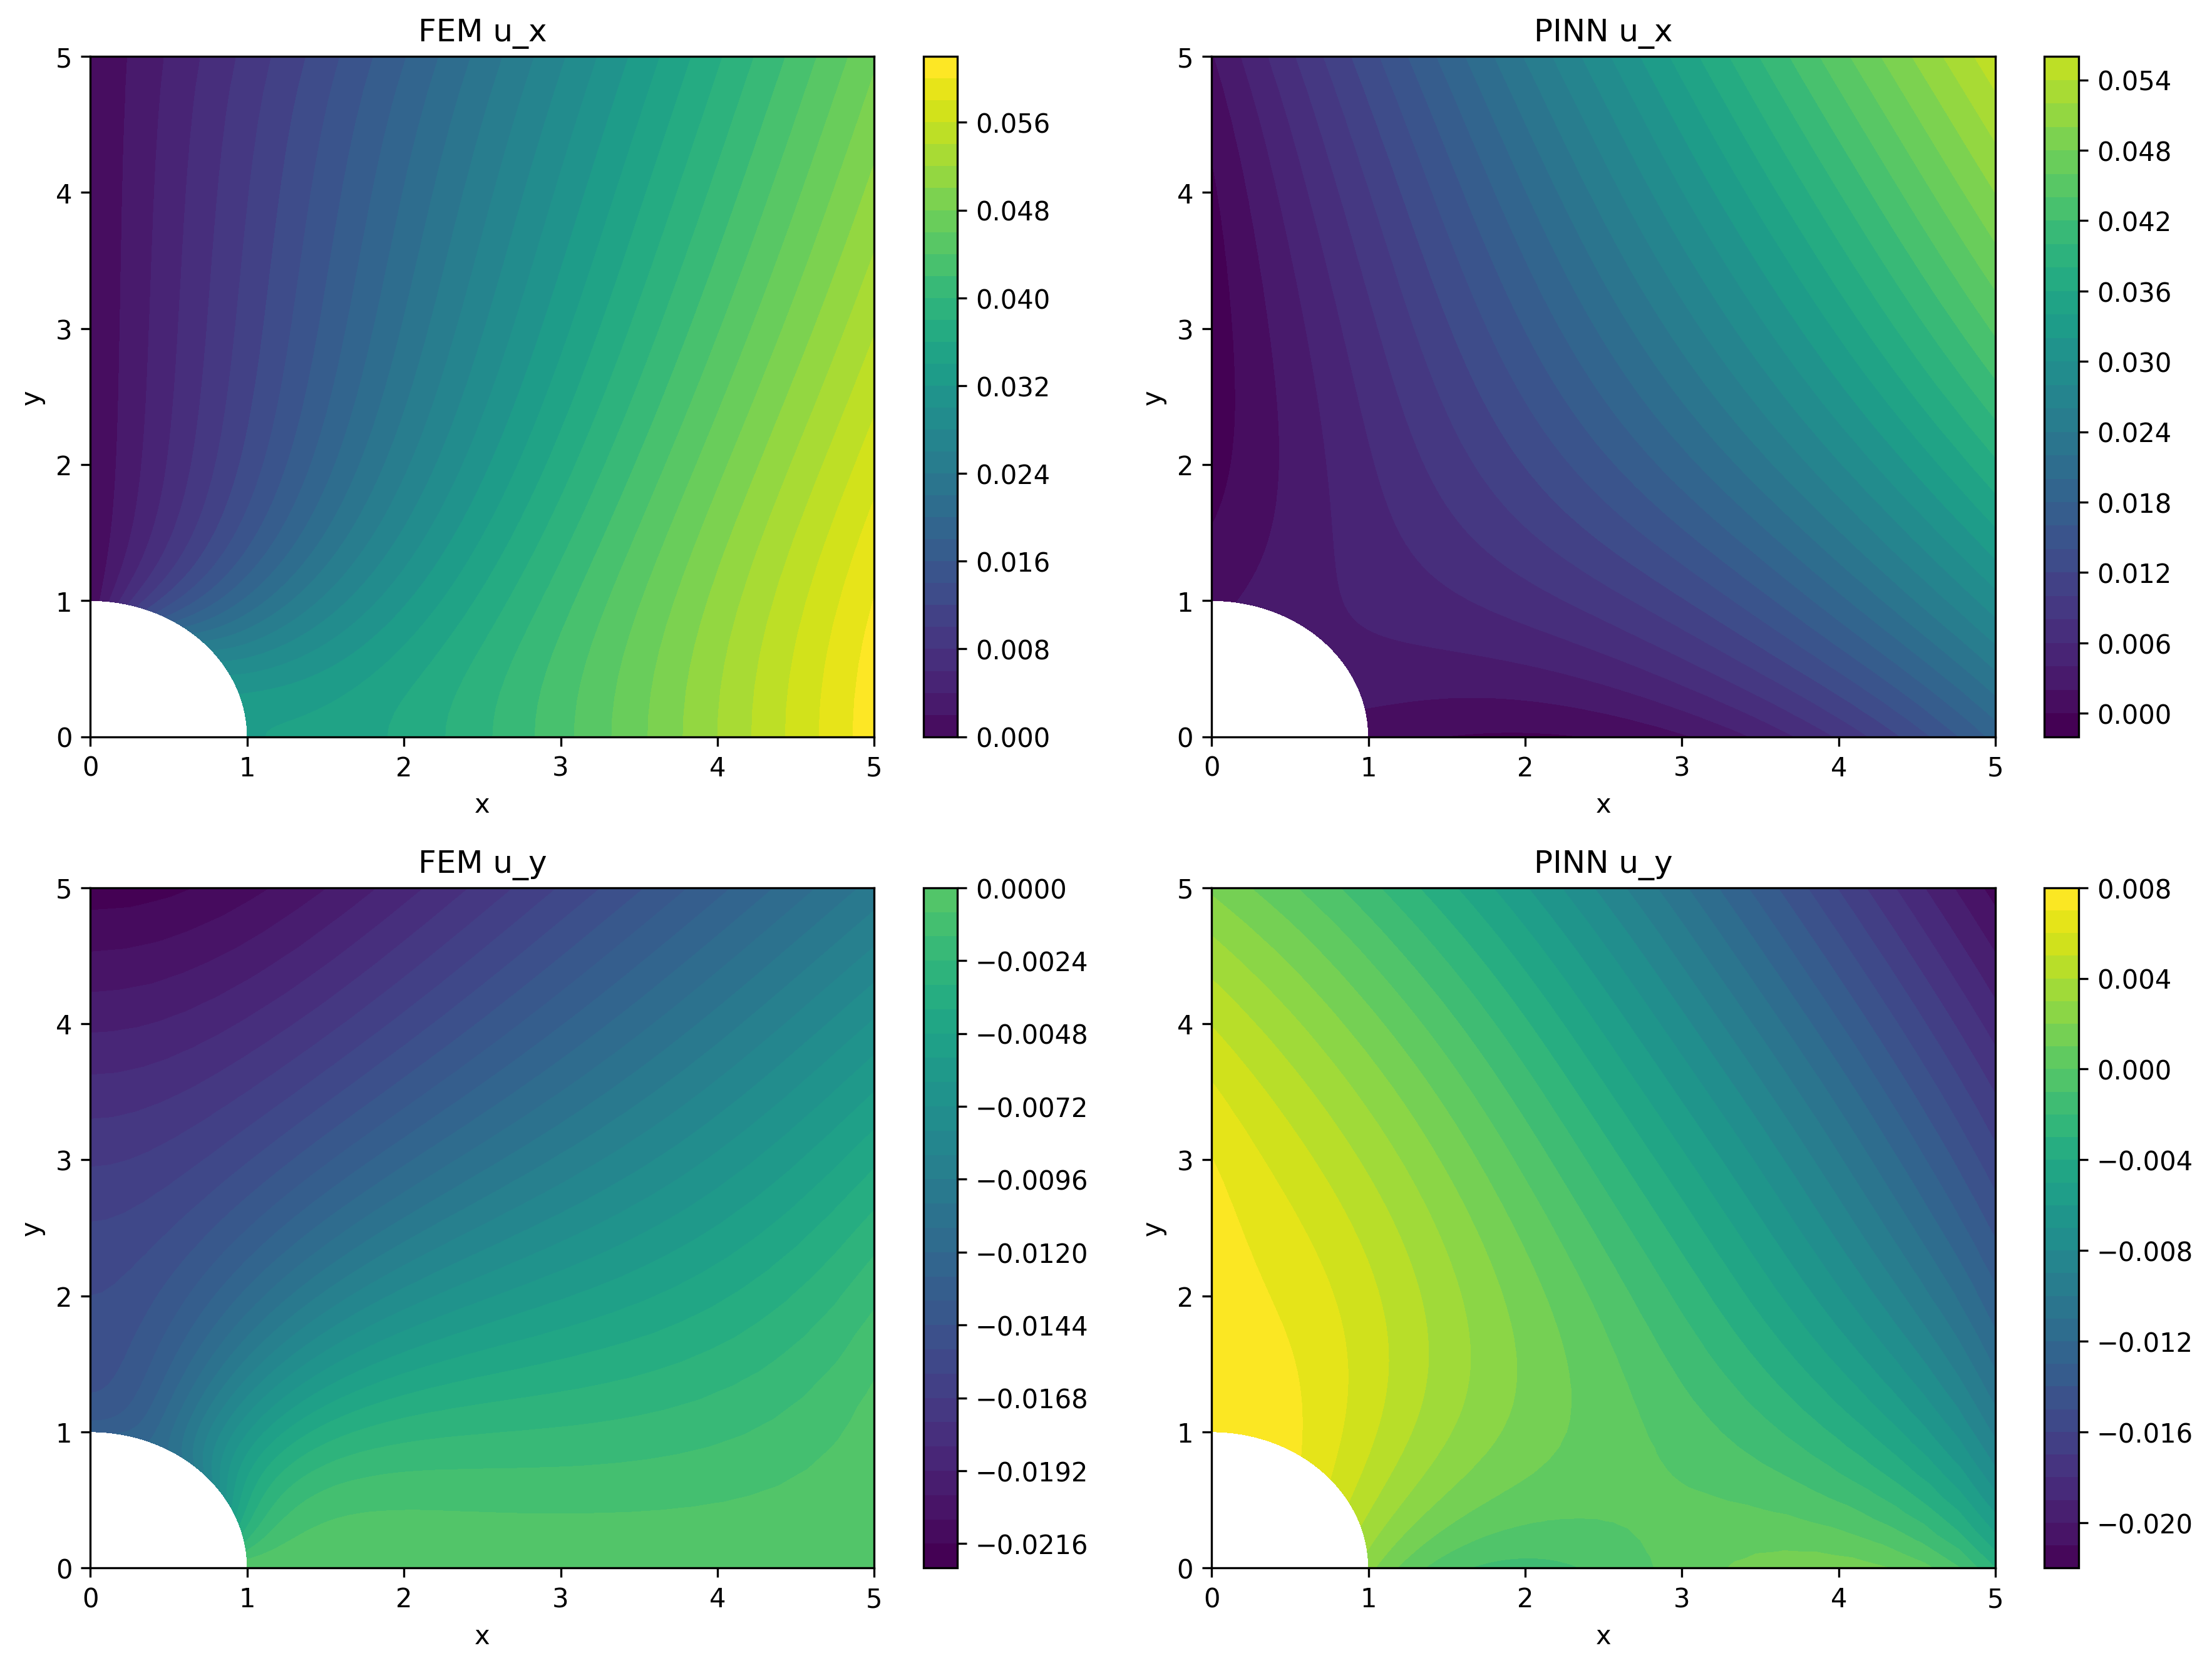
\includegraphics[width=\linewidth]{problem_1_figures/problem1_20260315_165315_full_nodata_seed1234/fem_vs_pinn_displacement.png}
    \caption{Physics-only FEM-vs-PINN displacement comparison. The broad deformation pattern is captured, but the mismatch remains substantial throughout the domain.}
\end{figure}

\begin{figure}[H]
    \centering
    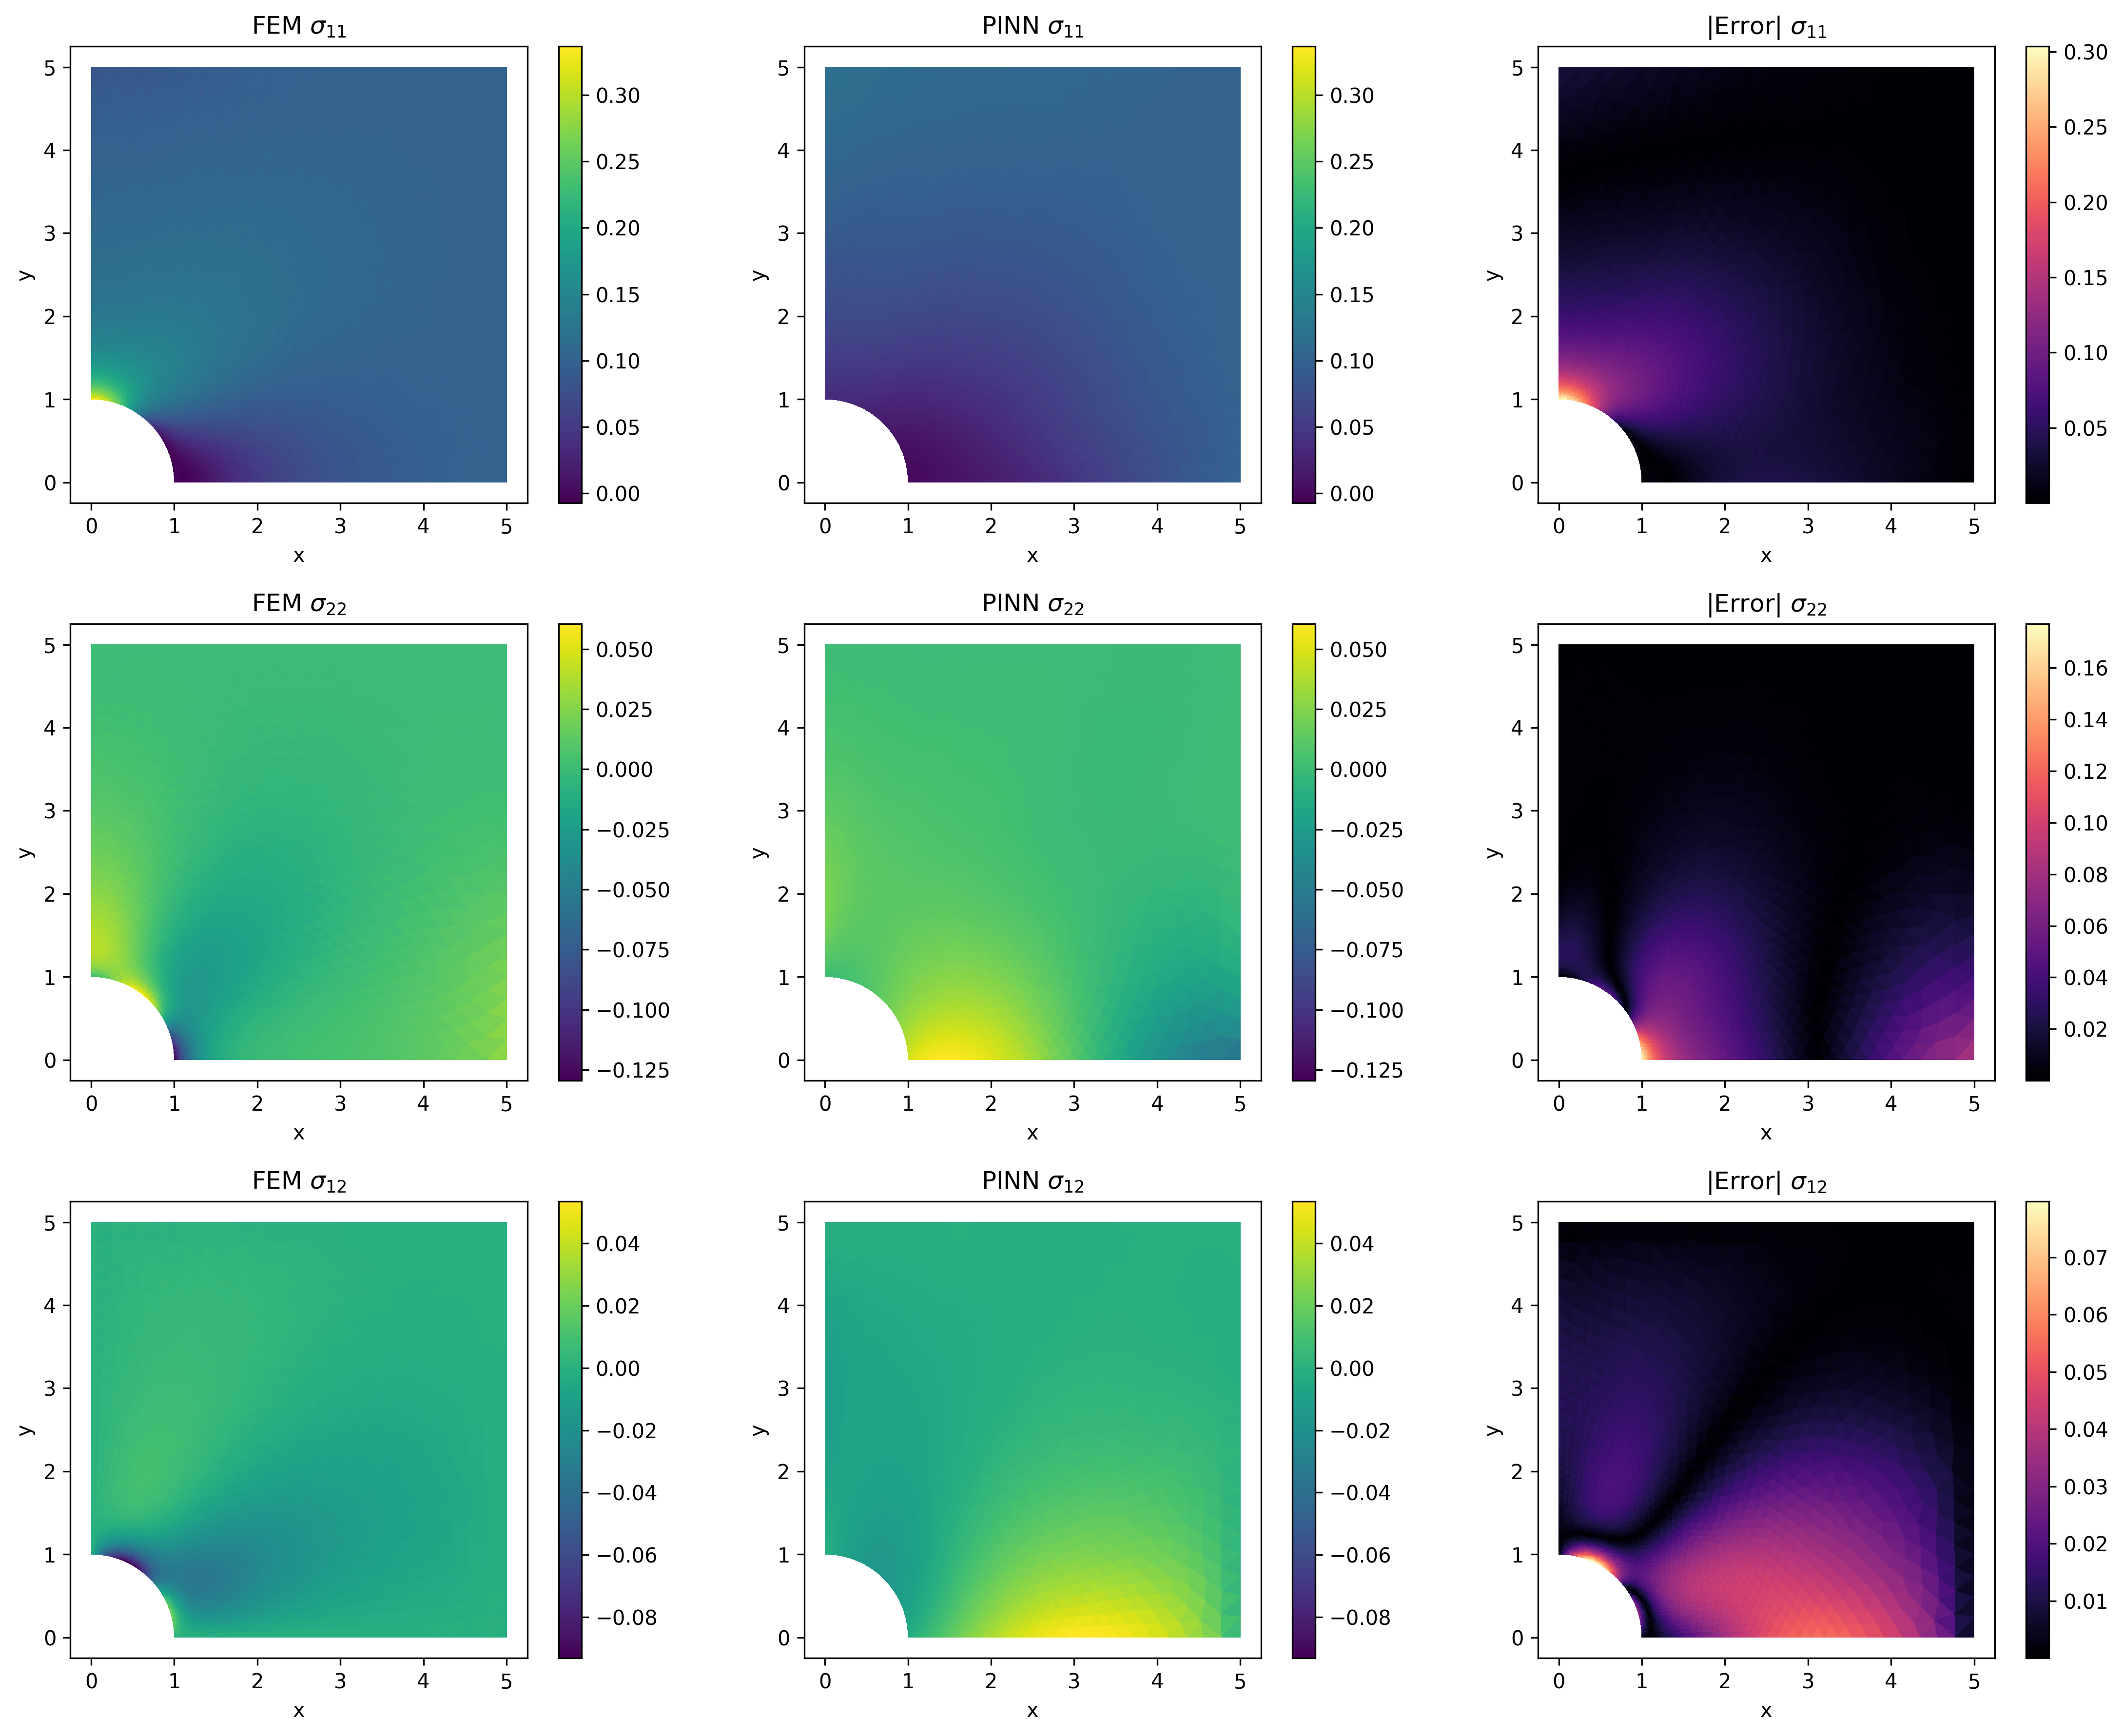
\includegraphics[width=\linewidth]{problem_1_figures/problem1_20260315_165315_full_nodata_seed1234/fem_vs_pinn_stress_components.png}
    \caption{Physics-only FEM-vs-PINN stress comparison. The \(\sigma_{11}\) field is partially captured, but the transverse and shear stress components remain weak.}
\end{figure}

\begin{figure}[H]
    \centering
    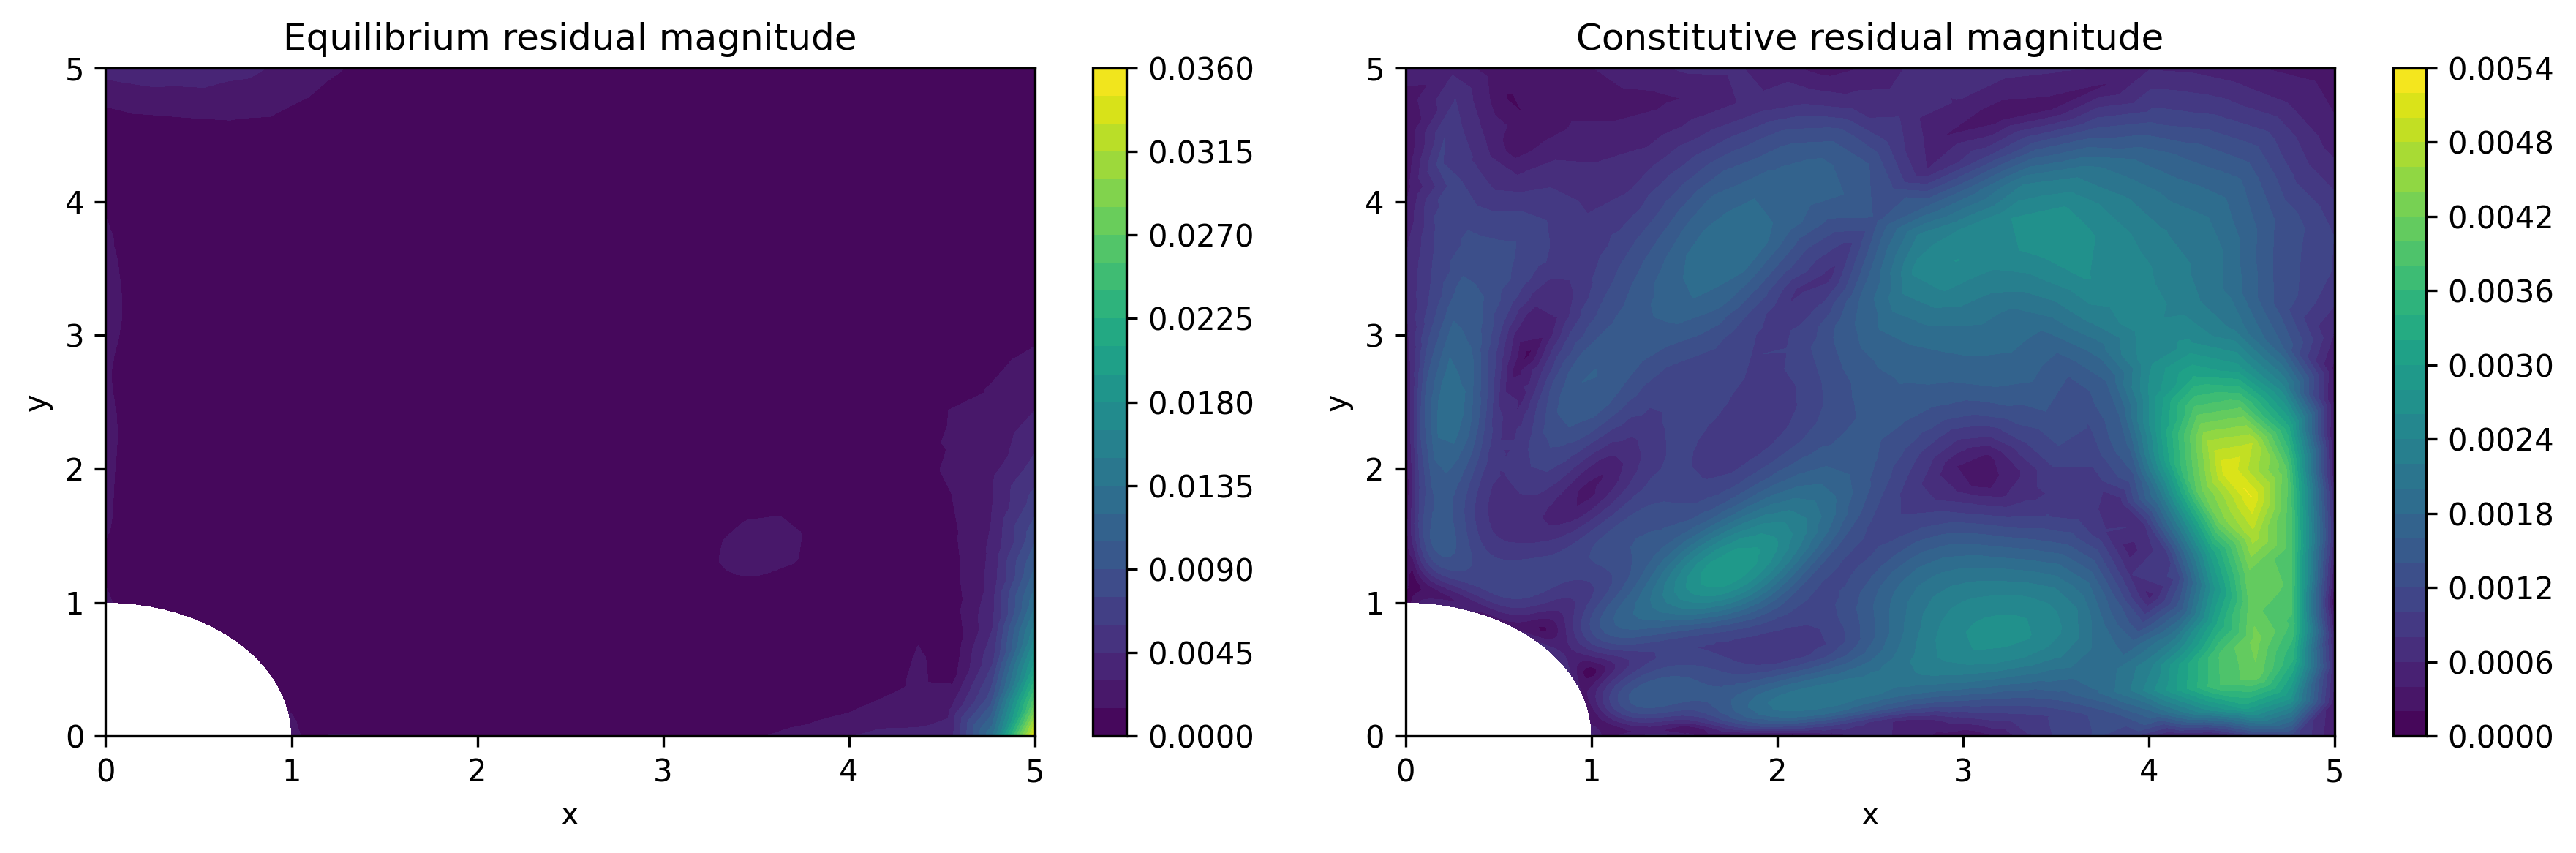
\includegraphics[width=0.9\linewidth]{problem_1_figures/problem1_20260315_165315_full_nodata_seed1234/residual_spatial_maps.png}
    \caption{Physics-only residual spatial maps. The most difficult regions are localized around the hole, where the stress concentration is strongest.}
\end{figure}

The physics-only results therefore reveal the main limitation of the baseline PINN. The model learned to satisfy its own physics-inspired objective extremely well, yet it still failed to reproduce the FEM solution accurately enough for a convincing final answer.

\subsection*{(e) Data-Assisted PINN Results}

The canonical data-assisted run was \path{problem1_20260315_203703_full_data_seed1234}. This model was trained for 50,000 epochs on CPU and included the 50 provided displacement measurements in the loss. Its best tracked loss, \(1.86\times10^{-4}\), was higher than the best loss of the physics-only PINN, but its FEM agreement was dramatically better.

\begin{table}[H]
\centering
\begin{tabular}{lr}
\toprule
Metric & Data-assisted PINN \\
\midrule
Best training loss & \(1.86\times10^{-4}\) \\
Displacement RMSE & 0.000479 \\
Displacement relative \(L_2\) & 0.02368 \\
\(u\) relative \(L_2\) & 0.01766 \\
\(v\) relative \(L_2\) & 0.05019 \\
\(\sigma_{11}\) relative \(L_2\) & 0.07000 \\
\(\sigma_{22}\) relative \(L_2\) & 0.40619 \\
\(\sigma_{12}\) relative \(L_2\) & 0.28971 \\
\bottomrule
\end{tabular}
\caption{Final quantitative results for the data-assisted PINN.}
\end{table}

Relative to the physics-only PINN, the improvement is very large:
\begin{itemize}[itemsep=0.25em]
    \item displacement relative \(L_2\) error reduced by about 97.2\%,
    \item \(\sigma_{11}\) relative \(L_2\) error reduced by about 89.7\%,
    \item \(\sigma_{22}\) relative \(L_2\) error reduced by about 75.3\%,
    \item \(\sigma_{12}\) relative \(L_2\) error reduced by about 72.7\%.
\end{itemize}

\begin{figure}[H]
    \centering
    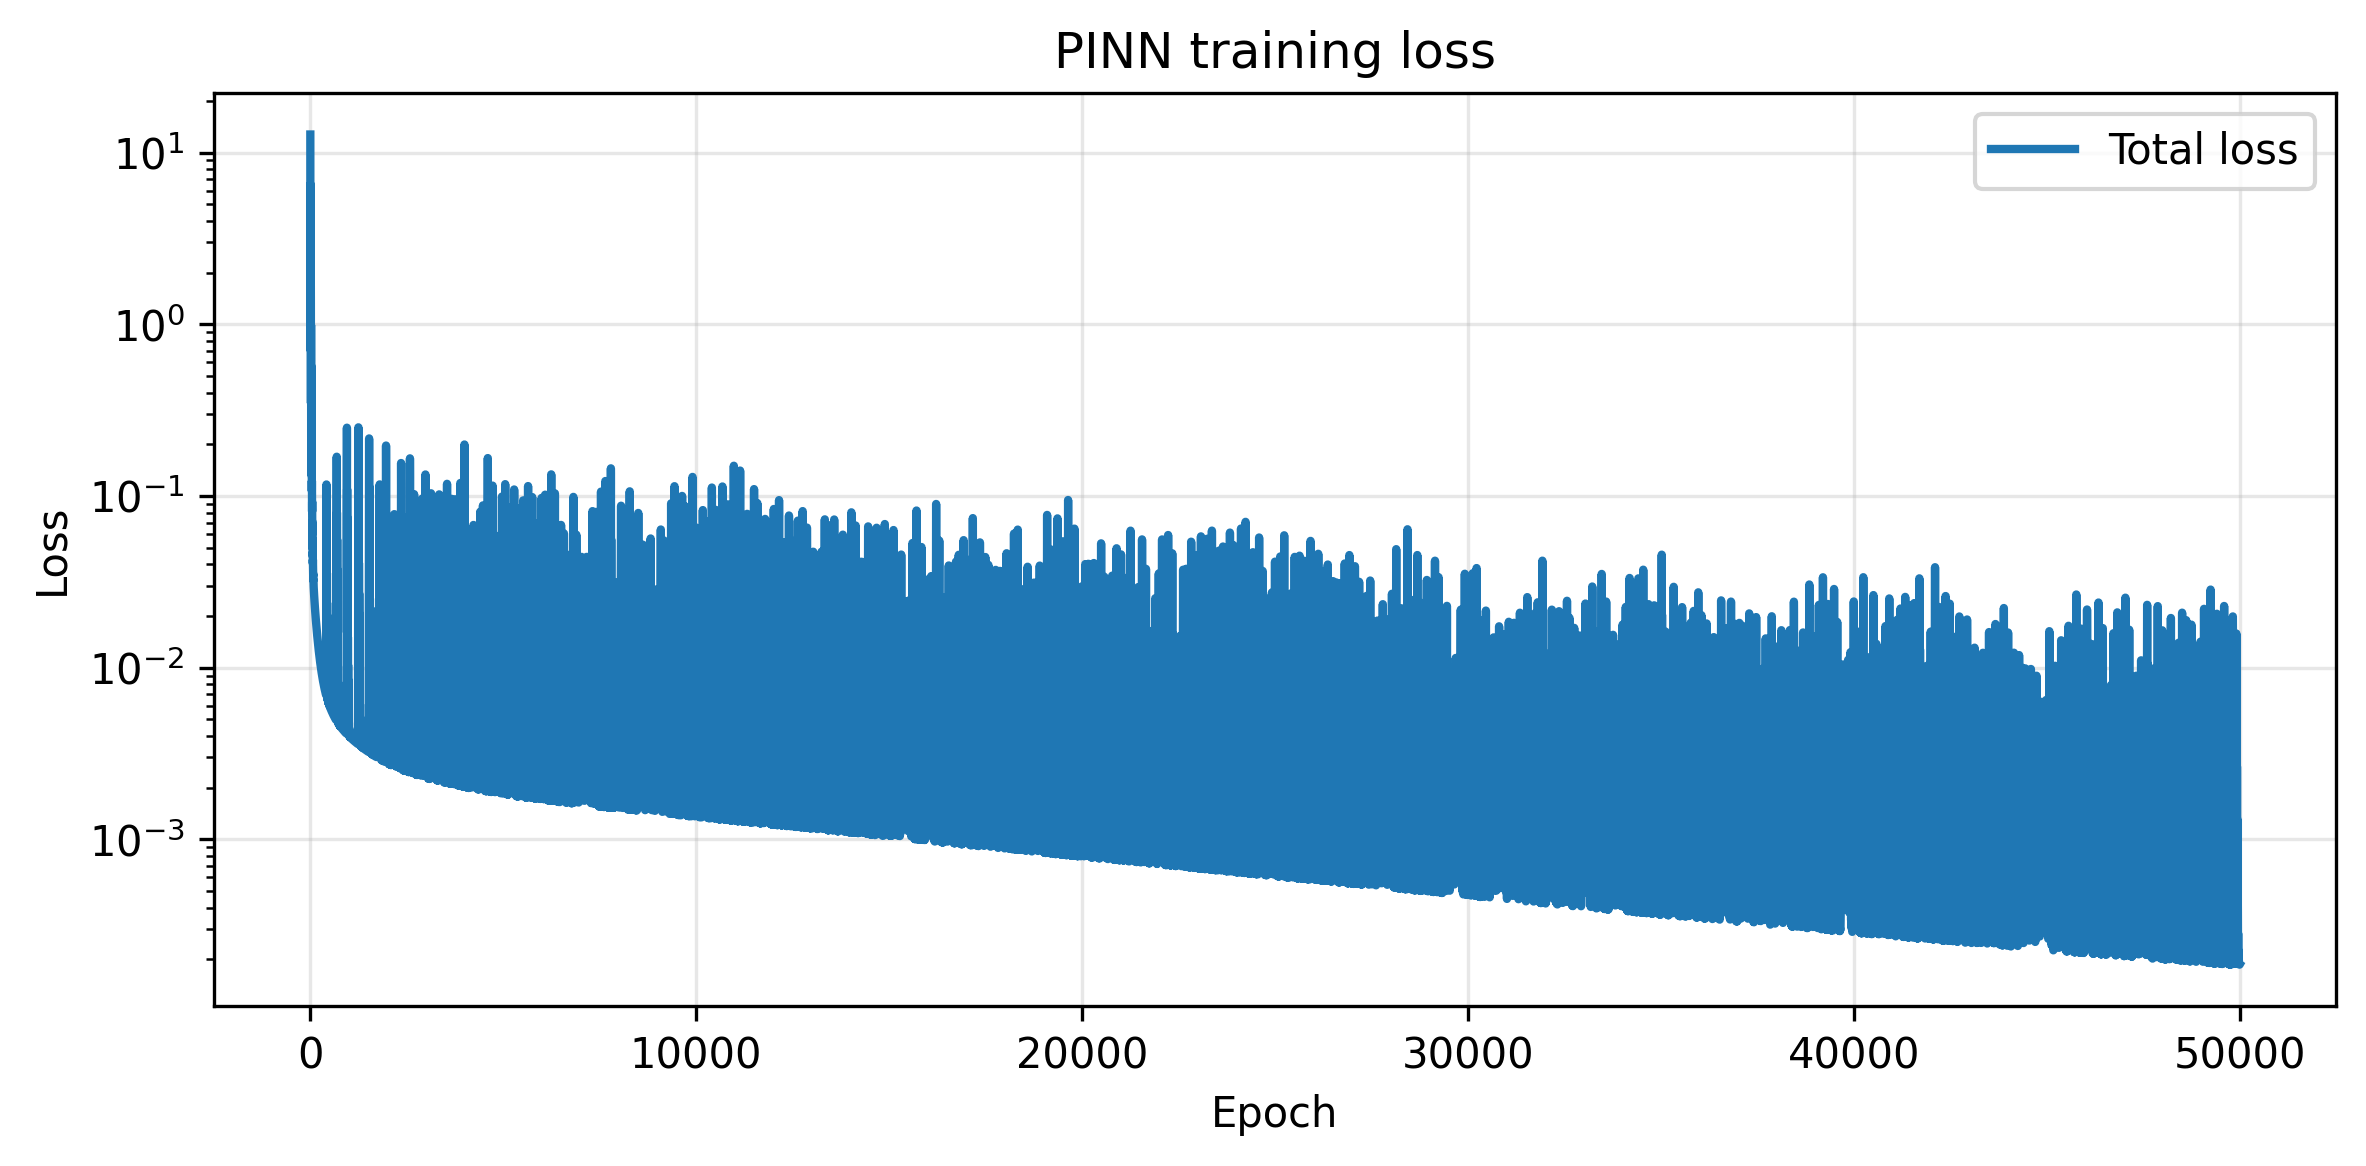
\includegraphics[width=0.78\linewidth]{problem_1_figures/problem1_20260315_203703_full_data_seed1234/training_loss.png}
    \caption{Data-assisted PINN training loss. The total loss is larger than in the physics-only case because the objective now includes a strong supervised term.}
\end{figure}

\begin{figure}[H]
    \centering
    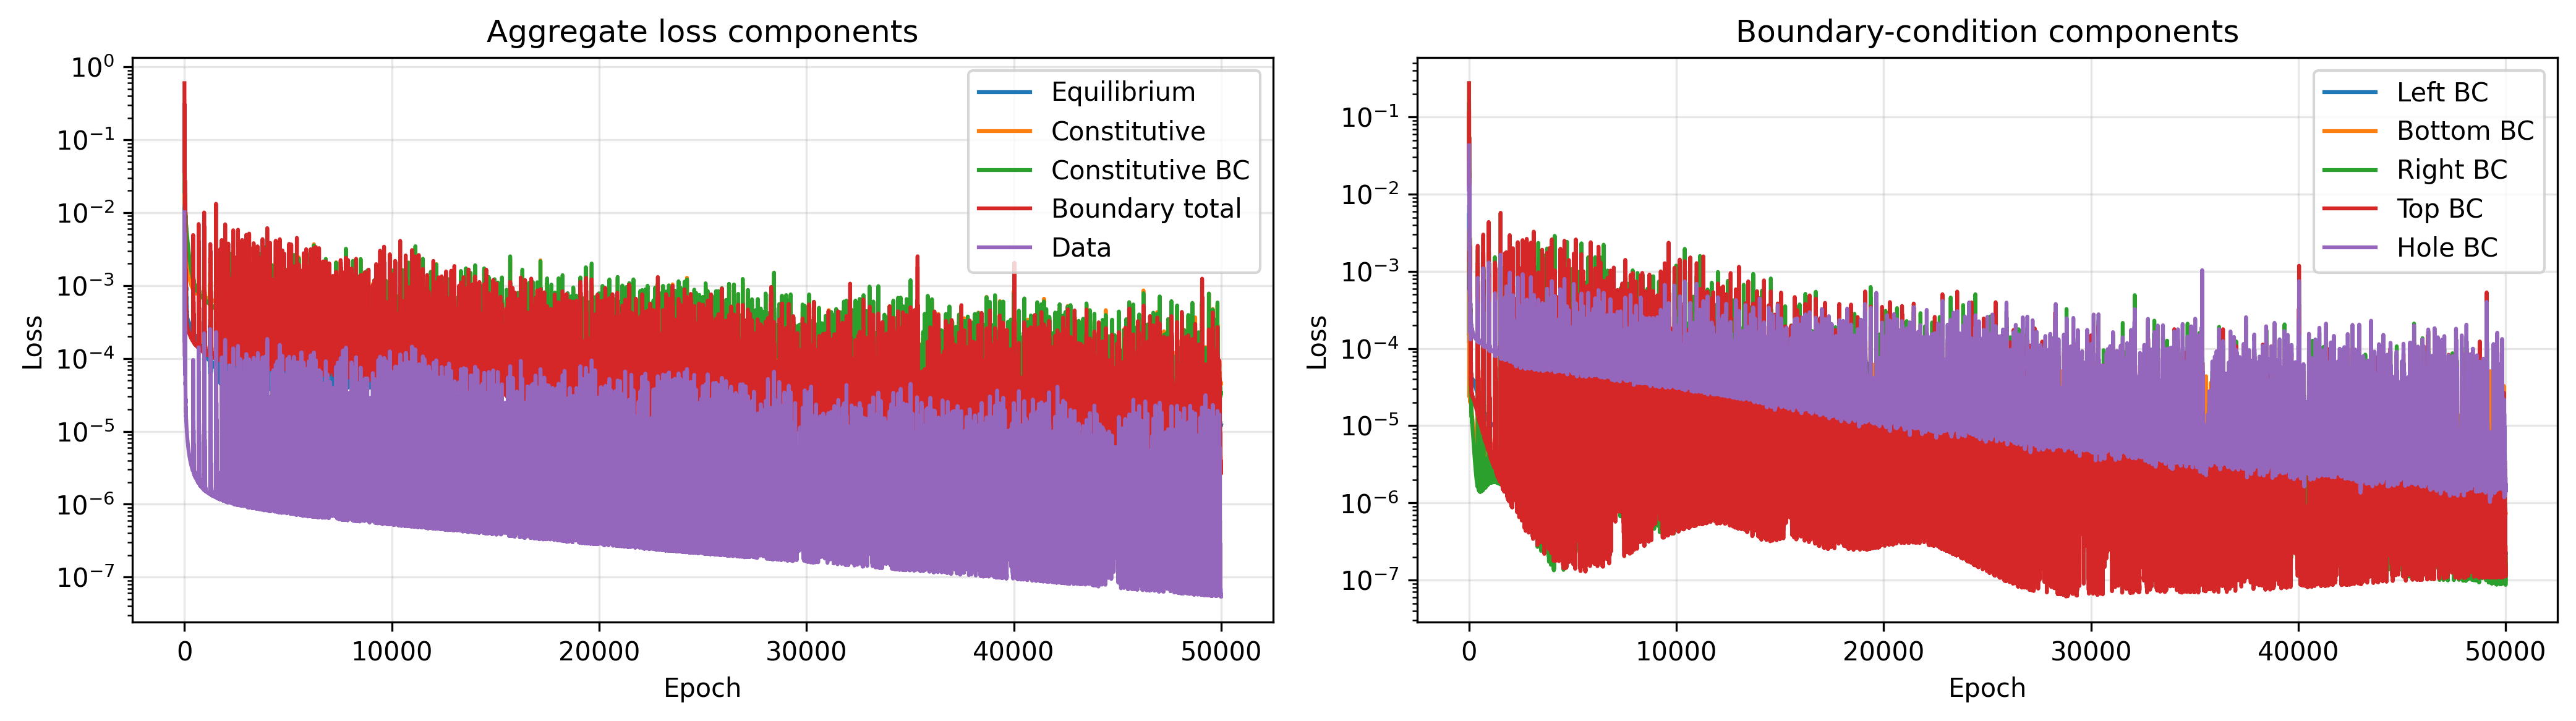
\includegraphics[width=0.78\linewidth]{problem_1_figures/problem1_20260315_203703_full_data_seed1234/loss_components.png}
    \caption{Data-assisted PINN loss components. The presence of the data term changes the optimization balance and makes the loss more aligned with FEM accuracy.}
\end{figure}

\begin{figure}[H]
    \centering
    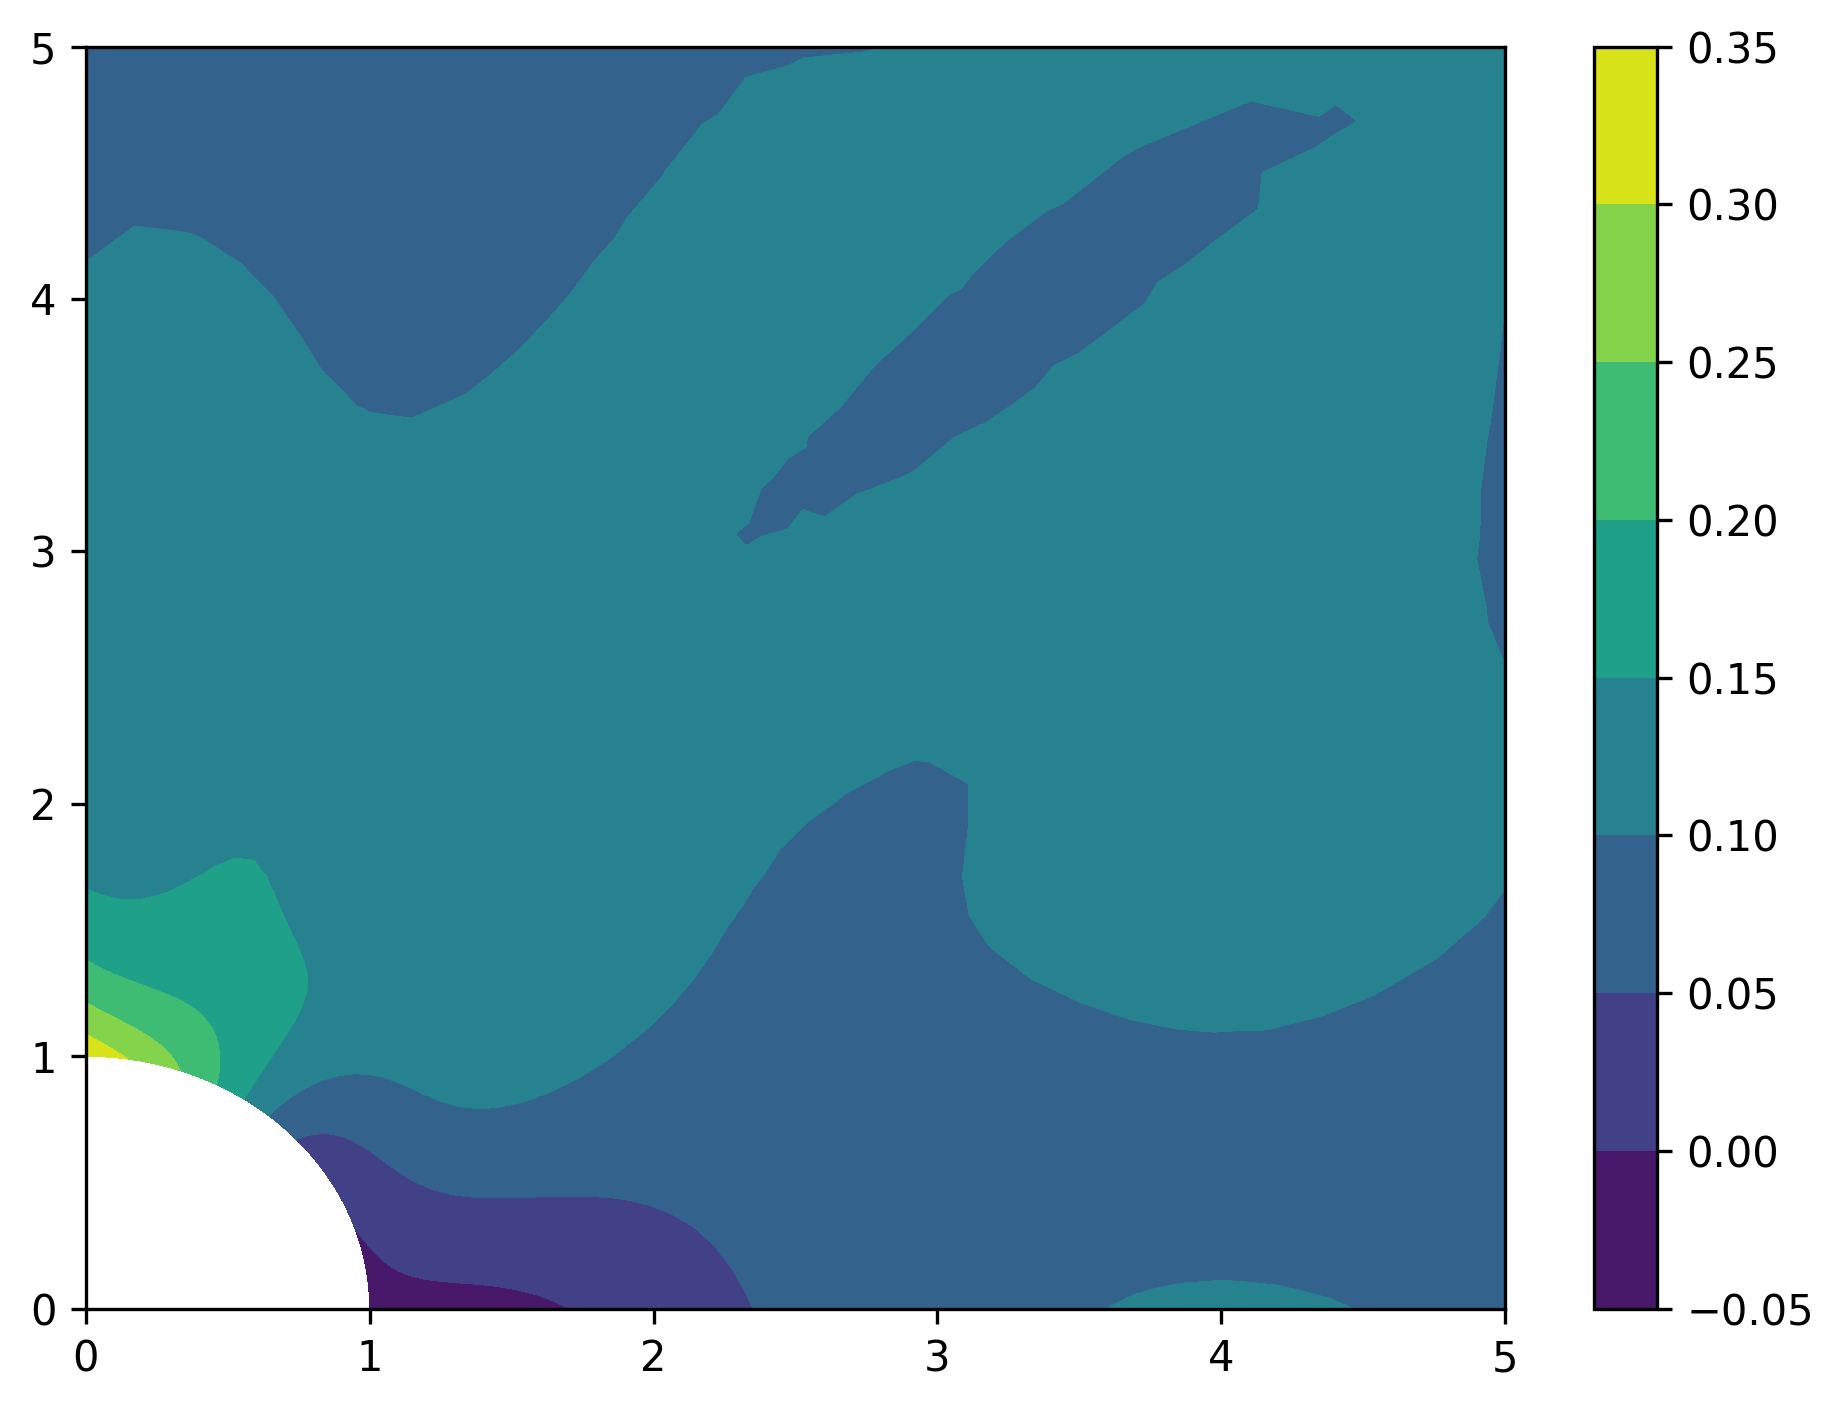
\includegraphics[width=0.72\linewidth]{problem_1_figures/problem1_20260315_203703_full_data_seed1234/stress_sigma11.png}
    \caption{Data-assisted tensile stress field \(\sigma_{11}\). The stress concentration around the hole is much more convincing visually and quantitatively than in the physics-only case.}
\end{figure}

\begin{figure}[H]
    \centering
    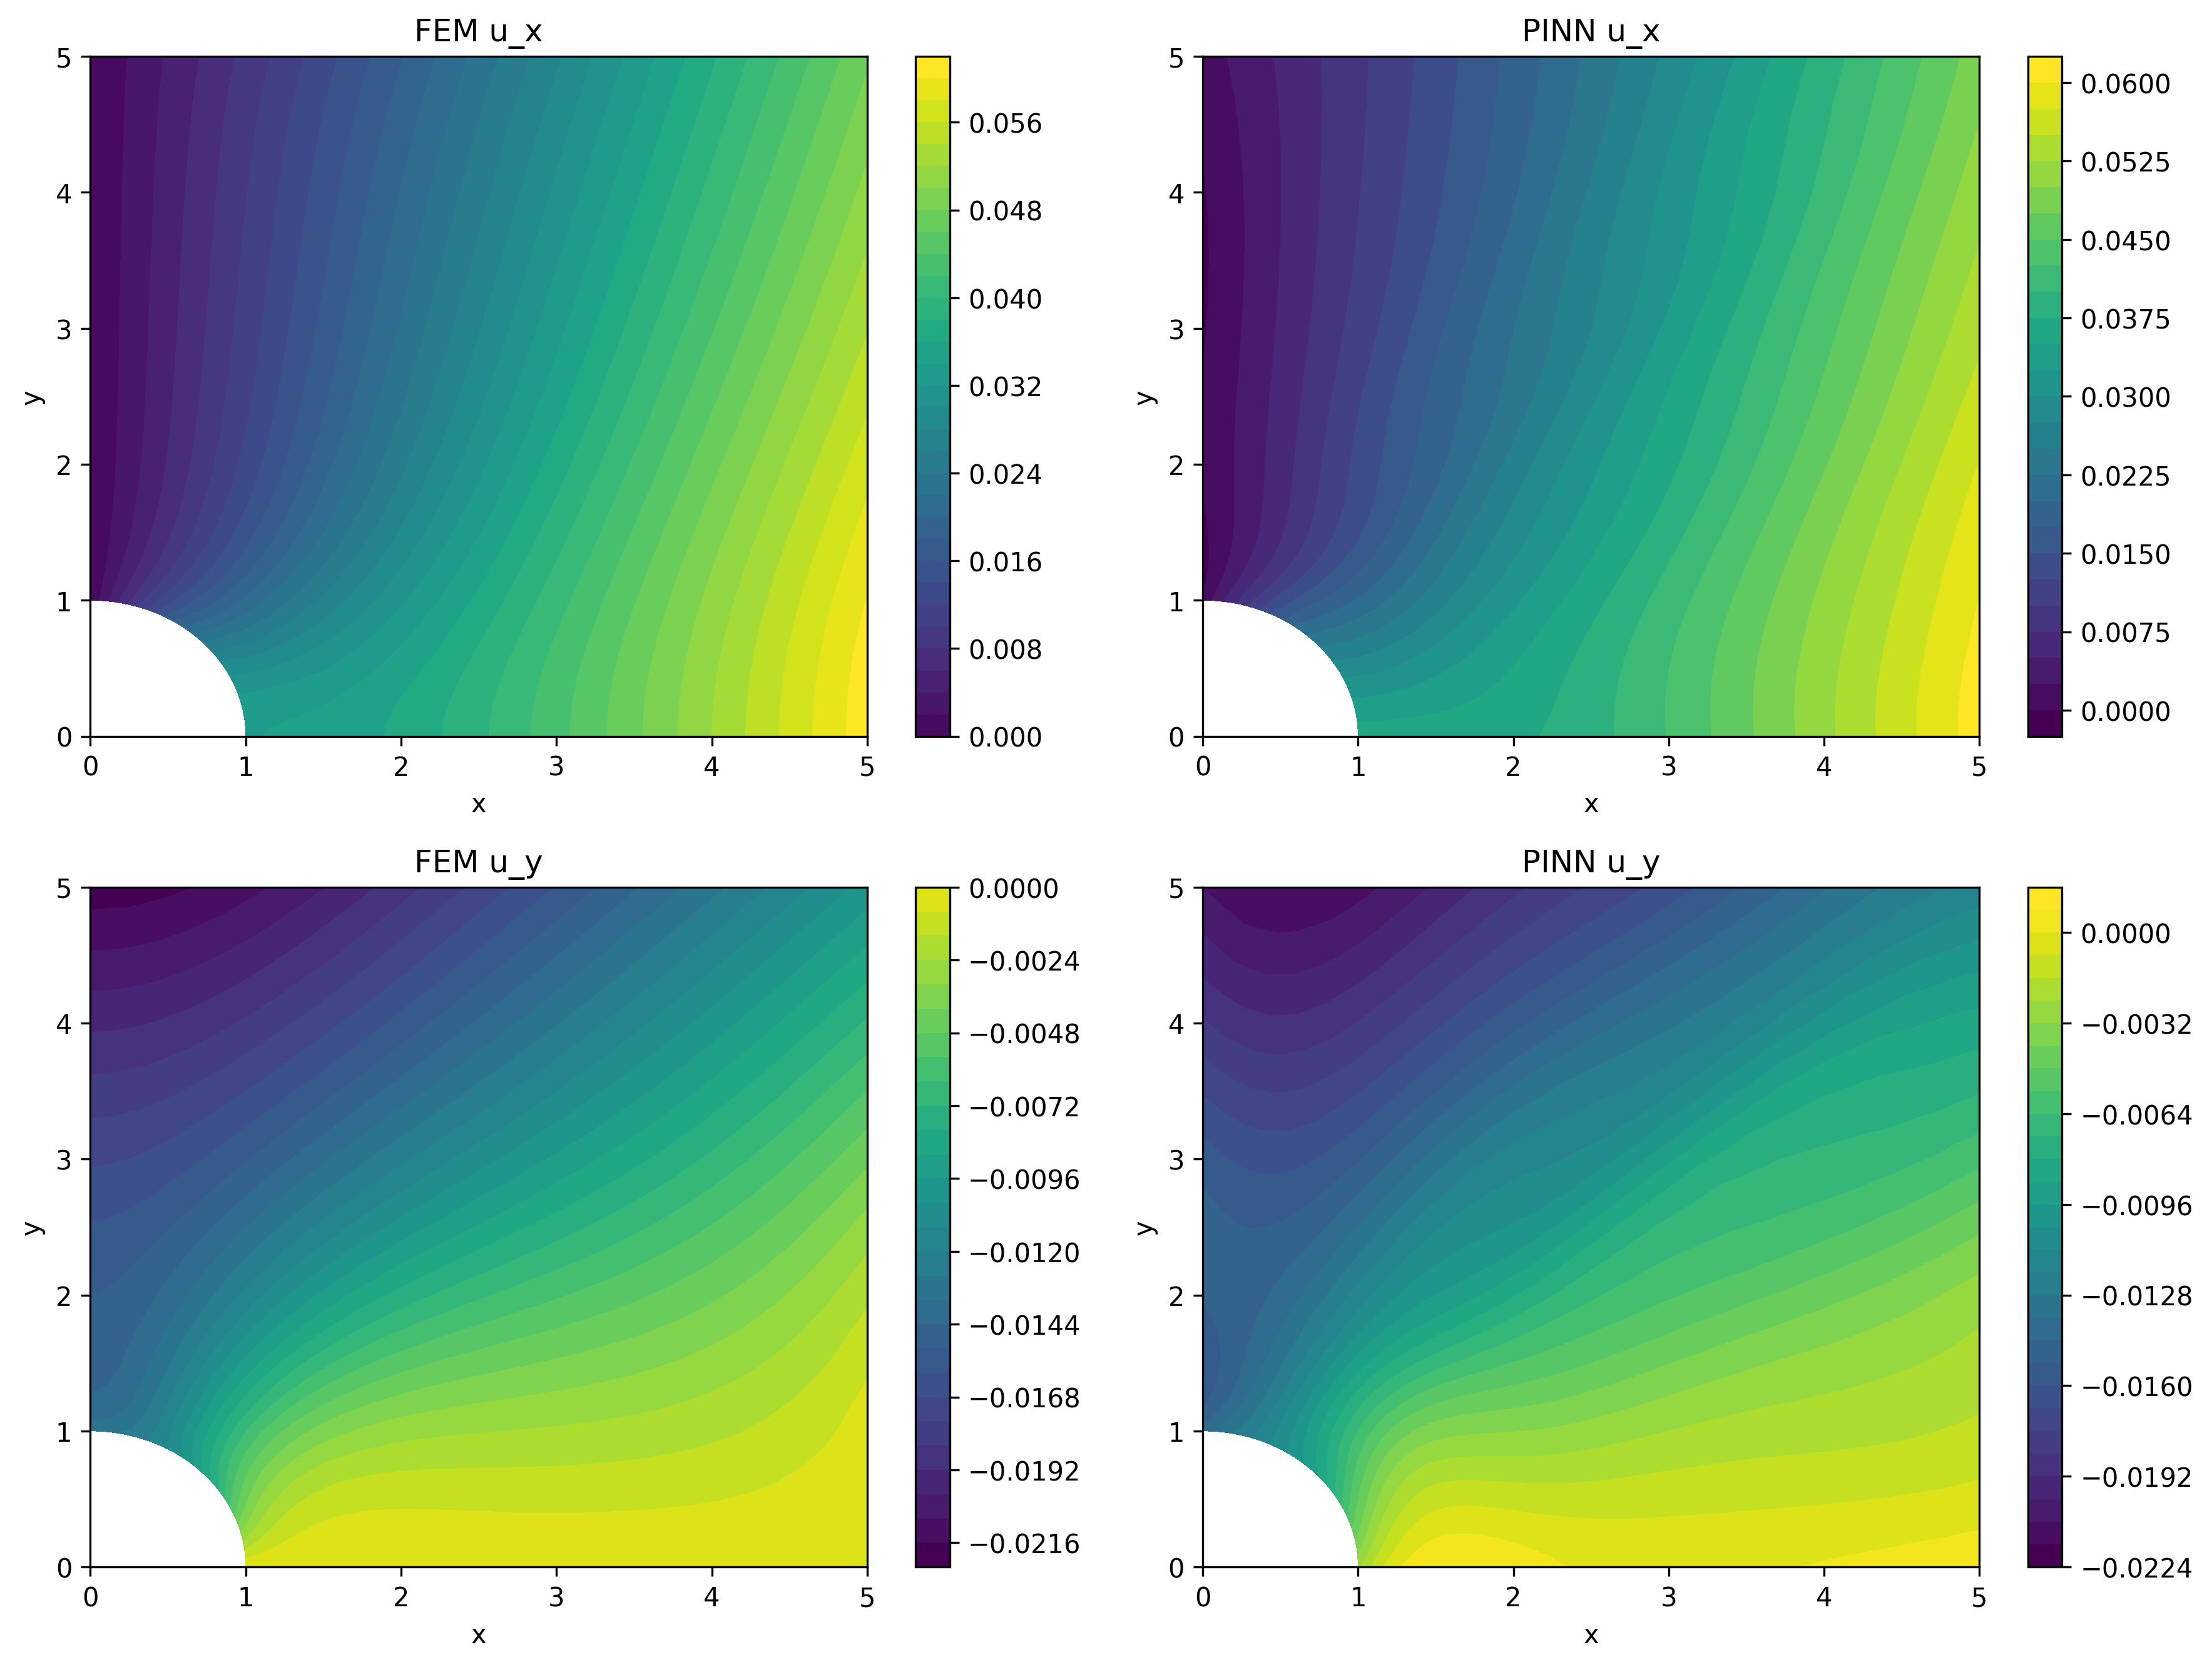
\includegraphics[width=\linewidth]{problem_1_figures/problem1_20260315_203703_full_data_seed1234/fem_vs_pinn_displacement.png}
    \caption{Data-assisted FEM-vs-PINN displacement comparison. The field now agrees closely with the FEM solution, and the error becomes much smaller and more localized.}
\end{figure}

\begin{figure}[H]
    \centering
    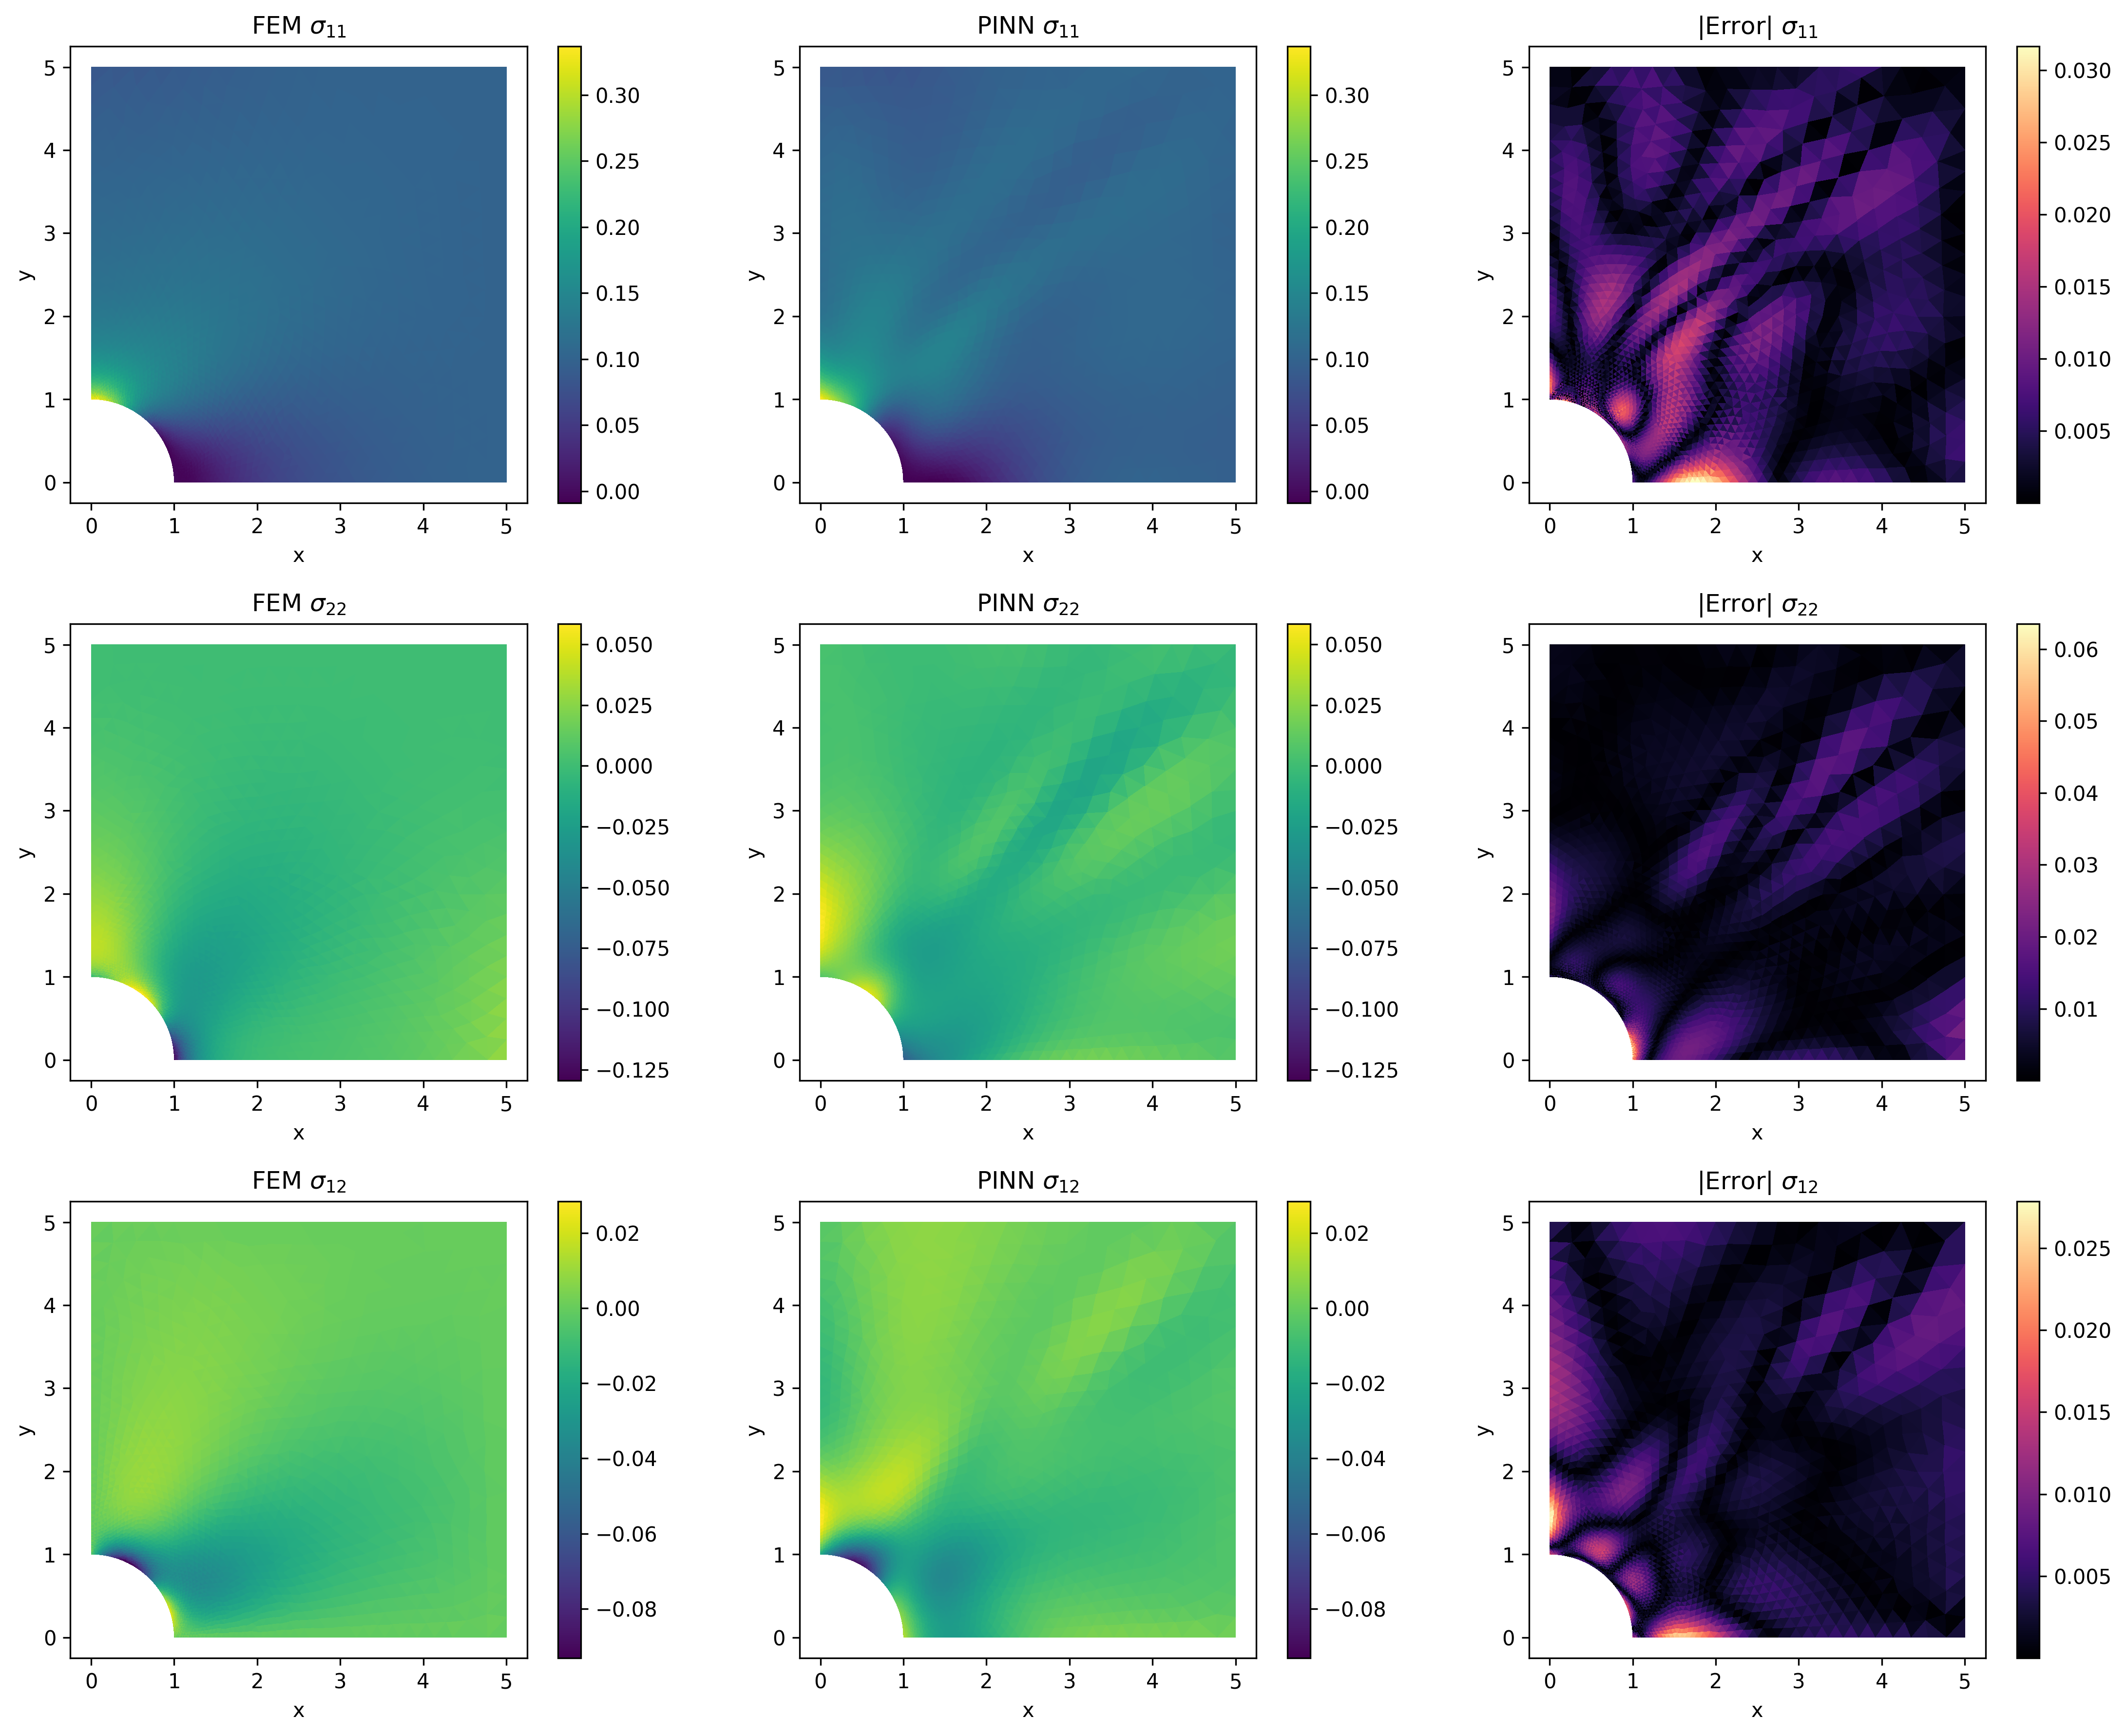
\includegraphics[width=\linewidth]{problem_1_figures/problem1_20260315_203703_full_data_seed1234/fem_vs_pinn_stress_components.png}
    \caption{Data-assisted FEM-vs-PINN stress comparison. The \(\sigma_{11}\) component is now captured well, while \(\sigma_{22}\) remains the hardest component.}
\end{figure}

\begin{figure}[H]
    \centering
    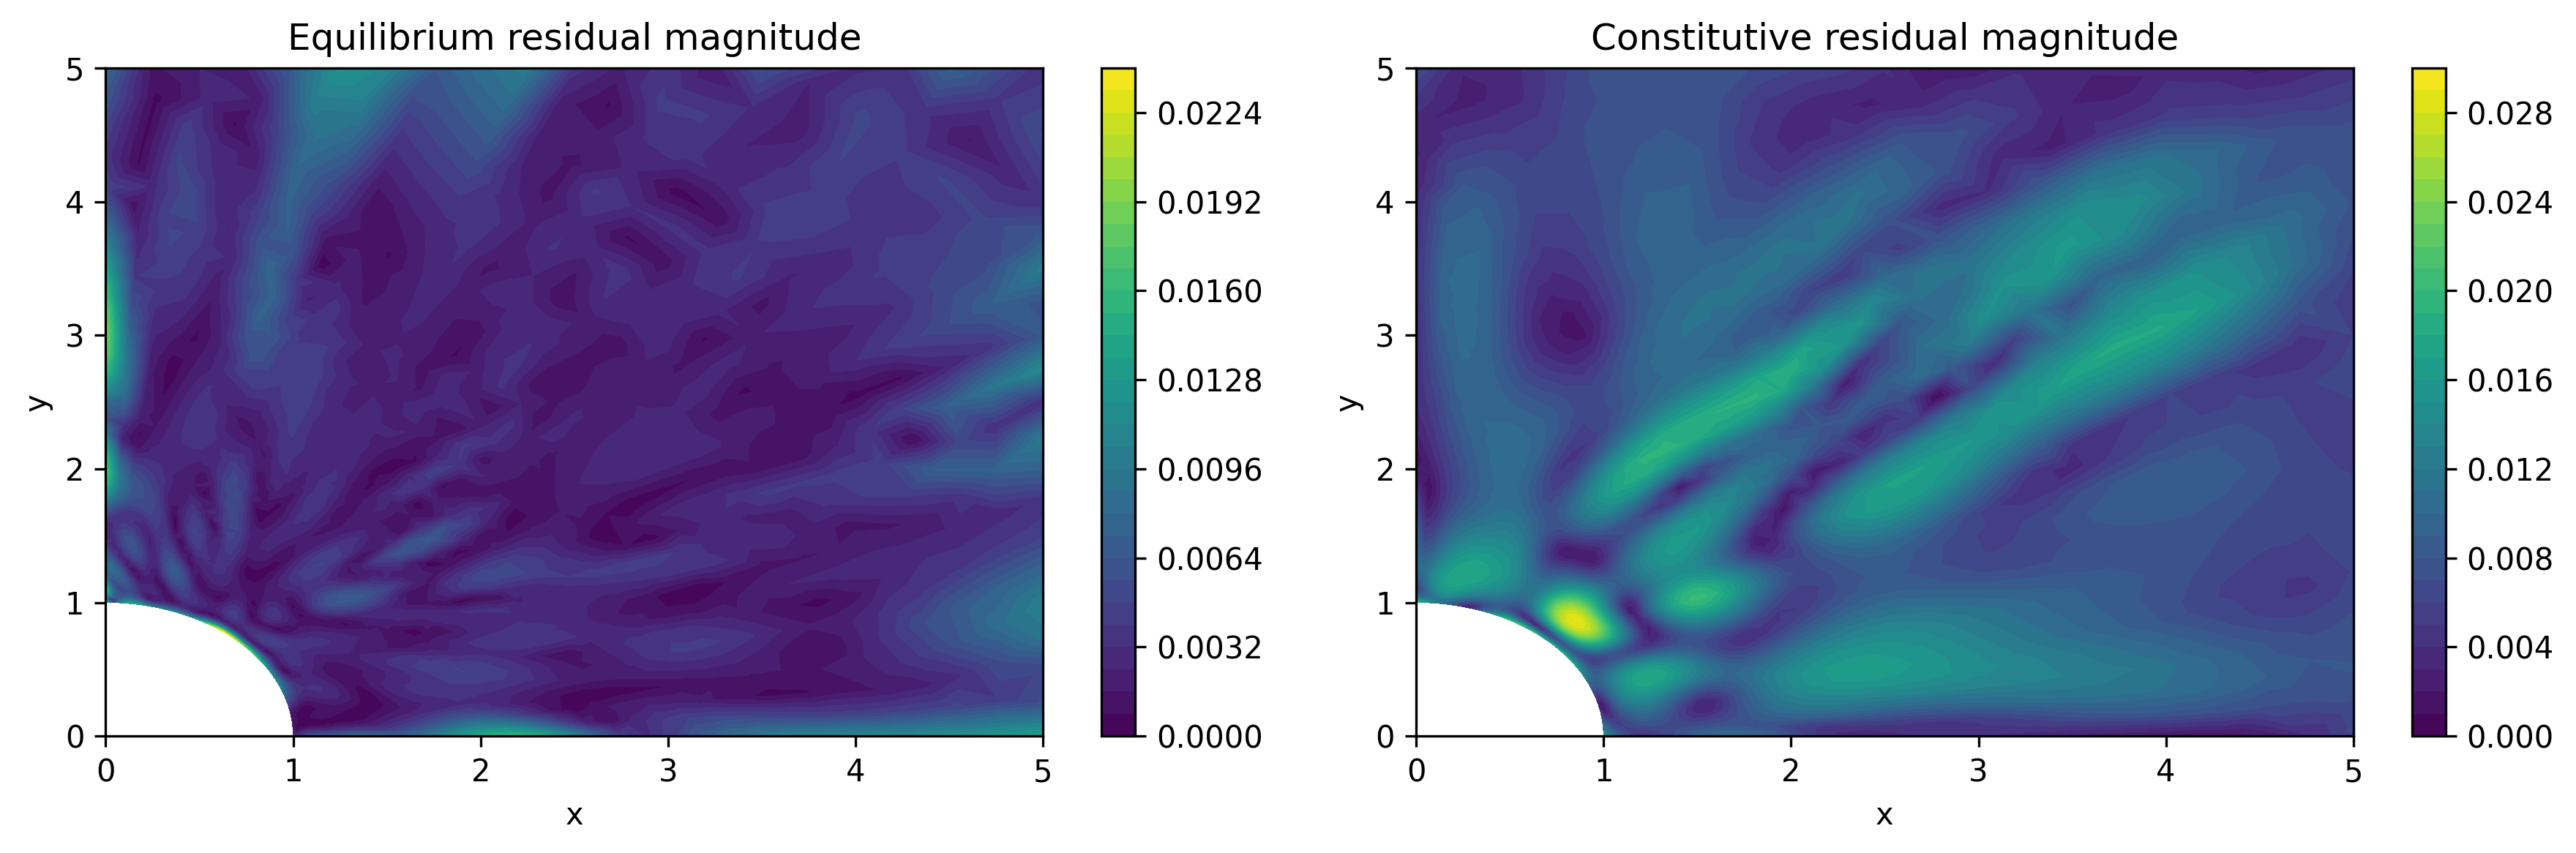
\includegraphics[width=0.9\linewidth]{problem_1_figures/problem1_20260315_203703_full_data_seed1234/residual_spatial_maps.png}
    \caption{Data-assisted residual spatial maps. The difficult region is still near the hole, but the overall residual level and the external FEM error are much smaller than in the physics-only run.}
\end{figure}

The central result of part (e) is therefore very clear: adding only 50 displacement measurements transformed the quality of the final solution. This happened because the extra supervised data anchored the displacement field and reduced the ambiguity left by the residual-only objective. Once the displacement field became much more accurate, the stress field improved as well through the constitutive coupling.

\subsection*{(f) Stress-Field Interpretation and Overall Problem 1 Discussion}

The stress-field plots are especially important for understanding the difference between the two PINN variants. In both cases, the learned \(\sigma_{11}\) field forms a concentration around the hole, so a purely qualitative glance might suggest that both models are successful. The FEM comparison shows that this would be a mistake. In the physics-only case, the broad pattern is plausible but the detailed stress distribution is still inaccurate. In the data-assisted case, both the qualitative shape and the quantitative stress errors improve substantially.

This leads to the main lesson of Problem 1:
\begin{quote}
low internal PINN residual is not sufficient; a small amount of supervised displacement data can dramatically improve the physical accuracy of the solution.
\end{quote}

The precision and device experiments reinforce that lesson. Float32/MPS was highly valuable for screening and reduced run time by roughly a factor of three in the tuning phase. However, the float32-vs-float64 rerun comparisons showed that rankings and absolute errors could shift materially, so the final defensible FEM comparisons were produced in float64 on CPU.

\subsection*{Problem 1 Improvements}

If more time and compute were available, the most useful improvements would be:
\begin{itemize}[itemsep=0.25em]
    \item tune on budgets much closer to the final 50k--100k epoch regime,
    \item use a composite tuning objective incorporating both displacement and stress accuracy,
    \item tune loss weights more systematically,
    \item test a two-stage optimizer such as Adam followed by L-BFGS,
    \item improve collocation and measurement-point sampling,
    \item make checkpoint selection more explicitly tied to the final evaluation metric,
    \item deepen the local analysis around the stress concentration zone near the hole.
\end{itemize}

These ideas are discussed further in \path{problem_1_improvements.md}, but the current workflow was already sufficient to demonstrate both the limitations of the baseline PINN and the benefits of adding small amounts of measured data.

\subsection*{Problem 1 Conclusion}

Problem 1 showed that a physics-only PINN can reach extremely low residual loss while still failing to match the FEM solution accurately. Adding 50 displacement measurements transformed the result, reducing both displacement and stress errors by large margins. The data-assisted PINN is therefore the defensible final result for this problem.

\clearpage

\section{Problem 2: Learning the Darcy Solution Operator}

\subsection*{Problem 2 Introduction}

Problem 2 is a supervised operator-learning problem. The aim is to learn the mapping from a spatially varying diffusion coefficient field \(a(x)\) to the corresponding Darcy solution field \(u(x)\). Three neural architectures were studied:
\begin{itemize}[itemsep=0.25em]
    \item a simple CNN,
    \item a U-Net,
    \item a Fourier Neural Operator.
\end{itemize}

The main interest here is not only which model yields the lowest test loss, but also why the different architectures behave differently on this fixed-grid elliptic PDE dataset.

\subsection*{Problem Setup and Data}

The Darcy problem is
\[
-\nabla \cdot \big(a(x)\nabla u(x)\big) = f(x), \qquad x \in (0,1)^2,
\]
with homogeneous Dirichlet boundary conditions
\[
u(x) = 0, \qquad x \in \partial(0,1)^2.
\]

The coursework provides paired coefficient fields \(a(x)\) and solution fields \(u(x)\) for training and testing. During development, an internal validation split was taken from the provided training set to choose hyperparameters. For the final reported runs, the chosen configuration for each model was retrained on the full training set and then evaluated on the provided test set.

\subsection*{(a) CNN Models: Architecture, Optimizer, and Learning Rate}

Two CNN-style models were studied.

\paragraph{Simple CNN.}
The simple CNN was implemented as an encoder-decoder with pooling, batch normalization, and upsampling, but without skip connections. This made it a meaningful baseline rather than a deliberately weak toy model. Because the Darcy solution is a smooth spatial field on a fixed grid, a convolutional model is already a natural choice.

\paragraph{U-Net.}
The U-Net used the same broad encoder-decoder idea but added skip connections from encoder to decoder blocks. These skip connections preserve finer spatial information that may otherwise be lost through downsampling. For an elliptic PDE solution, this is useful because the field is globally smooth but still contains local variation induced by the coefficient field.

Both CNN models used Adam with StepLR, and the selected final settings were:
\begin{itemize}[itemsep=0.25em]
    \item base channels = 32,
    \item learning rate = \(10^{-3}\),
    \item weight decay = \(10^{-6}\).
\end{itemize}

These settings were chosen from the internal validation runs described below.

\subsection*{(b) FNO Architecture, Optimizer, and Learning Rate}

The FNO was implemented using spectral convolution layers, pointwise linear layers, and Fourier-mode truncation. Conceptually, this architecture is attractive because operator learning often depends on global structure as much as local detail. The FNO can therefore capture long-range interactions more directly than a purely local convolutional model.

The final selected FNO settings were:
\begin{itemize}[itemsep=0.25em]
    \item modes = 8,
    \item width = 32,
    \item learning rate = \(5\times10^{-4}\),
    \item weight decay = \(10^{-6}\).
\end{itemize}

The optimizer was again Adam with StepLR.

\subsection*{Hyperparameter Tuning Strategy}

Problem 2 used manual grid search rather than Optuna. The tuning process was deliberately straightforward: define a small search space, evaluate validation performance, and then retrain the winning configuration on the full training set.

For the simple CNN and U-Net, the search space was:

\begin{table}[H]
\centering
\begin{tabular}{ll}
\toprule
Hyperparameter & Search space \\
\midrule
base channels & 16, 32 \\
learning rate & \(10^{-3}\), \(5\times10^{-4}\) \\
weight decay & 0, \(10^{-6}\) \\
\bottomrule
\end{tabular}
\caption{Manual grid-search space for the simple CNN and U-Net.}
\end{table}

For the FNO, the search space was:

\begin{table}[H]
\centering
\begin{tabular}{ll}
\toprule
Hyperparameter & Search space \\
\midrule
modes & 8, 12 \\
width & 24, 32 \\
learning rate & \(10^{-3}\), \(5\times10^{-4}\) \\
\bottomrule
\end{tabular}
\caption{Manual grid-search space for the FNO.}
\end{table}

The selected final settings were:
\begin{itemize}[itemsep=0.25em]
    \item \textbf{Simple CNN}: base channels 32, learning rate \(10^{-3}\), weight decay \(10^{-6}\),
    \item \textbf{U-Net}: base channels 32, learning rate \(10^{-3}\), weight decay \(10^{-6}\),
    \item \textbf{FNO}: modes 8, width 32, learning rate \(5\times10^{-4}\), weight decay \(10^{-6}\).
\end{itemize}

Unlike Problem 1, there was no Optuna-based tuning here. The search was smaller, cheaper, and fully transparent.

\subsection*{Final Quantitative Comparison}

The canonical final results are summarized in Table~\ref{tab:p2final}.

\begin{table}[H]
\centering
\begin{tabular}{lrrrrr}
\toprule
Model & Epochs & Parameters & Training time & Device & Final test loss \\
\midrule
Simple CNN & 300 & 426,177 & 0:06:31 & MPS & 0.005034 \\
U-Net & 400 & 472,257 & 0:06:45 & MPS & 0.002994 \\
FNO & 500 & 541,441 & 0:50:54 & CPU & 0.000772 \\
\bottomrule
\end{tabular}
\caption{Canonical final results for the three Problem 2 models.}
\label{tab:p2final}
\end{table}

The U-Net improved on the simple CNN by about 40.5\%, while the CPU FNO improved on the U-Net by about 74.2\%. Relative to the simple CNN, the CPU FNO improved the final test loss by about 84.7\%.

\subsection*{Graphical Analysis of the Darcy Predictions}

\paragraph{Simple CNN.}

\begin{figure}[H]
    \centering
    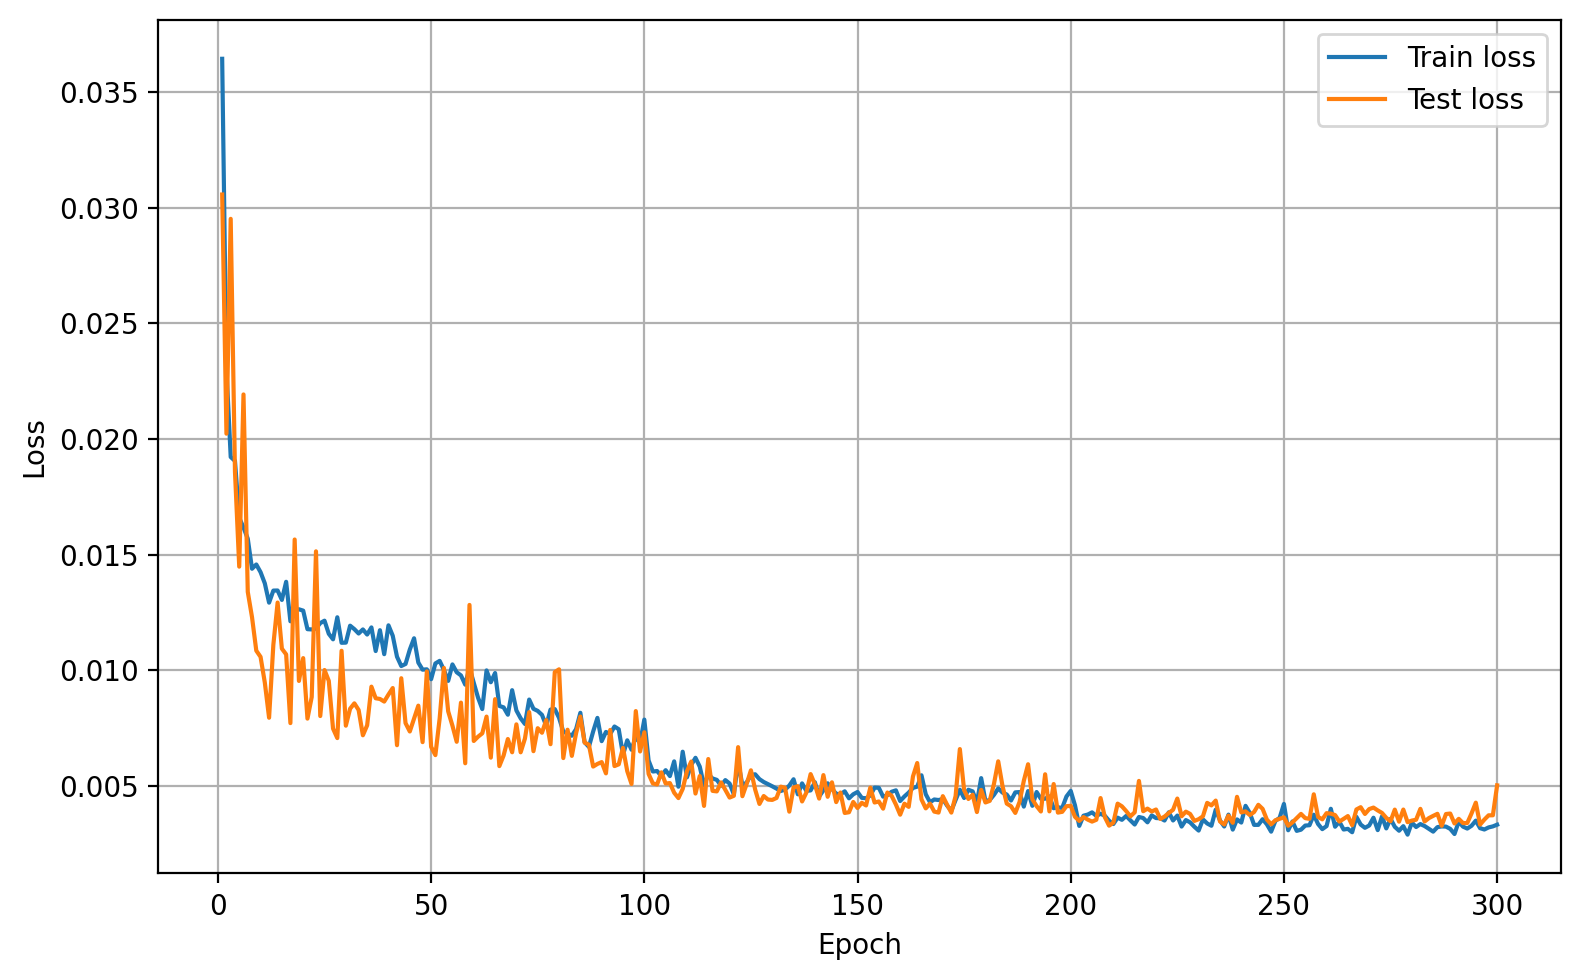
\includegraphics[width=0.78\linewidth]{problem_2_outputs/darcy_cnn_simple/20260316_114818_single_final/figures/loss_curve.png}
    \caption{Simple CNN train/test loss curve. The training behaviour is stable, and the test loss converges to a strong baseline value.}
\end{figure}

\begin{figure}[H]
    \centering
    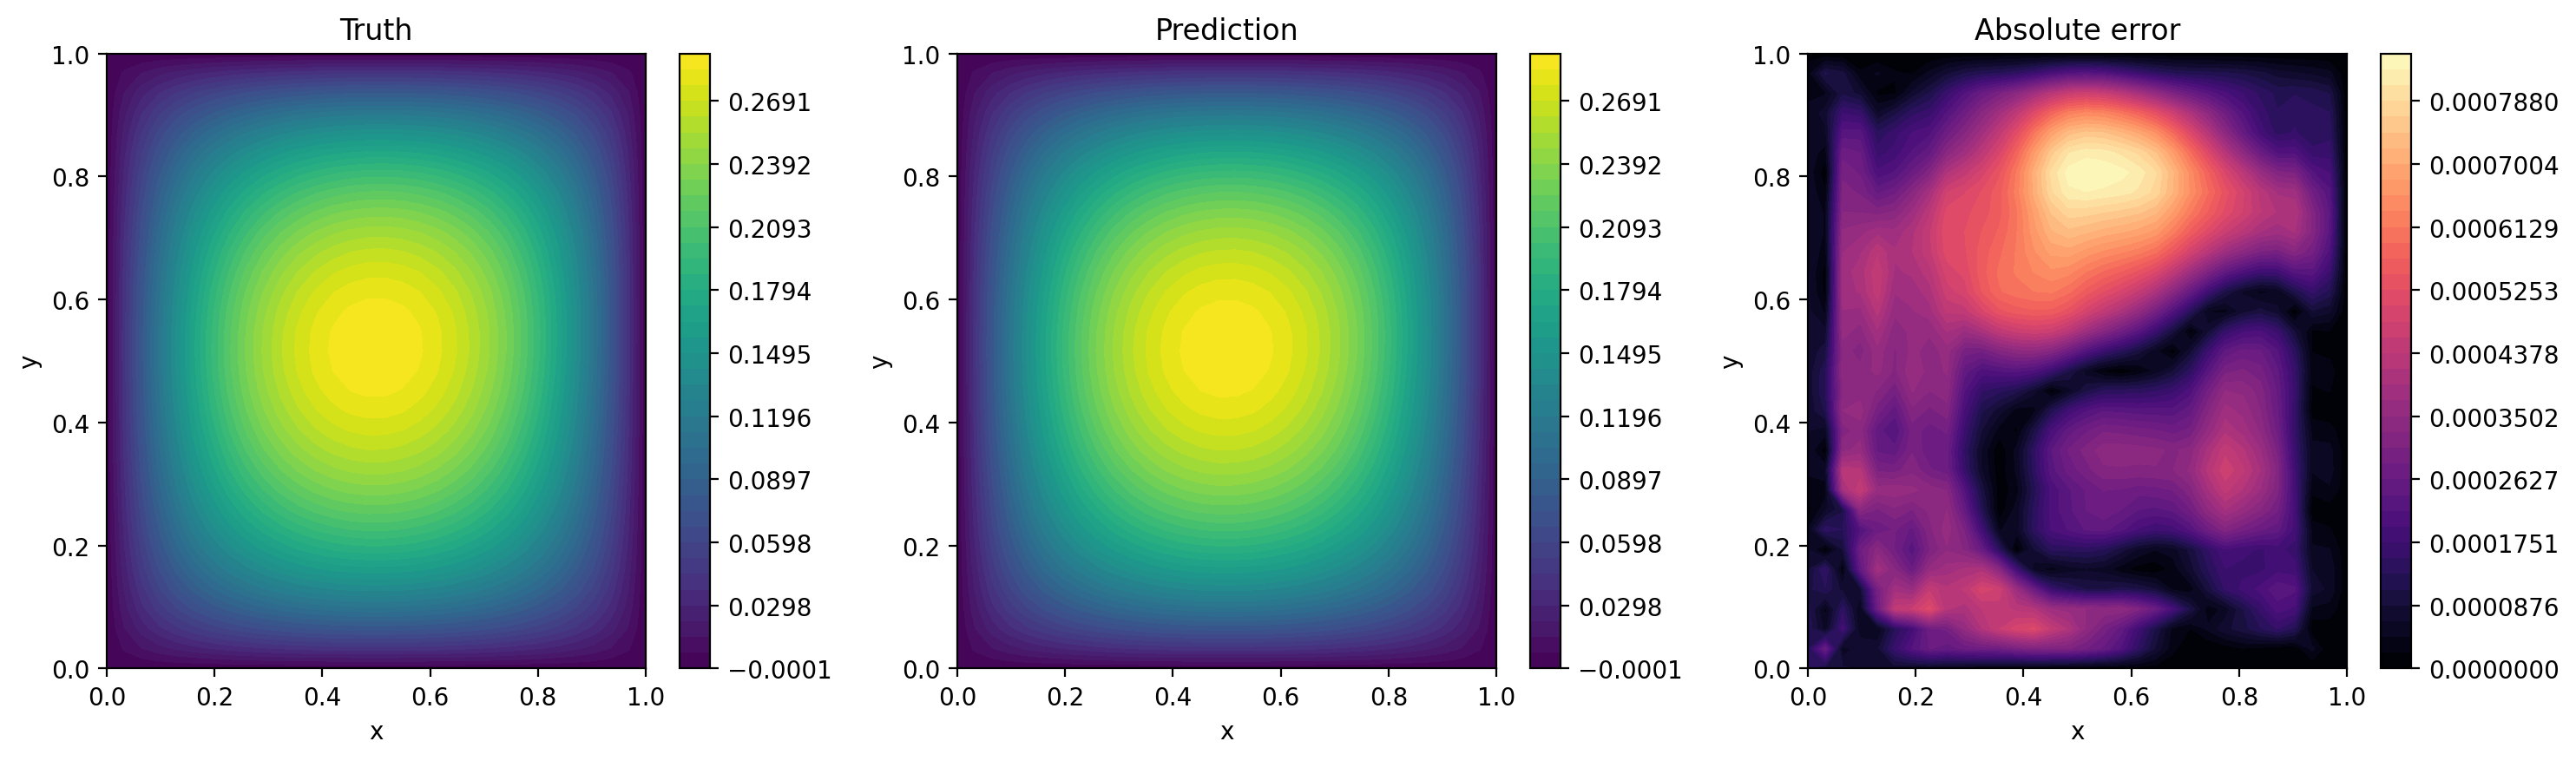
\includegraphics[width=\linewidth]{problem_2_outputs/darcy_cnn_simple/20260316_114818_single_final/figures/prediction_comparison.png}
    \caption{Simple CNN truth, prediction, and absolute error for a test sample. The global structure is captured well, but some local detail is visibly smoothed out.}
\end{figure}

The simple CNN performed very well for a baseline. This is not surprising in a fixed-grid image-to-image setting: the smooth elliptic solution field is already well matched to convolutional inductive bias. The main limitation appears in the error plot, where local detail is less sharply preserved than in the U-Net or FNO.

\paragraph{U-Net.}

\begin{figure}[H]
    \centering
    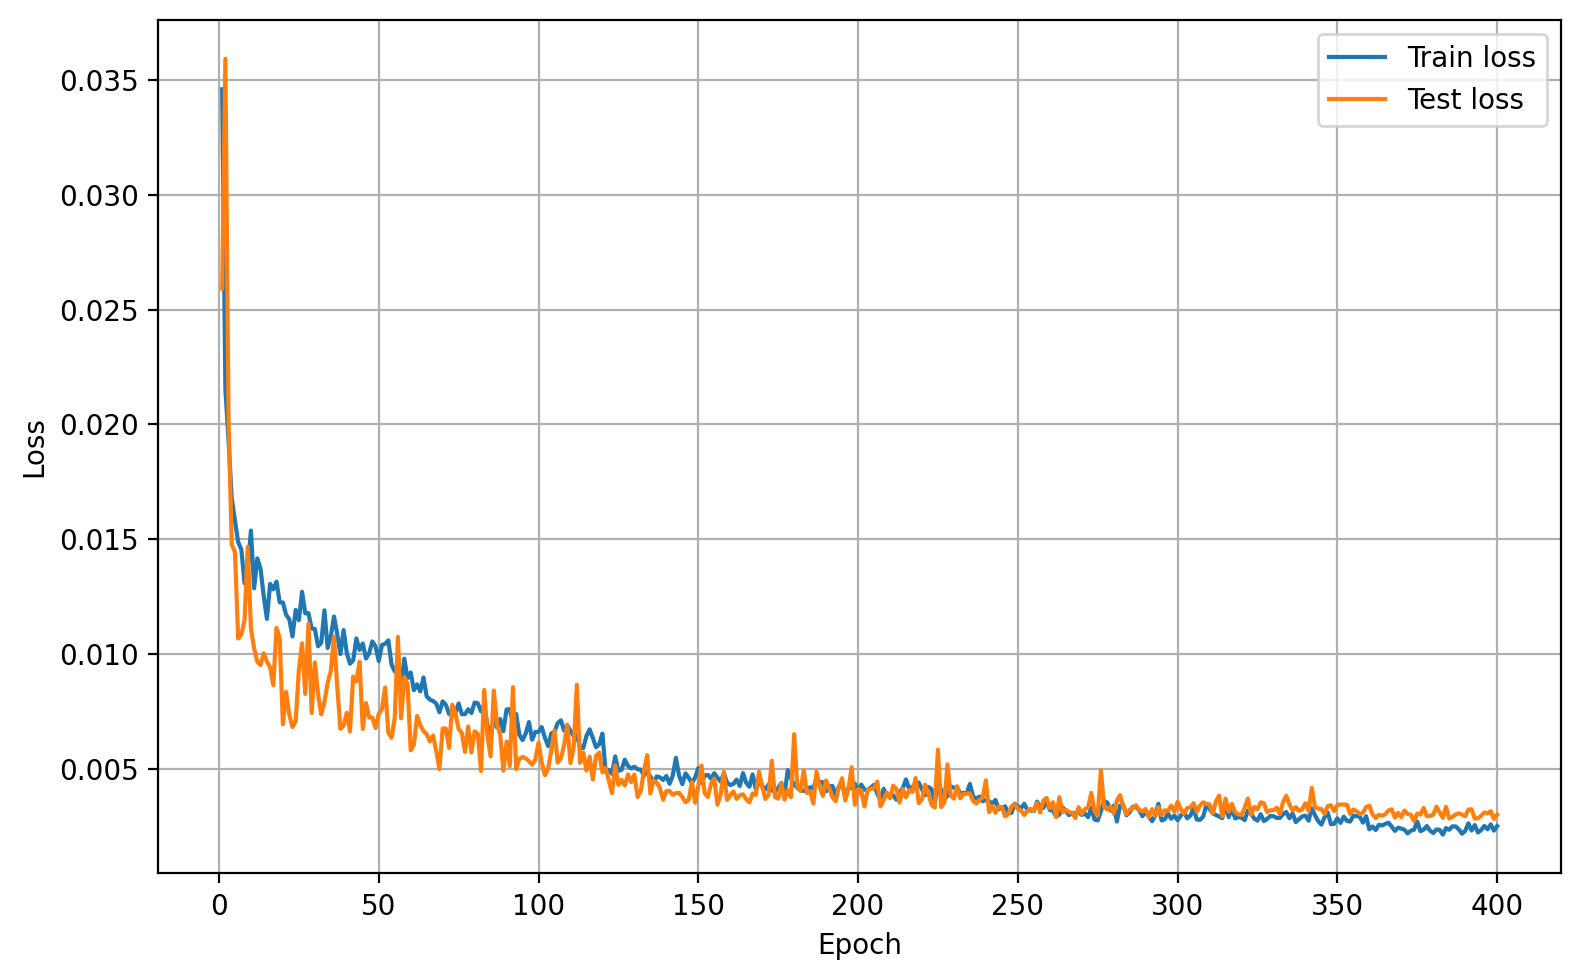
\includegraphics[width=0.78\linewidth]{problem_2_outputs/darcy_cnn_unet/20260316_115014_single_final/figures/loss_curve.png}
    \caption{U-Net train/test loss curve. The U-Net converges to a lower test loss than the simple CNN while maintaining similarly stable optimization.}
\end{figure}

\begin{figure}[H]
    \centering
    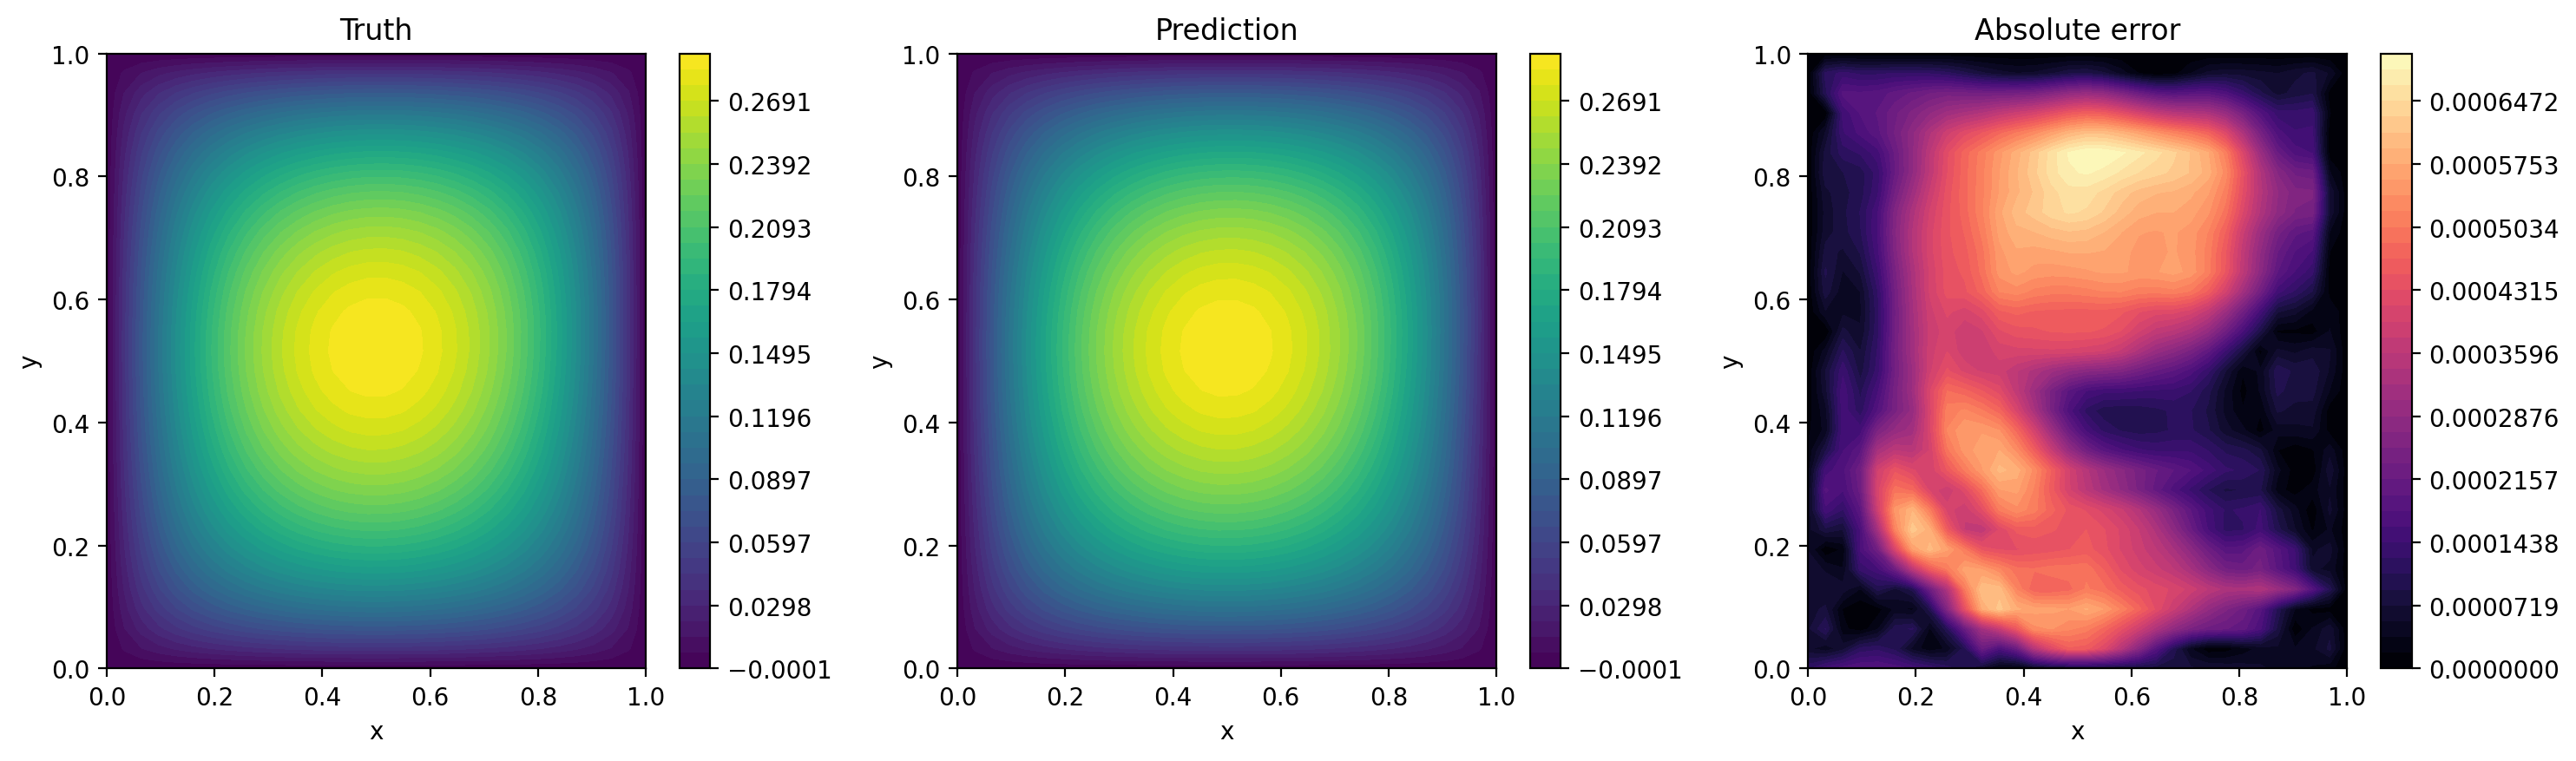
\includegraphics[width=\linewidth]{problem_2_outputs/darcy_cnn_unet/20260316_115014_single_final/figures/prediction_comparison.png}
    \caption{U-Net truth, prediction, and absolute error for a test sample. The prediction is visibly closer to the truth than for the simple CNN, and the error becomes smaller and more localized.}
\end{figure}

The U-Net behaved as expected. The skip connections preserved multiscale spatial information and reduced the error compared with the simple CNN. The improvement in test loss was not merely numerical; it was also visible in the sharper and more localized error field.

\paragraph{FNO.}

\begin{figure}[H]
    \centering
    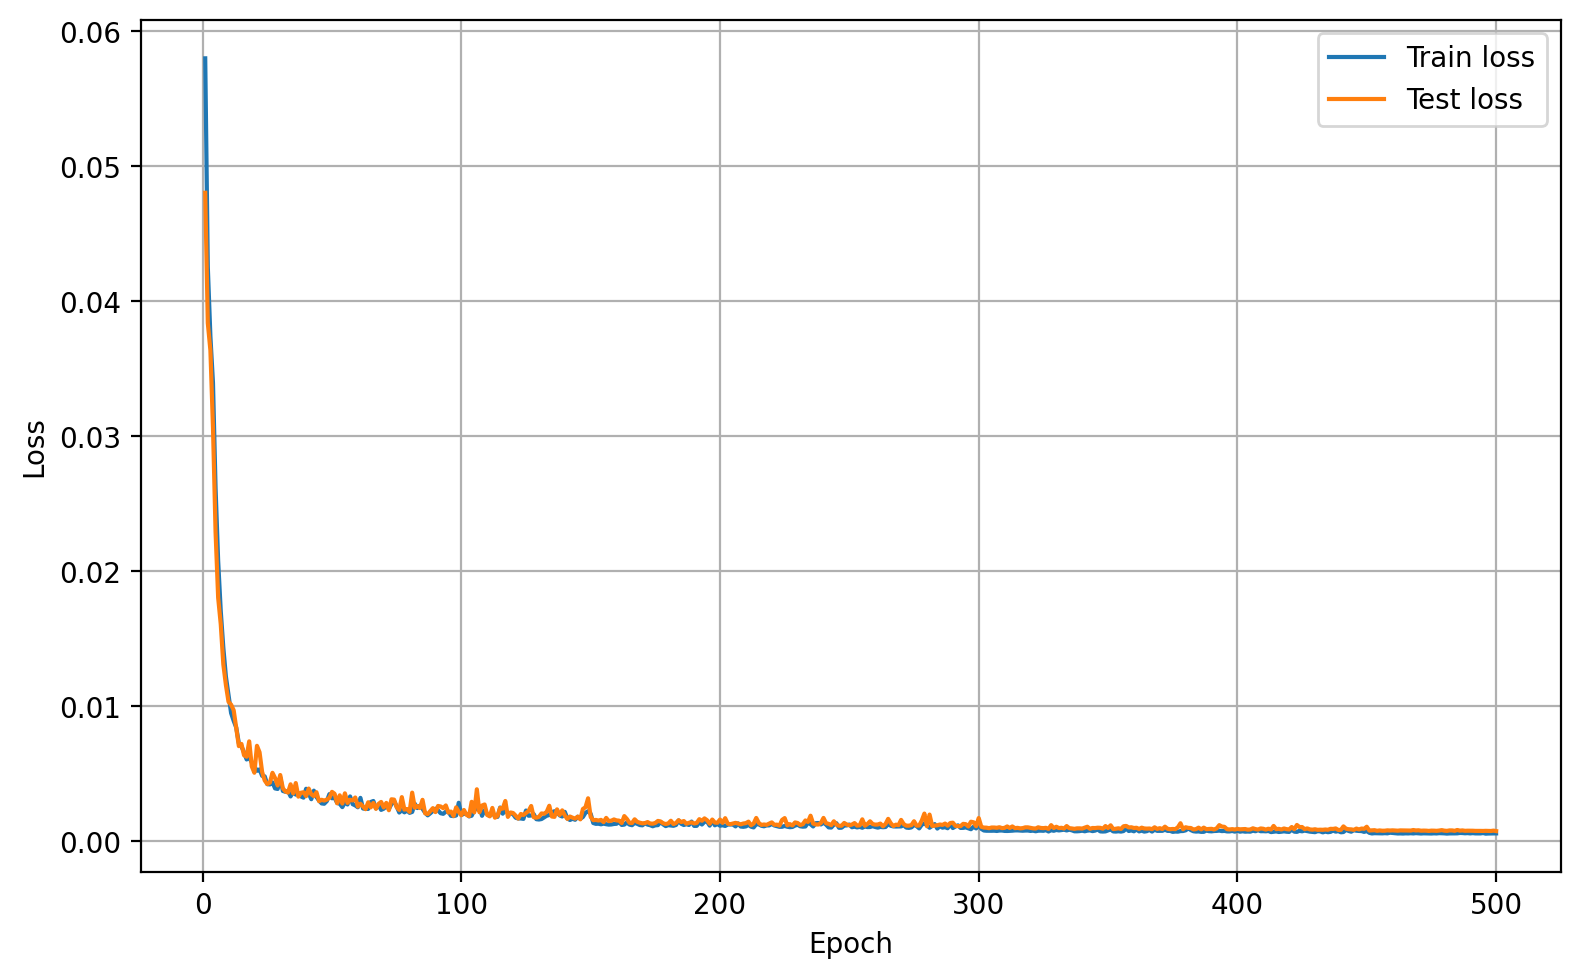
\includegraphics[width=0.78\linewidth]{problem_2_outputs/darcy_fno/20260316_124531_single_final/figures/loss_curve.png}
    \caption{CPU FNO train/test loss curve. The loss converges to a much lower value than for either CNN-based model.}
\end{figure}

\begin{figure}[H]
    \centering
    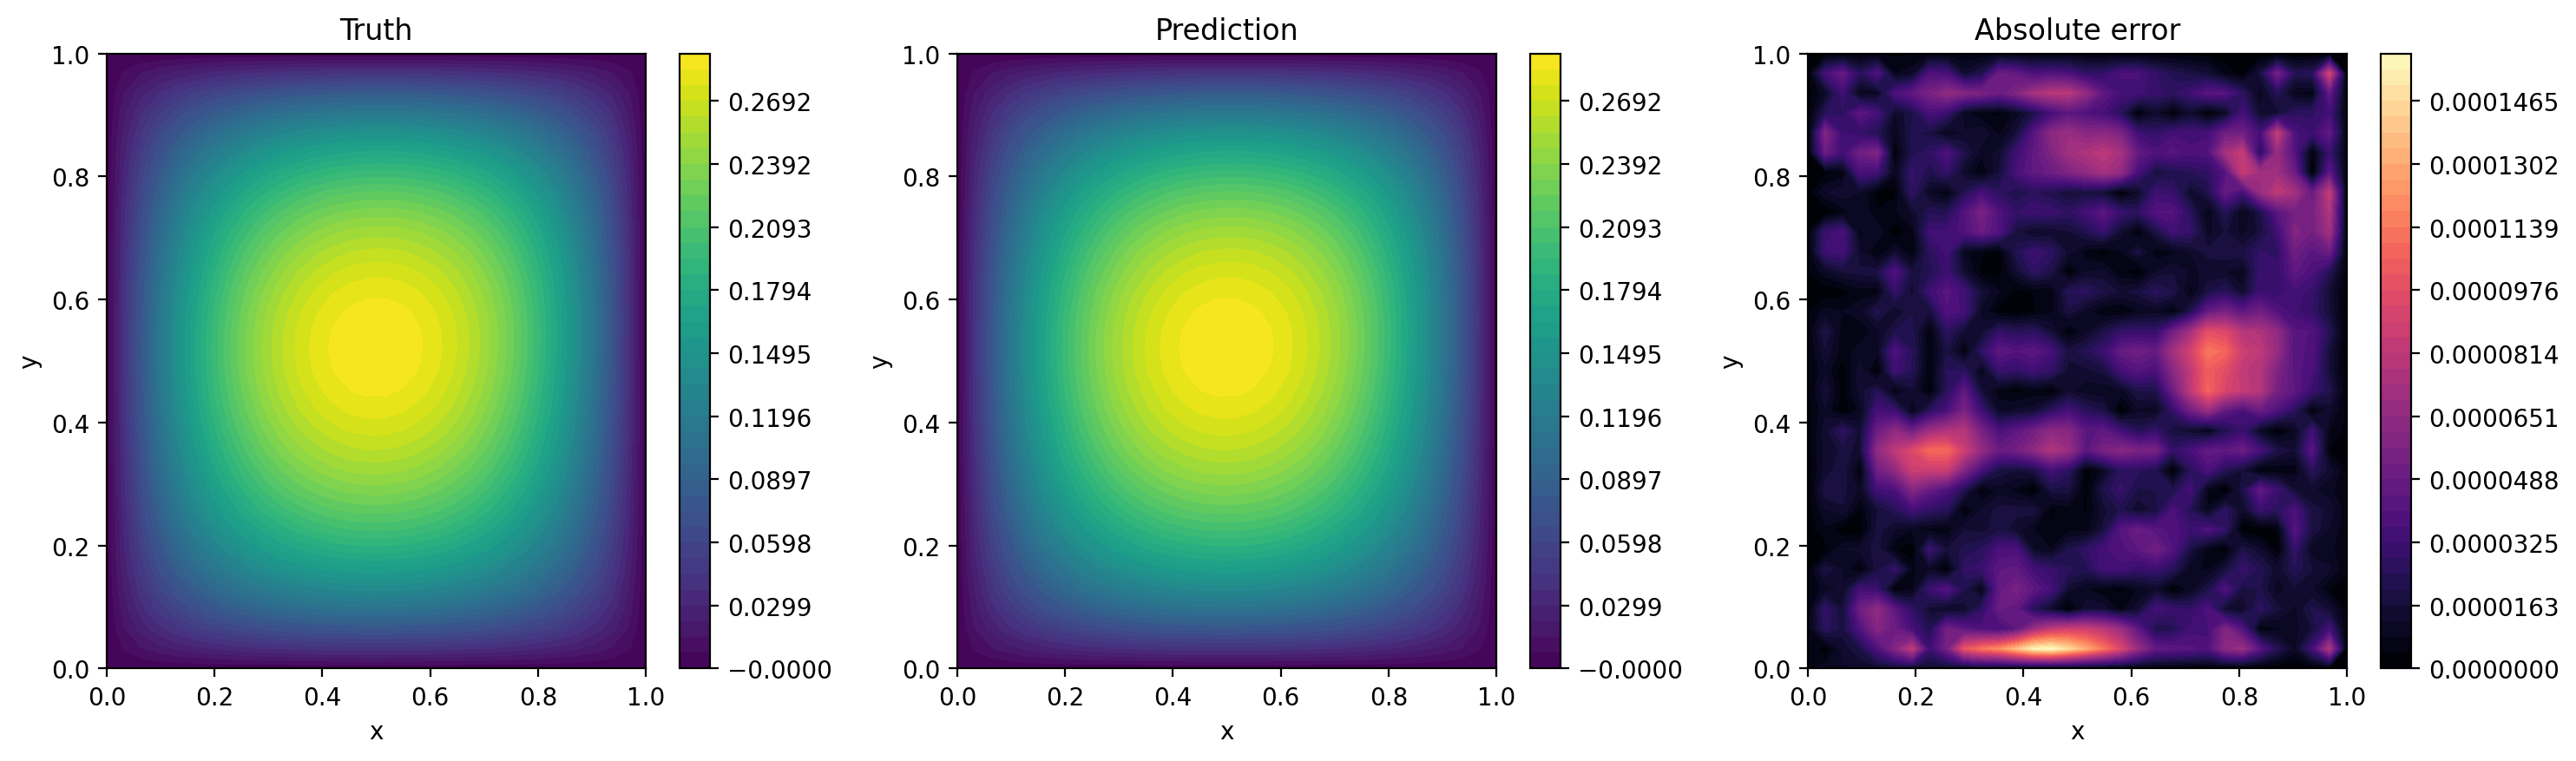
\includegraphics[width=\linewidth]{problem_2_outputs/darcy_fno/20260316_124531_single_final/figures/prediction_comparison.png}
    \caption{CPU FNO truth, prediction, and absolute error for a test sample. The prediction follows the target field extremely closely, and the error is much weaker than for either CNN-based model.}
\end{figure}

Once trained on CPU, the FNO was the strongest model. The error field is weaker and more uniform than for either the simple CNN or the U-Net, which is consistent with the FNO's ability to capture global structure efficiently in operator-learning problems.

\subsection*{Backend Sensitivity and Numerical Reliability of the FNO}

The FNO required a dedicated reliability check because its initial final run on MPS produced FFT-related warnings and far worse performance than expected. To test whether this reflected a weakness of the architecture or a backend issue, the same hyperparameters were rerun on CPU.

\begin{table}[H]
\centering
\begin{tabular}{lrr}
\toprule
FNO run & Device & Final test loss \\
\midrule
Comparison run & MPS & 0.039111 \\
Canonical final run & CPU & 0.000772 \\
\bottomrule
\end{tabular}
\caption{Direct comparison of the two final FNO runs.}
\end{table}

This difference is extremely large: the CPU run improved the test loss by about 98.0\% relative to the MPS run.

\begin{figure}[H]
    \centering
    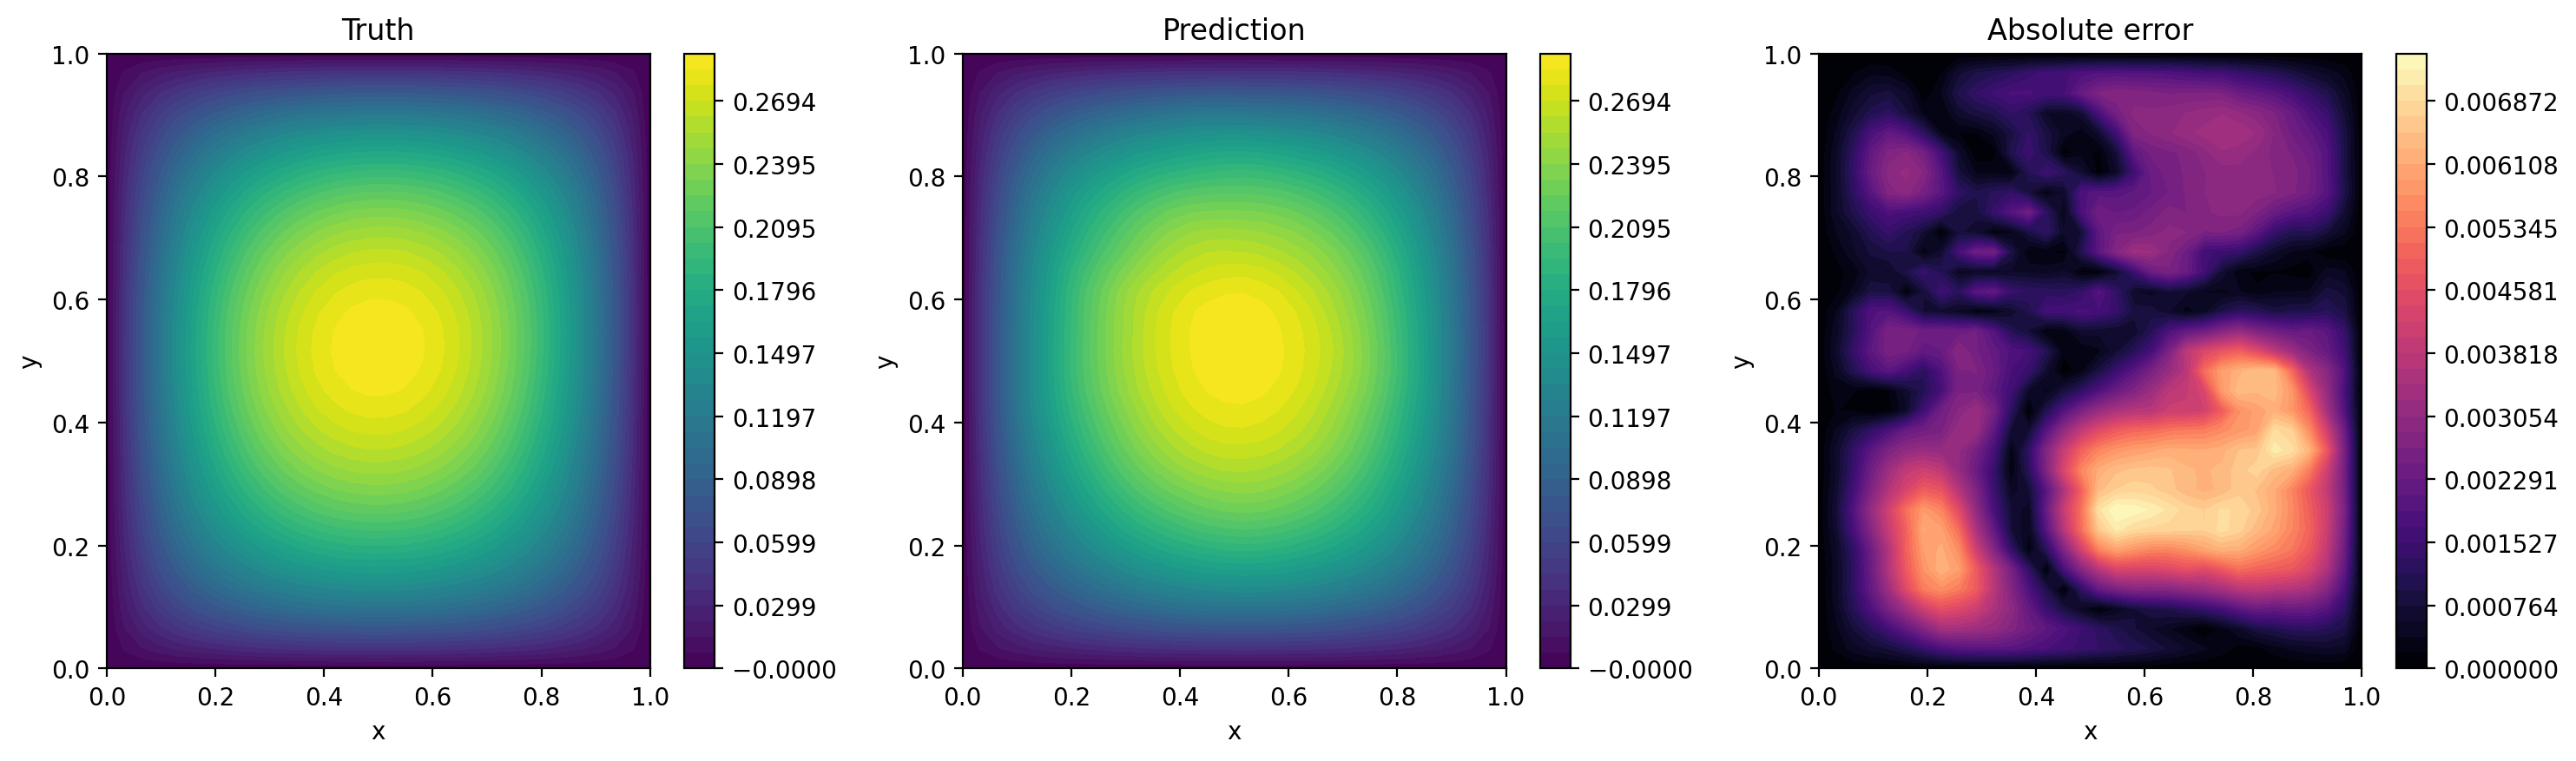
\includegraphics[width=\linewidth]{problem_2_outputs/darcy_fno/20260316_122017_single_final/figures/prediction_comparison.png}
    \caption{MPS FNO truth, prediction, and absolute error. The quality is much poorer than the CPU run despite identical architecture and hyperparameters, which strongly suggests a backend issue rather than an architectural failure.}
\end{figure}

This backend check materially changed the scientific interpretation of Problem 2. Without it, the FNO would have appeared to underperform the CNNs. With it, the FNO becomes the best model. The correct conclusion is therefore that the FNO architecture was strong, but the MPS FFT path was not reliable enough for this final configuration.

\subsection*{Problem 2 Discussion}

Once the backend issue was resolved, the model ordering became clear:
\begin{enumerate}[itemsep=0.25em]
    \item the simple CNN was already a strong baseline,
    \item the U-Net improved further by preserving multiscale detail through skip connections,
    \item the CPU FNO was best overall.
\end{enumerate}

This ordering is physically and numerically plausible. The simple CNN and U-Net are both very well suited to fixed-grid supervised PDE solution fields, while the FNO adds a spectral mechanism that can represent global structure more effectively. At the same time, the strength of the CNN baselines should not be underestimated: on a fixed \(32\times32\) grid, convolutional image-to-image models are already a natural fit.

\subsection*{Problem 2 Improvements}

If more time were available, the following improvements would be most valuable:
\begin{itemize}[itemsep=0.25em]
    \item broaden the hyperparameter search, especially for the FNO on CPU,
    \item tune epoch budgets more systematically,
    \item perform architecture ablations for the CNN and U-Net,
    \item report more than one qualitative test sample in the main text,
    \item compute additional summary metrics beyond relative \(L_2\),
    \item validate backend reliability earlier for FFT-heavy models.
\end{itemize}

These are discussed further in \path{problem_2_improvements.md}. The most important practical lesson is that backend checks should have been performed earlier for the FNO because they ultimately changed the interpretation of the entire architecture comparison.

\subsection*{Problem 2 Conclusion}

Problem 2 showed that convolutional models are already highly effective for the Darcy operator-learning task, with the U-Net improving on a strong simple CNN baseline. Once the backend issue was corrected, the FNO produced the best overall result by a wide margin. The final conclusion is therefore not that the FNO underperformed, but rather that it required a more reliable execution backend to demonstrate its full capability.

\section*{Short Overall Conclusion}

Across both coursework problems, the most important lesson was that internal optimization success is not the same as trustworthy scientific performance. In Problem 1, the physics-only PINN achieved an extremely low residual loss while still failing to match the FEM solution accurately. Adding only 50 displacement measurements transformed the result. In Problem 2, the model ranking changed substantially once the FNO was rerun on CPU rather than MPS.

The broader conclusion is that data-driven PDE methods must be judged using a combination of:
\begin{itemize}[itemsep=0.25em]
    \item physically meaningful validation metrics,
    \item careful graphical analysis,
    \item appropriate tuning strategies,
    \item and awareness of numerical issues such as precision and backend behaviour.
\end{itemize}

These factors were all essential to reaching defensible final conclusions in both coursework problems.

\appendix

\section{Additional Problem 1 Tuning Figures}

The following supplementary figures are available if a longer appendix is desired in the final PDF:
\begin{itemize}[itemsep=0.25em]
    \item \path{problem_1_experiments/optuna_studies/pinn_v4_baseline/figures/contour.png}
    \item \path{problem_1_experiments/optuna_studies/pinn_v4_baseline/figures/edf.png}
    \item \path{problem_1_experiments/optuna_studies/pinn_v4_baseline/figures/intermediate_values.png}
    \item \path{problem_1_experiments/optuna_studies/pinn_v4_baseline/figures/timeline.png}
    \item \path{problem_1_experiments/optuna_studies/pinn_v4_part_e/figures/contour.png}
    \item \path{problem_1_experiments/optuna_studies/pinn_v4_part_e/figures/edf.png}
    \item \path{problem_1_experiments/optuna_studies/pinn_v4_part_e/figures/intermediate_values.png}
    \item \path{problem_1_experiments/optuna_studies/pinn_v4_part_e/figures/timeline.png}
\end{itemize}

\section{Canonical Figure Sources}

\textbf{Problem 1}
\begin{itemize}[itemsep=0.25em]
    \item no-data PINN figures: \path{problem_1_figures/problem1_20260315_165315_full_nodata_seed1234/}
    \item data-assisted PINN figures: \path{problem_1_figures/problem1_20260315_203703_full_data_seed1234/}
\end{itemize}

\textbf{Problem 2}
\begin{itemize}[itemsep=0.25em]
    \item simple CNN final figures: \path{problem_2_outputs/darcy_cnn_simple/20260316_114818_single_final/figures/}
    \item U-Net final figures: \path{problem_2_outputs/darcy_cnn_unet/20260316_115014_single_final/figures/}
    \item FNO CPU final figures: \path{problem_2_outputs/darcy_fno/20260316_124531_single_final/figures/}
    \item FNO MPS comparison figures: \path{problem_2_outputs/darcy_fno/20260316_122017_single_final/figures/}
\end{itemize}

\end{document}
